% Preamble of the thesis. Structure on the model of the NHPSD MSc thesis of Gwade (2025);
% page design of our own: Charter body (XCharter), Fira Sans headings and figures, navy and
% teal accents, chapter openings with a large number, running header with the chapter.
% Citations: IEEE (school plan).
\documentclass[11pt,a4paper,oneside]{report}
% MiKTeX installs these fonts without registering their maps; loading the maps here keeps
% every font in Type 1 (otherwise pdfTeX falls back to bitmaps and microtype stops).
\pdfmapfile{+xcharter.map}
\pdfmapfile{+fira.map}
\pdfmapfile{+newtx.map}

% ---------------------------------------------------------------- fonts and language
\usepackage[T1]{fontenc}
\usepackage[utf8]{inputenc}
\usepackage[lining]{XCharter}
\usepackage[xcharter,vvarbb]{newtxmath}
\usepackage[scale=0.94,lining]{FiraSans}
\usepackage[scale=0.86]{FiraMono}
\usepackage[english]{babel}
\usepackage{microtype}

% ---------------------------------------------------------------- page
\usepackage[a4paper,top=2.6cm,bottom=2.6cm,left=2.6cm,right=2.6cm,headheight=14pt,headsep=0.9cm,footskip=1.1cm]{geometry}
\linespread{1.12}
\setlength{\parskip}{0.6em}
\setlength{\parindent}{0pt}
\usepackage[table]{xcolor}
\usepackage{tabularx,booktabs,longtable,multirow,array}
\usepackage{amsmath,mathtools,bm}
\usepackage{graphicx}
\usepackage{etoolbox}
\usepackage{tikz}
\usetikzlibrary{arrows.meta,positioning,shapes.geometric,fit,calc,backgrounds,decorations.pathreplacing}
\usepackage{pgfplots}
\pgfplotsset{compat=1.18}
\usepgfplotslibrary{groupplots}
\usepackage{subcaption}
\usepackage{float}
\usepackage{multicol}
\usepackage[most]{tcolorbox}

% ---------------------------------------------------------------- colours
\definecolor{cMain}{RGB}{24,52,89}       % navy: headings, rules
\definecolor{cAccent}{RGB}{0,122,135}    % teal: numbers, markers, links
\definecolor{cText2}{RGB}{90,96,104}     % secondary text: header, notes
\definecolor{cAfrica}{RGB}{192,57,43}    % figures: Douala, alerts
\definecolor{cRef}{RGB}{41,128,185}      % figures: development data
\definecolor{cGrey}{RGB}{127,140,141}    % figures: references
\arrayrulecolor{cMain!75}

% figures in the sans-serif face of the headings
\AtBeginEnvironment{tikzpicture}{\sffamily}
\pgfplotsset{every axis/.append style={tick label style={font=\scriptsize}, label style={font=\small},
  legend style={font=\footnotesize, draw=none}, axis line style={cText2}, tick style={cText2},
  scaled ticks=false, /pgf/number format/fixed}}

% ---------------------------------------------------------------- lists, captions, boxes
\usepackage{enumitem}
\setlist{topsep=0.25em,itemsep=0.2em}
\setlist[itemize]{label=\textcolor{cAccent}{\small$\blacktriangleright$}}
\setlist[enumerate]{label=\textcolor{cAccent}{\sffamily\bfseries\arabic*.}}
\setlist[description]{font=\sffamily\bfseries\color{cMain}}
\DeclareCaptionFont{navy}{\color{cMain}}
\usepackage[font=small,labelfont={sf,bf,navy},labelsep=quad,skip=6pt]{caption}
\newtcolorbox{keypoints}[1][Key points]{enhanced, colback=cMain!4, colframe=cMain!4,
  borderline west={2.5pt}{0pt}{cAccent}, sharp corners, left=10pt, right=10pt, top=7pt, bottom=7pt,
  fontupper=\small, before skip=12pt, after skip=12pt,
  title={#1}, coltitle=cMain, fonttitle=\sffamily\bfseries\small, attach title to upper={\par\smallskip}}

% floats: never before the paragraph that defines them; share pages with text; float
% pages start at the top
\usepackage{flafter}
\renewcommand{\topfraction}{0.88}
\renewcommand{\bottomfraction}{0.7}
\renewcommand{\textfraction}{0.08}
\renewcommand{\floatpagefraction}{0.8}
\setcounter{topnumber}{3}
\setcounter{bottomnumber}{2}
\setcounter{totalnumber}{5}
\makeatletter
\setlength{\@fptop}{0pt}
\makeatother

% ---------------------------------------------------------------- headings
\usepackage{needspace}
\usepackage{titlesec}
\setcounter{secnumdepth}{2}
\setcounter{tocdepth}{2}
\titleformat{\chapter}[display]
  {\normalfont\sffamily\color{cMain}}
  {{\small\bfseries\color{cAccent}\MakeUppercase{\chaptertitlename}}\hspace{0.5em}%
   {\fontsize{50}{50}\selectfont\bfseries\color{cMain!22}\thechapter}}
  {1.5ex}
  {\fontsize{23}{28}\selectfont\bfseries\raggedright}
  [{\vspace{1.6ex}\color{cAccent}\rule{3.2cm}{1.8pt}}]
\titleformat{name=\chapter,numberless}[display]
  {\normalfont\sffamily\color{cMain}}{}{0pt}
  {\fontsize{23}{28}\selectfont\bfseries\raggedright}
  [{\vspace{1.6ex}\color{cAccent}\rule{3.2cm}{1.8pt}}]
\titlespacing*{\chapter}{0pt}{0.6cm}{1.3cm}
\titleformat{\section}{\needspace{9\baselineskip}\normalfont\sffamily\bfseries\Large\color{cMain}}{\textcolor{cAccent}{\thesection}}{0.8em}{}
\titleformat{\subsection}{\needspace{5\baselineskip}\normalfont\sffamily\bfseries\large\color{cMain}}{\textcolor{cAccent}{\thesubsection}}{0.8em}{}
\titleformat{\subsubsection}{\normalfont\sffamily\bfseries\normalsize\color{cMain}}{}{0pt}{}
\titleformat{\paragraph}[runin]{\normalfont\sffamily\bfseries\color{cMain}}{}{0pt}{}[.]
\titlespacing*{\section}{0pt}{2.2ex plus 0.5ex}{0.8ex}
\titlespacing*{\subsection}{0pt}{1.7ex plus 0.4ex}{0.5ex}
\titlespacing*{\subsubsection}{0pt}{1.3ex plus 0.3ex}{0.3ex}
\titlespacing*{\paragraph}{0pt}{0.8ex}{0.6em}

% table of contents: chapters in the heading face
\usepackage{titletoc}
\titlecontents{chapter}[1.9em]{\addvspace{0.85em}\sffamily\bfseries\color{cMain}}
  {\contentslabel{1.9em}}{\hspace*{-1.9em}}{\hfill\contentspage}
\titlecontents{section}[4.4em]{\addvspace{0.15em}}
  {\contentslabel{2.5em}}{\hspace*{-2.5em}}{\titlerule*[0.7pc]{.}\contentspage}
\titlecontents{subsection}[7.5em]{\small}
  {\contentslabel{3.1em}}{\hspace*{-3.1em}}{\titlerule*[0.7pc]{.}\contentspage}

% ---------------------------------------------------------------- header and footer
\newcommand{\thesisauthor}{Nsame Ayuni Rodrick}
\newcommand{\shorttitle}{Telemonitoring of Hypertension and Diabetes}
\usepackage{fancyhdr}
\pagestyle{fancy}
\fancyhf{}
\renewcommand{\chaptermark}[1]{\markboth{\ifnum\value{chapter}>0 \thechapter\quad\fi #1}{}}
\renewcommand{\sectionmark}[1]{}
\fancyhead[L]{\sffamily\footnotesize\color{cText2}\leftmark}
\fancyhead[R]{\sffamily\footnotesize\bfseries\color{cMain}\thepage}
\renewcommand{\headrulewidth}{0.4pt}
\renewcommand{\headrule}{{\color{cMain!25}\hrule height\headrulewidth}}
\fancypagestyle{plain}{\fancyhf{}\fancyfoot[C]{\sffamily\footnotesize\color{cMain}\thepage}\renewcommand{\headrulewidth}{0pt}}
% unnumbered parts (Introduction, Conclusion) set their own header text
\newcommand{\unnumberedchapter}[1]{\chapter*{#1}\addcontentsline{toc}{chapter}{#1}\markboth{#1}{}}

% ---------------------------------------------------------------- bibliography (IEEE)
\usepackage[backend=biber,style=ieee,sorting=none,maxnames=3,minnames=1]{biblatex}
\addbibresource{references.bib}
\renewcommand*{\bibfont}{\small}

% ---------------------------------------------------------------- links (load last)
\usepackage[colorlinks=true,linkcolor=cMain,citecolor=cAccent,urlcolor=cAccent]{hyperref}
\usepackage[capitalise,noabbrev]{cleveref}
\hypersetup{pdftitle={Design of a Telemonitoring System for Patients with Hypertension and Diabetes},
  pdfauthor={Nsame Ayuni Rodrick}}


\begin{document}

% Front matter: title page, declaration, contents, acronyms, lists.
% Acknowledgments, Abstract and Résumé are added when the author sends the acknowledgments
% and the results are final.
\begin{titlepage}
% institutional band, bilingual as in Cameroonian university documents (logo space in the middle)
\begin{tikzpicture}[remember picture,overlay]
  \fill[cMain] (current page.north west) rectangle ([yshift=-4.4cm]current page.north east);
  \fill[cAccent] ([yshift=-4.4cm]current page.north west) rectangle ([yshift=-4.55cm]current page.north east);
  \node[anchor=north west, text=white, font=\sffamily\scriptsize, align=left, inner sep=0pt]
    at ([xshift=2.6cm,yshift=-1.0cm]current page.north west)
    {\textbf{REPUBLIC OF CAMEROON}\\ Peace -- Work -- Fatherland\\[4pt]
     \textbf{MINISTRY OF HIGHER EDUCATION}\\[4pt]
     \textbf{THE UNIVERSITY OF DOUALA}\\[4pt]
     \textbf{NATIONAL HIGHER POLYTECHNIC}\\ \textbf{SCHOOL OF DOUALA}};
  \node[anchor=north east, text=white, font=\sffamily\scriptsize, align=right, inner sep=0pt]
    at ([xshift=-2.6cm,yshift=-1.0cm]current page.north east)
    {\textbf{RÉPUBLIQUE DU CAMEROUN}\\ Paix -- Travail -- Patrie\\[4pt]
     \textbf{MINISTÈRE DE L'ENSEIGNEMENT SUPÉRIEUR}\\[4pt]
     \textbf{UNIVERSITÉ DE DOUALA}\\[4pt]
     \textbf{ÉCOLE NATIONALE SUPÉRIEURE}\\ \textbf{POLYTECHNIQUE DE DOUALA}};
\end{tikzpicture}
\raggedright\sffamily
\vspace*{3.6cm}

{\small\color{cText2} Laboratory of Computer Engineering, Data Science and Artificial Intelligence (LCEDSAI)}

\vspace{1.9cm}
{\small\bfseries\color{cAccent} MASTER'S THESIS}\\[0.45cm]
{\fontsize{26}{31}\selectfont\bfseries\color{cMain} Design of a Telemonitoring System\\ for Patients with Hypertension\\ and Diabetes}\\[0.5cm]
{\rmfamily\itshape\Large\color{cText2} Consultation data, home measurements and risk prediction}\\[0.5cm]
{\color{cAccent}\rule{3.2cm}{1.8pt}}

\vspace{1.5cm}
{\small\color{cText2} Presented by}\\[0.1cm]
{\Large\bfseries\color{cMain} Nsame Ayuni Rodrick}\\[0.55cm]
{\small\color{cText2} In partial fulfilment of the requirements for the degree of}\\[0.1cm]
{\large\bfseries Master of Science in Data Science and Artificial Intelligence}

\vspace{1.3cm}
\begin{tabular}{@{}l@{\hspace{2.2cm}}l@{}}
{\small\color{cText2} Supervisor} & {\small\color{cText2} Co-supervisor} \\[0.1cm]
{\large\bfseries Dr.\ Malong Yannick} & {\large\bfseries Dr.\ Noulapeu Ngaffo} \\
\end{tabular}

\vfill
{\color{cMain!30}\rule{\textwidth}{0.5pt}}\\[0.25cm]
{\small\color{cText2} Academic year 2025--2026 \hfill Douala, \today}
\end{titlepage}

\pagenumbering{roman}
\setcounter{page}{1}

\chapter*{Declaration}
\addcontentsline{toc}{chapter}{Declaration}
I, \textbf{Nsame Ayuni Rodrick}, declare that this Master's thesis entitled \emph{``Design of a Telemonitoring System for Patients with Hypertension and Diabetes''} is the result of my own research, carried out under the supervision of Dr.\ Malong Yannick and Dr.\ Noulapeu Ngaffo at the National Higher Polytechnic School of Douala (NHPSD), University of Douala, Cameroon.

I declare that, to the best of my knowledge, this work has not been submitted, in whole or in part, for any other degree, diploma or certification at any other institution.

I further declare that all sources of information, ideas and data used in this thesis have been acknowledged and referenced.

\vspace{3cm}
\hfill\begin{tabular}{l@{\hspace{0.3cm}}l}
Signed: & \rule{6cm}{0.4pt}\\[0.9cm]
Date: & \rule{6cm}{0.4pt}\\[0.9cm]
Place: & \rule{6cm}{0.4pt}
\end{tabular}

\cleardoublepage
\phantomsection\addcontentsline{toc}{chapter}{Contents}
\tableofcontents

\chapter*{List of Acronyms}\addcontentsline{toc}{chapter}{List of Acronyms}
{\small
\begin{multicols}{2}\raggedright
\textbf{ADA} American Diabetes Association\\
\textbf{AI} Artificial intelligence\\
\textbf{AUC} Area under the curve\\
\textbf{AUROC} Area under the ROC curve\\
\textbf{BP} Blood pressure\\
\textbf{CI} Confidence interval\\
\textbf{CPU, GPU} Central, graphics processing unit\\
\textbf{DBP} Diastolic blood pressure\\
\textbf{ECG} Electrocardiogram\\
\textbf{eICU} eICU Collaborative Research Database\\
\textbf{ENSPD} \'Ecole Nationale Sup\'erieure Polytechnique de Douala (NHPSD)\\
\textbf{ESH} European Society of Hypertension\\
\textbf{GRU-D} Gated recurrent unit with decay\\
\textbf{HbA1c} Glycated haemoglobin\\
\textbf{HEARTS} WHO technical package for cardiovascular care\\
\textbf{IHSG} International Hypoglycaemia Study Group\\
\textbf{IoT} Internet of Things\\
\textbf{LASSO} Least absolute shrinkage and selection operator\\
\textbf{LSTM} Long short-term memory\\
\textbf{MAD} Median absolute deviation\\
\textbf{MAR, MCAR, MNAR} Missing at random, completely at random, not at random\\
\textbf{mHealth} Mobile health\\
\textbf{MQTT} Message Queuing Telemetry Transport\\
\textbf{NEWS2} National Early Warning Score 2\\
\textbf{NHPSD} National Higher Polytechnic School of Douala\\
\textbf{PCA} Principal component analysis\\
\textbf{PPG} Photoplethysmography\\
\textbf{PRISMA} Preferred Reporting Items for Systematic Reviews and Meta-Analyses\\
\textbf{PROBAST} Prediction model Risk Of Bias Assessment Tool\\
\textbf{RCT} Randomised controlled trial\\
\textbf{ROC} Receiver operating characteristic\\
\textbf{RPS} Ranked probability score\\
\textbf{RQ} Research question\\
\textbf{SBP} Systolic blood pressure\\
\textbf{SD} Standard deviation\\
\textbf{SDK} Software development kit\\
\textbf{SHAP} Shapley additive explanations\\
\textbf{SMS} Short message service\\
\textbf{STEPS} WHO STEPwise approach to surveillance\\
\textbf{TPE} Tree-structured Parzen estimator\\
\textbf{TRIPOD} Transparent Reporting of a multivariable prediction model for Individual Prognosis Or Diagnosis\\
\textbf{WHO} World Health Organization
\end{multicols}}

\cleardoublepage\phantomsection
\addcontentsline{toc}{chapter}{List of Figures}
\listoffigures

\cleardoublepage\phantomsection
\addcontentsline{toc}{chapter}{List of Tables}
\listoftables

\clearpage
\pagenumbering{arabic}
\setcounter{page}{1}


%==========================================================================
% INTRODUCTION (unnumbered)
%==========================================================================
\unnumberedchapter{Introduction}\label{ch:intro}

Hypertension is the leading modifiable risk factor for premature death worldwide. The number of adults aged 30--79 years living with hypertension doubled between 1990 and 2019 to reach 1.3 billion, about 78\% of whom live in low- and middle-income countries, and elevated systolic blood pressure causes an estimated 10.8 million deaths each year \parencite{who2023hypertension}. Sub-Saharan Africa combines a high and rising prevalence with poor detection, treatment and control \parencite{gafane2024}: in the WHO African Region only 12\% of hypertensive adults have their blood pressure controlled. Diabetes compounds the burden. In Africa, 58\% of people living with diabetes are also hypertensive \parencite{hinneh2023}; the two conditions share their risk factors, aggravate each other, and call for the same care: repeated measurement and treatment adjusted over decades.

\section*{The Follow-up Challenge}

Care for hypertension and diabetes in Cameroon is episodic. Blood pressure and glucose are measured at consultations a few times a year, recorded on paper, and rarely assembled into a history that a clinician can read as a trend. Yet diagnosis and treatment adjustment are longitudinal acts: the WHO protocol requires measurements repeated over several visits and monthly follow-up until the target is reached \parencite{who2021guideline,who2023hypertension}. Two failures follow. Loss to follow-up affects half of patients or more in resource-limited settings, and therapeutic inertia leaves treatment unchanged while blood pressure stays above target \parencite{who2023hypertension}. In the African Region, 72\% of the patients already diagnosed are not controlled: they are known to the health system and lost during follow-up.

\section*{The Potential of Telemonitoring and Prediction}

Mobile telephony now reaches most of the population \parencite{segun2025}, and a controlled study in Cameroonian district hospitals has shown that remote clinical support is feasible in primary care \parencite{bediang2021}. Telemonitoring, the transmission of home measurements to a care team, lowers systolic pressure by 3 to 7~mmHg and glycated haemoglobin by 0.4 to 0.5 points, provided a clinician acts on the data \parencite{mao2020,mihevc2025}. Where clinicians are scarce, the system must also decide which readings deserve their time. The only validated protocol for patients with both conditions sorts readings into three levels with fixed thresholds \parencite{mihevc2025}: it reacts to the level of a reading, not to its trend, and uses no learned model. Machine learning could forecast deterioration from a patient's own series, but the reported results of the field are fragile. The same algorithm is reported as the best on one dataset \parencite{efendi2025} and as no better than chance on another \parencite{mendoza2025}, because the first study predicts a label already encoded in its inputs.

\section*{Research Problem and Motivation}

This thesis addresses two problems.
\begin{enumerate}
  \item \textbf{A practical problem.} No telemonitoring system evaluated in Central Africa combines consultation records, home measurements and a predictive model for patients with hypertension and diabetes, and orders the clinician's attention under intermittent connectivity and scarce specialist time \parencite{dodoo2022,agbeyangi2025}.
  \item \textbf{A methodological problem.} The predictive results of the field rest on labels that leak into the features, improper metrics and validation on the training population. Whether a learned model forecasts deterioration better than the guideline rule, and whether a model developed elsewhere transfers to Cameroonian patients, has not been measured.
\end{enumerate}

The data available to this work were not collected at home. The public eICU Collaborative Research Database, which records intensive-care stays in United States hospitals, is used to develop and compare the models. The observation charts of 32 patients hospitalised in Douala, with blood pressure, pulse and glucose recorded morning and evening, are used only to validate them externally. No home measurement or sensor data were collected: the system is built for home follow-up, but its predictive component is evaluated on hospital data, and its transfer to home data remains to be established.

\section*{Objectives and Research Questions}

The general objective is to design a telemonitoring system for patients with hypertension and type~2 diabetes that supports the clinician through risk assessment and alert prioritisation, and to evaluate its predictive component without the biases of previous work. The specific objectives are:
\begin{itemize}
  \item to derive the requirements of the system and the gaps of the field from the literature (\cref{ch:review});
  \item to formalise the risk-tiering problem: a sourced labelling rule, a forecasting task free of label leakage, and the combination of rule and model (\cref{ch:framework});
  \item to build a documented pipeline of data collection and treatment, and a benchmark protocol that selects the model instead of presupposing it (\cref{ch:methodology});
  \item to compare the candidate models on public multi-centre data, validate them externally on Cameroonian patients, and build the system around the result (\cref{ch:results}).
\end{itemize}

Four research questions follow:
\begin{description}
  \item[RQ1.] Can a telemonitoring system combining consultation records, home readings and risk prediction be built under the connectivity, workload and cost constraints of Cameroonian care?
  \item[RQ2.] Do learned models forecast the risk level of the next reading better than the guideline rule, and does a deep temporal model outperform classical models?
  \item[RQ3.] Does the advantage persist when the forecast is made 24 and 48 hours ahead?
  \item[RQ4.] Do models developed on another health system transfer to Cameroonian patients?
\end{description}

\section*{Hypotheses}

RQ1 is a design question, answered by the system and by the traceability of each of its elements to a requirement. RQ2 to RQ4 lead to four testable hypotheses, stated with the measures of \cref{sec:metrics}:
\begin{description}
  \item[H1.] At least one learned model forecasts the level of the next reading with a lower ranked probability score than the guideline rule applied to the last reading (persistence).
  \item[H2.] This advantage persists at lead times of 24 and 48~hours.
  \item[H3.] The deep temporal models do not outperform the tabular models.
  \item[H4.] Performance is lower on the Douala patients than on the development data, and updating the intercept on the local data recovers part of the calibration.
\end{description}

\section*{Contributions and Thesis Outline}

This work contributes:
\begin{itemize}
  \item \textbf{A data collection and treatment pipeline}: a labelling rule in which every threshold comes from an official source, quality controls that tell artefacts from events, an analysis of the instruments from the readings themselves, and the harmonisation of intensive-care records to the rhythm of ward charts.
  \item \textbf{A benchmark protocol}: candidates taken from published benchmarks rather than chosen in advance, nested validation grouped by hospital, proper scoring rules combined in a declared selection cost, and external validation on Cameroonian patients. The same discipline selects the measure that tracks the evolution of a patient's state.
  \item \textbf{A telemonitoring system}: a patient application and a clinician dashboard implementing the three-level home protocol, a local risk service sharing the code of the benchmark, and server functions for escalation, reminders and verdicts.
\end{itemize}

\begin{figure}[htbp]
\centering
\begin{tikzpicture}[font=\scriptsize, node distance=0.32cm,
  ch/.style={draw=cMain!60, rounded corners=2pt, align=center, text width=2.05cm, minimum height=2.3cm, fill=white, anchor=north},
  hd/.style={font=\scriptsize\bfseries, text=cMain},
  arr/.style={-{Stealth[length=1.8mm]}, semithick, cMain}]
  \node[ch, fill=cMain!6] (i) {{\color{cAccent}\bfseries Introduction}\\[3pt] problem, questions RQ1--RQ4, hypotheses};
  \node[ch, right=of i.north east, anchor=north west] (c1) {{\color{cAccent}\bfseries Chapter 1}\\[3pt] literature: what is known, the five gaps};
  \node[ch, right=of c1.north east, anchor=north west] (c2) {{\color{cAccent}\bfseries Chapter 2}\\[3pt] framework: label, forecast, decision layer};
  \node[ch, right=of c2.north east, anchor=north west] (c3) {{\color{cAccent}\bfseries Chapter 3}\\[3pt] data, treatment, benchmark protocol, system};
  \node[ch, right=of c3.north east, anchor=north west] (c4) {{\color{cAccent}\bfseries Chapter 4}\\[3pt] results: data, models, system; discussion};
  \node[ch, fill=cMain!6, right=of c4.north east, anchor=north west] (cc) {{\color{cAccent}\bfseries Conclusion}\\[3pt] findings and future work};
  \foreach \a/\b in {i/c1, c1/c2, c2/c3, c3/c4, c4/cc} \draw[arr] (\a.east) -- (\b.west);
  \draw[decorate, decoration={brace, amplitude=4pt, mirror}, cText2] ([yshift=-3pt]c3.south west) -- node[below=5pt, text=cText2]{RQ1: the system} ([yshift=-3pt]c4.south east);
  \draw[decorate, decoration={brace, amplitude=4pt, mirror}, cText2] ([yshift=-17pt]c2.south west) -- node[below=5pt, text=cText2]{RQ2--RQ4: the predictive component} ([yshift=-17pt]c4.south east);
\end{tikzpicture}
\caption{Organisation of the thesis and where each research question is answered.}\label{fig:roadmap}
\end{figure}

\Cref{fig:roadmap} summarises the organisation. \Cref{ch:review} reviews the clinical and technical literature and identifies the gaps. \Cref{ch:framework} formalises the risk-tiering problem. \Cref{ch:methodology} describes the data, their treatment, the benchmark protocol and the system. \Cref{ch:results} reports the results and discusses them, and the Conclusion summarises the findings and the directions for future work. Every number of the results is produced by a script of the accompanying code, which can be rerun.


%==========================================================================
% CHAPTER 1 -- THEORETICAL FOUNDATIONS AND LITERATURE REVIEW
%==========================================================================
\chapter{Theoretical Foundations and Literature Review}\label{ch:review}\label{ch:background}\label{ch:litreview}

This chapter establishes what is known about the burden of hypertension and diabetes and the failure of their care, the clinical evidence for telemonitoring, the instruments and architectures available, and the use of machine learning for clinical risk. It draws on nineteen peer-reviewed sources, each checked against PubMed, Crossref or the publisher's record, complemented by the guidelines of the World Health Organization (WHO) \parencite{who2023hypertension,who2021guideline,whoHEARTS} and of the European Society of Hypertension (ESH) \parencite{mancia2023}. Each study is reported with its method, its main result and its limits, in six themes (\cref{tab:lr-overview}); the chapter ends with a comparison of the approaches and the gaps that motivate this work.

\begin{table}[htbp]
\centering\footnotesize
\caption{Sources of the review, by theme and in chronological order within each theme.}\label{tab:lr-overview}
\begin{tabularx}{\textwidth}{@{}>{\raggedright\arraybackslash}p{3.4cm} >{\raggedright\arraybackslash}p{3.9cm} >{\raggedright\arraybackslash}X@{}}
\toprule
\textbf{Theme} & \textbf{Source} & \textbf{Design and setting} \\
\midrule
1. Burden of disease & \textcite{hinneh2023} & systematic review and meta-analysis, Africa \\
 & \textcite{who2023hypertension} & institutional global report \\
\addlinespace
2. Care and digital health in sub-Saharan Africa & \textcite{kingue2013} & interventional pilot, rural Cameroon \\
 & \textcite{bediang2021} & controlled multicentre study, Cameroon \\
 & \textcite{dodoo2022} & review of 66 empirical studies, sub-Saharan Africa \\
 & \textcite{gafane2024} & narrative review, sub-Saharan Africa \\
 & \textcite{agbeyangi2025} & systematic review, South Africa, Kenya, Nigeria \\
 & \textcite{segun2025} & perspective, sub-Saharan Africa \\
\addlinespace
3. Mobile health and clinical evidence & \textcite{alessa2019} & review and content analysis of applications, United Kingdom \\
 & \textcite{mao2020} & meta-analysis of 51 randomised trials \\
 & \textcite{zhou2024} & meta-analysis of randomised trials \\
 & \textcite{bandeira2024} & updated meta-analysis of randomised trials \\
 & \textcite{mihevc2025} & multicentre randomised trial, Slovenia \\
\addlinespace
4. Sensors and IoT & \textcite{alhaddad2022} & review of non-invasive glucose sensing \\
 & \textcite{tai2024} & IoT architecture and deep learning technique \\
 & \textcite{efendi2025} & IoT and cloud implementation with device validation \\
 & \textcite{liu2025review} & review of IoT sensing and machine learning \\
 & \textcite{liu2025ppg} & smartphone photoplethysmography study \\
\addlinespace
5. Machine learning & \textcite{chatrati2022} & home monitoring system with machine learning \\
 & \textcite{mendoza2025} & cross-sectional predictive study, Mexico \\
\addlinespace
6. Privacy and ethics & \textcite{alhammad2024} & systematic review of patient perspectives \\
\bottomrule
\end{tabularx}
\end{table}

%--------------------------------------------------------------------------
\section{Key Concepts and Conceptual Framework}\label{sec:concepts}

The terms of \cref{tab:concepts} are used throughout the thesis with the meaning given here; several are used differently in the literature.

\begin{table}[htbp]
\centering\footnotesize
\caption{Key concepts and the definitions adopted in this thesis.}\label{tab:concepts}
\begin{tabularx}{\textwidth}{@{}>{\raggedright\arraybackslash}p{3.3cm} X@{}}
\toprule
\textbf{Concept} & \textbf{Definition adopted} \\
\midrule
Hypertension & systolic pressure $\geq 140$~mmHg, diastolic pressure $\geq 90$~mmHg, or antihypertensive treatment \parencite{who2023hypertension}; ESH grades from 140/90, 160/100 and 180/110~mmHg \parencite{mancia2023}; home threshold 135/85~mmHg \\
Type~2 diabetes & chronic hyperglycaemia due to insulin resistance and relative insulin deficiency; its follow-up requires a biological measurement (capillary or venous glucose, glycated haemoglobin) \\
Care cascade & nested stages of care---hypertensive, diagnosed, treated, controlled---measured on the same population \parencite{who2023hypertension} \\
Loss to follow-up & interruption of the planned follow-up of a patient already in care \\
Therapeutic inertia & failure to intensify treatment while blood pressure remains above target \\
Telemonitoring & transmission of physiological data from the patient's home to a care team, which provides clinical feedback \\
Mobile health (mHealth) & health practices supported by mobile devices: applications, text messages, connected devices \\
Self-measurement & measurement of blood pressure or capillary glucose by the patient at home, with a validated device and a standard protocol \\
Internet of Things (IoT) & connected devices that acquire and transmit data without human intervention \\
Clinical decision support & system that turns patient data into alerts or recommendations for a clinician, who keeps the decision \\
Supervised learning & estimation of a function mapping input features to a known label; here, a forecast of a future clinical state from a past window of readings \\
Label leakage & situation in which the label can be recovered from the inputs, so that measured performance reflects a rule rather than a prediction \\
Triage & ordering of readings or patients by priority for clinical review \\
\bottomrule
\end{tabularx}
\end{table}

Four models structure the reasoning (\cref{fig:concept-framework}). The \textbf{care cascade} locates where an intervention acts: screening acts on diagnosis, follow-up on treatment and control, where most diagnosed patients in Africa are lost. The \textbf{measurement model} treats a reading as the usual pressure plus an error that repeated readings reduce, which justifies series over isolated values. The \textbf{layered architecture} describes a monitoring system as a chain from acquisition to processing and presentation \parencite{tai2024,mucchi2021}. And \textbf{supervised learning for clinical prediction} fixes what a valid evaluation requires: a label outside the input window, proper measures, and a comparison with the guideline rule.

\begin{figure}[htbp]
\centering
\begin{tikzpicture}[node distance=0.35cm,
  b/.style={draw,rounded corners,align=center,font=\scriptsize,minimum height=1.1cm,text width=2.25cm},
  ar/.style={-{Stealth[length=2mm]},thick}]
  \node[b,fill=cAfrica!14] (p) {\textbf{Problem}\\ care cascade fails at follow-up};
  \node[b,fill=cGrey!14,right=of p] (m) {\textbf{Measurement}\\ repeated home readings};
  \node[b,fill=cRef!12,right=of m] (a) {\textbf{Record}\\ application, database, server functions};
  \node[b,fill=cRef!20,right=of a] (l) {\textbf{Prediction}\\ risk forecast from the series};
  \node[b,fill=cGrey!8,right=of l] (d) {\textbf{Decision}\\ triage and clinician review};
  \draw[ar] (p) -- (m); \draw[ar] (m) -- (a); \draw[ar] (a) -- (l); \draw[ar] (l) -- (d);
  \draw[ar,dashed,cAfrica] (d.south) -- ++(0,-0.45) -| node[near start,below,font=\tiny]{retention and treatment adjustment act back on the cascade} (p.south);
\end{tikzpicture}
\caption{Conceptual framework of the thesis.}\label{fig:concept-framework}
\end{figure}

%--------------------------------------------------------------------------
\section{Burden of Hypertension and Diabetes}\label{sec:burden}\label{sec:hta-burden}

\subsection{The care cascade}\label{sec:cascade}

For population surveillance, the WHO defines hypertension as a systolic blood pressure (SBP) $\geq 140$~mmHg, a diastolic blood pressure (DBP) $\geq 90$~mmHg, or the use of antihypertensive medication \parencite{who2023hypertension}; the ESH uses the same threshold and divides hypertension into three grades \parencite{mancia2023}. The number of hypertensive adults rose from 650 million in 1990 to 1.3 billion in 2019, while the age-standardised prevalence barely changed, from 32\% to 33\%: population growth and ageing, not individual risk, drive the increase. Elevated systolic pressure is the leading risk factor for premature death among the 87 compared.

The WHO describes care as a cascade of nested stages measured on the same denominator (\cref{tab:cascade}). The European Region has a higher prevalence than the African Region but a control rate more than twice as high: the African deficit is organisational rather than epidemiological. In the African Region, 57\% of hypertensive adults are undiagnosed, 37\% of the diagnosed are untreated and 56\% of the treated are not controlled; among patients already diagnosed, 72\% are not controlled. Screening acts on the first link of the chain; longitudinal follow-up acts on the second and third.

\begin{table}[htbp]
\centering\small
\caption{Hypertension care cascade by WHO region, adults aged 30--79 years, 2019 \parencite{who2023hypertension}.}\label{tab:cascade}
\begin{tabular}{@{}lcccc@{}}
\toprule
\textbf{Indicator} & \textbf{African Region} & \textbf{World} & \textbf{Americas} & \textbf{Europe} \\
\midrule
Age-standardised prevalence & 36\% & 33\% & 35\% & 37\% \\
Diagnosis coverage & 43\% & 54\% & 70\% & 66\% \\
Treatment coverage & 27\% & 42\% & 60\% & 53\% \\
Effective treatment (control) & 12\% & 21\% & 36\% & 26\% \\
\bottomrule
\end{tabular}
\end{table}

\subsection{The hypertension--diabetes comorbidity}\label{sec:comorbidity}

Diabetes stiffens small vessels, which raises peripheral resistance and blood pressure, and hypertension accelerates the vascular damage of diabetes. \Textcite{hinneh2023} pooled 41 cross-sectional studies (144\,433 participants) following PRISMA: 58.1\% of people with diabetes in Africa are also hypertensive (95\% CI 52.0--63.2), and 60.8\% of those with type~2 diabetes. The risk rises with age, excess weight, years lived with diabetes, urban residence and male sex. The sub-regional estimates place Central Africa highest (\cref{tab:subregional,fig:forest}).

\begin{table}[htbp]
\centering\small
\caption{Sub-regional pooled prevalence of hypertension among people with diabetes in Africa \parencite{hinneh2023}.}\label{tab:subregional}
\begin{tabular}{@{}lccc@{}}
\toprule
\textbf{Sub-region} & \textbf{Pooled prevalence} & \textbf{95\% CI} & \textbf{Studies} \\
\midrule
Central Africa & 77.6\% & 53.0--91.4 & 2 \\
Southern Africa & 69.1\% & 59.8--77.1 & 10 \\
Eastern Africa & 53.0\% & 45.8--59.1 & 15 \\
Western Africa & 51.5\% & 41.8--61.1 & 10 \\
\bottomrule
\end{tabular}
\end{table}

\begin{figure}[htbp]
\centering
\begin{tikzpicture}
\begin{axis}[width=0.82\textwidth,height=5.2cm,xlabel={Pooled prevalence of hypertension among people with diabetes (\%)},
  xmin=30,xmax=100,ymin=0.5,ymax=5.5,ytick={1,2,3,4,5},
  yticklabels={Western Africa,Eastern Africa,Southern Africa,Central Africa,All Africa},
  grid=major,grid style={gray!20}]
\addplot[dashed,cGrey,no markers] coordinates {(58.1,0.5)(58.1,5.5)};
\addplot[only marks,mark=*,mark size=2.5pt,cRef,error bars/.cd,x dir=both,x explicit,error bar style={thick}]
  coordinates {(51.5,1) += (9.6,0) -= (9.7,0)
               (53.0,2) += (6.1,0) -= (7.2,0)
               (69.1,3) += (8.0,0) -= (9.3,0)};
\addplot[only marks,mark=*,mark size=2.5pt,cAfrica,error bars/.cd,x dir=both,x explicit,error bar style={thick}]
  coordinates {(77.6,4) += (13.8,0) -= (24.6,0)};
\addplot[only marks,mark=square*,mark size=2.5pt,black,error bars/.cd,x dir=both,x explicit,error bar style={thick}]
  coordinates {(58.1,5) += (5.1,0) -= (6.1,0)};
\end{axis}
\end{tikzpicture}
\caption{Estimates and 95\% intervals of \cref{tab:subregional}; the dashed line marks the pooled African estimate. The Central African interval spans 38 points.}\label{fig:forest}
\end{figure}

The Central African value must be read with its interval. It rests on two small Cameroonian hospital series (109 and 210 patients), while three other Central African studies listed in the article (1\,832 patients, prevalences of 35.0--50.4\%) do not enter the subgroup; heterogeneity is extreme ($I^2 \approx 98\%$), and the restriction to English-language publications under-represents francophone Central Africa. It cannot carry the case for this work on its own. That case rests on the continental estimate, on the mechanism, and on the WHO position that uncontrolled hypertension is among the risk factors most strongly associated with premature death in people with diabetes \parencite{who2023hypertension}. More generally, the prevalences quoted in this chapter differ in population, threshold, number of measurement visits and recruitment; none is nationally representative for Cameroon, so the nature of each estimate is stated where it is used.

\subsection{Why one reading is not enough}\label{sec:variability}\label{sec:dx-requires}\label{sec:followup-requires}

The WHO diagnostic protocol is longitudinal by construction: hypertension is diagnosed only if the threshold is exceeded at two visits \parencite{who2023hypertension}. A reading of patient $i$ at time $t$ can be written $b_{i,t} = \mu_i + \varepsilon_{i,t}$, where $\mu_i$ is the patient's usual pressure, the clinically relevant quantity, and $\varepsilon_{i,t}$ gathers circadian variation, activity, the measurement setting and instrument error. With $n$ readings far enough apart for their errors to be independent,
\begin{equation}
  \operatorname{Var}(\hat\mu_i) = \sigma_\varepsilon^2 / n .
\end{equation}
A consultation provides two to four readings a year; home follow-up provides several dozen, which estimate $\mu_i$ far more precisely and also estimate the patient's own variability $\sigma_\varepsilon$. Follow-up must moreover be frequent: Recommendation~7 of the WHO guideline sets monthly follow-up after a treatment change until the target is reached, then every three to six months \parencite{who2021guideline}. With 56\% of treated patients uncontrolled, this means about eight contacts per patient per year, where an episodic model delivers one or two.

%--------------------------------------------------------------------------
\section{Hypertension Care and Digital Health in Sub-Saharan Africa}\label{sec:lr-regional}\label{sec:diagnosis}

\subsection{Why the episodic model fails}\label{sec:ltfu}\label{sec:inertia}

\Textcite{gafane2024} synthesise the hypertension literature of sub-Saharan Africa from 2017 to 2023: a high burden with poor detection and control, driven by a westernised lifestyle, and obstacles to care that are individual (literacy, cost, distance) and systemic (medicines, staffing). Their inventory of national surveys is the most recent for Central Africa (\cref{tab:central-africa}): prevalence ranges from 13.5\% to 42.1\%, reflecting the diversity of instruments as much as real differences, and three countries have no data. In Cameroon, the May Measurement Month campaign of 2019 found a prevalence of 20.8\%, with only 11.2\% of hypertensive participants controlled.

\begin{table}[htbp]
\centering\footnotesize
\caption{Most recent hypertension surveys in Central Africa (adapted from \cite{gafane2024}, Table~1).}\label{tab:central-africa}
\begin{tabularx}{\textwidth}{@{}l >{\raggedright\arraybackslash}X c r r r r r@{}}
\toprule
\textbf{Country} & \textbf{Instrument} & \textbf{Year} & \textbf{$n$} & \textbf{Prev.} & \textbf{Aware.} & \textbf{Treat.} & \textbf{Control} \\
\midrule
Burundi & hospital screening & 2018 & 353 & 16.7\% & -- & -- & -- \\
Cameroon & May Measurement Month & 2019 & 30\,167 & 20.8\% & 29.9\% & 24.0\% & 11.2\% \\
Central African Rep. & WHO STEPS & 2017 & 3\,265 & 42.1\% & 30.2\% & -- & -- \\
Comoros & national survey & 2019 & 2\,602 & 38.4\% & 47.9\% & 45.4\% & 30.2\% \\
DR Congo & May Measurement Month & 2019 & 29\,857 & 25.5\% & 33.1\% & 23.2\% & 11.9\% \\
Congo (Rep.) & May Measurement Month & 2019 & 3\,157 & 33.5\% & 42.6\% & 37.3\% & 23.3\% \\
Gabon & retrospective study & 2013--15 & 2\,104 & 13.5\% & -- & -- & -- \\
Chad, Eq.\ Guinea, S\~ao Tom\'e & no data & -- & -- & -- & -- & -- & -- \\
\bottomrule
\end{tabularx}
\end{table}

The WHO documents the mechanisms \parencite{who2023hypertension}: loss to follow-up often affects half of patients or more, so screening is useful only when linked to follow-up; therapeutic inertia makes the last link the weakest; lifestyle change alone lowers systolic pressure by only about 1.3~mmHg, so nearly every patient needs medication and its timely adjustment; consultations often last less than five minutes; and paper records are lost or unavailable during the visit.

\subsection{Telemedicine evidence from Cameroon}\label{sec:telemedcam}\label{sec:bediang}\label{sec:cameroon-joint}

Two controlled evaluations of cardiovascular telemedicine have been conducted in Cameroonian primary care (\cref{tab:cameroon-pair}). In TELEMED-CAM, \textcite{kingue2013} supported thirty rural health centres from Yaoundé: among 268 participants followed for 24 weeks, attendance at scheduled visits was higher in the intervention arm at every grade of hypertension, but the benefit on control was confined to stage~III. \Textcite{bediang2021} equipped two district hospitals with an electrocardiograph and a tele-expertise platform: access to an electrocardiogram with a cardiologist's opinion reached 98.9\% against 33.3\%, and the expert modified the local diagnosis in 46.2\% of cases. The specialist's opinion, however, took 10.3 days on average against a protocol maximum of 72 hours, no faster than in the control centres: the bottleneck was expert availability, not transmission.

\begin{table}[htbp]
\centering\footnotesize
\caption{The two Cameroonian evaluations of cardiovascular telemedicine.}\label{tab:cameroon-pair}
\begin{tabularx}{\textwidth}{@{}>{\raggedright\arraybackslash}p{2.5cm} >{\raggedright\arraybackslash}X >{\raggedright\arraybackslash}X@{}}
\toprule
 & \textbf{\textcite{kingue2013}} & \textbf{\textcite{bediang2021}} \\
\midrule
Function & telemanagement of treatment & tele-expertise for diagnosis \\
Design & partly randomised by centre, 268 patients & matched centres, not randomised, 171 patients \\
Principal result & control improved in stage~III only & ECG with expertise, 98.9\% vs 33.3\% \\
Retention & visit adherence higher at every grade & 52 control patients not seen at 3 months \\
Main weakness & clustering ignored; effect of a package & non-comparable groups; differential attrition \\
\bottomrule
\end{tabularx}
\end{table}

Read together, the two studies support three conclusions. Retention is the most robust result, observed by different mechanisms eight years apart; an effect on blood pressure control is not established in Cameroon; and the value added lies in the clinical decision rather than in a tool placed in the patient's hands. Both show that systematic expert review of every case does not scale where specialists are scarce.

\subsection{Digital health landscape and barriers}\label{sec:digital-barriers}\label{sec:regional-landscape}

\Textcite{dodoo2022} reviewed 66 empirical studies of telemedicine in sub-Saharan Africa and grouped the barriers into six dimensions (\cref{tab:barriers}).

\begin{table}[htbp]
\centering\small
\caption{Six dimensions of barriers to telemedicine in sub-Saharan Africa \parencite{dodoo2022}.}\label{tab:barriers}
\begin{tabularx}{\textwidth}{@{}>{\raggedright\arraybackslash}p{3.4cm} X@{}}
\toprule
\textbf{Dimension} & \textbf{Definition given by the authors} \\
\midrule
Technological & information systems and connectivity \\
Organisational & stakeholder engagement, sustainability of systems \\
Individual & users' experience, knowledge and awareness \\
Financial & financial resources and operating cost \\
Cultural & social constraints and traditional beliefs \\
Legal and regulatory & policies, legislation, confidentiality and privacy protection \\
\bottomrule
\end{tabularx}
\end{table}

Most projects lost momentum once external funding ended, and health professionals facing a heavy workload perceived telemedicine as an additional task. \Textcite{agbeyangi2025} compared adoption in South Africa, Kenya and Nigeria over 53 studies; Central Africa is absent from the comparison. \Textcite{segun2025} report that more than 80\% of the population holds a mobile subscription, while about 550 million people lack reliable electricity and internet access and up to 18\% of countries had no registered cardiologist in 2020; artificial intelligence remains largely unvalidated on African populations. The population is reachable by mobile networks and the specialist is not: a system that forwards every reading reproduces the scarcity it should relieve, whereas one that sorts readings and orders the clinician's attention addresses it.

%--------------------------------------------------------------------------
\section{Mobile Health and Clinical Evidence}\label{sec:outpatient}\label{sec:evidence}

\Textcite{alessa2019} analysed the 186 hypertension applications of the two main stores in 2018: most offered a single function, none of the thirty analysed in depth had been evaluated scientifically, and they contained a median of nine behaviour change techniques. \Textcite{mao2020} pooled 51 randomised trials (13\,054 participants with diabetes or hypertension): mobile health lowered systolic pressure by 2.99~mmHg and glycated haemoglobin (HbA1c) by 0.39 points. Combined with professional management, it lowered systolic pressure by 6.17~mmHg; alone, by a non-significant 2.16~mmHg; and in developing countries, whose trials used no professional management, it had no effect on systolic pressure. Only one of the 51 trials took place in sub-Saharan Africa. \Textcite{zhou2024} found $-5.78$~mmHg over 16 trials of mobile applications, larger with at least eleven behaviour change techniques, and \textcite{bandeira2024} identify telemonitoring with clinician feedback as the most effective modality.

\subsection{A randomised trial in the target population}\label{sec:mihevc}

\Textcite{mihevc2025} ran the trial most relevant to this work: 128 patients aged 65 or more with both hypertension and type~2 diabetes, in three Slovenian primary-care centres. The intervention group measured blood pressure and glucose at home with Bluetooth devices transmitting to a cloud platform, and a telemedicine centre reviewed the values according to a three-level protocol (green, yellow, red) adopted in this work (\cref{sec:triage}). After twelve months, systolic pressure was 6.9~mmHg lower than in the control group and HbA1c 0.5 points lower. The authors credit the effect to contact with the care team and treatment adapted on reliable measurements, not to behaviour change. Seven of the 64 intervention patients (10.9\%) withdrew in the first month because they could not use the equipment, and a third of the systolic effect was lost between six and twelve months.

The clinical evidence (\cref{tab:effect-synthesis}) therefore supports a modest but clinically relevant effect, conditional on professional oversight. The evidence from sub-Saharan Africa is almost absent, and the absence of effect in developing countries is plausibly a design gap---no clinician at the end of the chain---rather than a context effect. Telemonitoring must be built as decision support linked to a clinician, not as a self-tracking tool.

\begin{table}[htbp]
\centering\footnotesize
\caption{Estimates of the effect of mobile health and telemonitoring on systolic pressure and glycaemic control.}\label{tab:effect-synthesis}
\begin{tabularx}{\textwidth}{@{}>{\raggedright\arraybackslash}p{4.3cm} >{\raggedright\arraybackslash}p{2.6cm} X >{\raggedright\arraybackslash}p{1.9cm}@{}}
\toprule
\textbf{Source} & \textbf{Design} & \textbf{Effect on SBP (95\% CI)} & \textbf{HbA1c} \\
\midrule
\textcite{mao2020}, overall & 30 RCTs on SBP & $-2.99$~mmHg ($-4.19$ to $-1.80$) & $-0.39$ \\
\quad with professional management & subgroup & $-6.17$~mmHg ($-8.83$ to $-3.50$) & -- \\
\quad developing countries & subgroup & $+0.25$~mmHg ($-3.10$ to $3.59$), n.s. & $-0.52$ \\
\textcite{zhou2024} & 16 RCTs & $-5.78$~mmHg ($-7.97$ to $-3.59$) & -- \\
\textcite{mihevc2025} & RCT, 128 patients & $-6.9$~mmHg ($-11$ to $-2.7$) & $-0.5$ \\
\bottomrule
\end{tabularx}
\end{table}

\begin{figure}[htbp]
\centering
\begin{tikzpicture}
\begin{axis}[width=0.84\textwidth, height=5.6cm,
  xlabel={effect on systolic blood pressure (mmHg)},
  xmin=-13, xmax=5, ymin=0.4, ymax=5.6, ytick={1,2,3,4,5},
  yticklabels={Mao 2020{,} developing countries, Mao 2020{,} with professional, Mao 2020{,} overall, Zhou 2024, Mihevc 2025},
  y tick label style={font=\scriptsize}, xmajorgrids, grid style={cGrey!20}]
\addplot[dashed, cText2, no markers] coordinates {(0,0.4) (0,5.6)};
\addplot[only marks, mark=square*, mark size=2.4pt, cRef, error bars/.cd, x dir=both, x explicit, error bar style={thick}]
  coordinates {(-6.90,5) += (4.20,0) -= (4.10,0)
               (-5.78,4) += (2.19,0) -= (2.19,0)
               (-2.99,3) += (1.19,0) -= (1.20,0)
               (-6.17,2) += (2.67,0) -= (2.66,0)};
\addplot[only marks, mark=*, mark size=2.4pt, cAfrica, error bars/.cd, x dir=both, x explicit, error bar style={thick}]
  coordinates {(0.25,1) += (3.34,0) -= (3.35,0)};
\end{axis}
\end{tikzpicture}
\caption{Estimates of \cref{tab:effect-synthesis} with their 95\% intervals. The only interval that includes no effect is that of the trials conducted in developing countries, none of which involved professional management.}\label{fig:sbp-forest}
\end{figure}

%--------------------------------------------------------------------------
\section{Devices, Sensors and Architectures}\label{sec:lr-iot}

\subsection{The normative position on devices}\label{sec:metrology}

The WHO recommends independently validated automated upper-arm cuffs and does not recommend cuffless devices for managing hypertension, because their accuracy and their ability to track change are unresolved; only about one automated device in five on the market has evidence of validation \parencite{who2023hypertension}. Non-invasive glucose sensing by electrocardiography, bioimpedance or photoplethysmography (PPG) shows promise for trends and hypoglycaemia but not for clinical-grade measurement \parencite{alhaddad2022}, and blood pressure from a smartphone camera correlates with reference devices on 127 participants but remains below cuff accuracy \parencite{liu2025ppg}. Blood pressure must therefore come from a validated cuff and glucose from a glucometer; PPG is at most a source of heart rate.

\subsection{IoT architectures for remote monitoring}

\Textcite{tai2024} embed a deep learning technique for chronic disease monitoring in a three-phase architecture---acquisition, processing, visualisation---evaluated in controlled conditions. \Textcite{efendi2025} built an Internet of Things (IoT) system for elderly people: an ESP32 microcontroller reads an optical heart-rate and oxygen sensor and a temperature sensor, sends the values over MQTT to a Firebase database with offline persistence, and displays them in a mobile application. Against a digital oximeter and thermometer, six volunteers measured for ten minutes gave a mean absolute percentage error of 0.90\%. The system measures neither blood pressure nor glucose. \Textcite{mucchi2021} decompose remote monitoring into body, environment, edge and cloud layers and tested their system with ten nurses on simulated patients; \textcite{yazdani2018} add a priority-ordered clinician queue and a configurable checkup period, without implementing them; \textcite{liu2025review} survey IoT sensing with machine learning and describe the defects of electronic records: duplicates, unit errors and values carried over. The architectures converge on acquisition, transmission and storage, processing and presentation; none has been validated on patients in routine care in a low-resource setting.

%--------------------------------------------------------------------------
\section{Machine Learning for Clinical Risk Prediction}\label{sec:lr-ml}

\Textcite{chatrati2022} proposed a home system that analyses blood pressure and glucose readings with rules for hypertension and a classifier for diabetes; it classifies single readings rather than series. \Textcite{liu2025review} report accuracies of 95 to 100\% for the dominant algorithm families, whereas the only recurrent network applied to a genuine clinical prediction, the readmission of lupus patients, reaches an area under the curve of 0.70. The classifier comparison of \textcite{efendi2025} shows why such figures must be read with care. XGBoost reached an accuracy of 0.973, but the label \emph{stable} is defined by the same normal ranges used to discretise the three input features, so the label is a deterministic function of the inputs:
\begin{equation}
  y = 1 \iff (x_1 = 1) \wedge (x_2 = 1) \wedge (x_3 = 1),
\end{equation}
and the perfectly balanced classes (2\,250 against 2\,250) show that the dataset was constructed rather than observed. The models recover a rule instead of predicting a state.

\Textcite{mendoza2025} provide the counter-example of a genuine prediction: uncontrolled blood pressure among 1\,308 hypertensive adults of a nationally representative Mexican survey, predicted from seven predictors selected by LASSO. Random forest reached an area under the curve of 0.75, logistic regression 0.61 and XGBoost 0.54, indistinguishable from chance; the best model detects only 51\% of uncontrolled cases. The same algorithm is thus the best in one study and the worst in the other. Reported performance is governed by how the task is constructed---label integrity and informativeness of the features---far more than by the algorithm; across clinical prediction studies, machine learning shows no systematic benefit over logistic regression \parencite{christodoulou2019}. Accuracy is moreover an improper measure when the positive class is rare: with prevalence $\pi$, a model that never alerts reaches $1-\pi$. Proper scoring rules, which a model cannot improve by reporting other probabilities than its own \parencite{gneiting2007}, and calibration \parencite{vancalster2019} are the measures this literature lacks. \Cref{tab:ml-studies} sets the studies side by side with the design adopted here.

\begin{table}[htbp]
\centering\footnotesize
\caption{How the reviewed machine learning studies were evaluated, against the design of this work.}\label{tab:ml-studies}
\begin{tabularx}{\textwidth}{@{}>{\raggedright\arraybackslash}p{2.3cm} >{\raggedright\arraybackslash}X >{\raggedright\arraybackslash}X >{\raggedright\arraybackslash}X >{\raggedright\arraybackslash}X@{}}
\toprule
\textbf{Study} & \textbf{Data} & \textbf{Predicted} & \textbf{Reported} & \textbf{Limit for this problem} \\
\midrule
\textcite{chatrati2022} & home BP and glucose readings & state of the current reading & rules and a classifier & single readings, not a series \\
\textcite{tai2024} & monitoring architecture & chronic disease status & controlled conditions & no patient validation \\
\textcite{efendi2025} & constructed set, 2\,250 against 2\,250 & ``stable'', defined from the input ranges & XGBoost accuracy 0.973 & label is a function of the inputs \\
\textcite{mendoza2025} & 1\,308 hypertensive adults, national survey & uncontrolled pressure & AUC 0.75 (forest), 0.54 (XGBoost) & cross-sectional; sensitivity 0.51 \\
\textcite{liu2025review} & review of IoT studies & various & accuracy 95--100\%; AUC 0.70 for readmission & accuracy on unclear tasks \\
\addlinespace
This work & eICU, 174 hospitals; Douala, 32 inpatients & level of the next reading & proper scores against persistence & evaluated on hospital data \\
\bottomrule
\end{tabularx}
\end{table}

Tracking how a patient changes is a related problem. Patient-similarity research uses many distances without a common benchmark \parencite{parimbelli2018,sharafoddini2017}; the largest independent comparison of distance measures for series, nine measures on 38 data sets, separates lock-step measures, which compare aligned elements, from elastic ones \parencite{wang2013timeseries}; and statistical control charts, which compare a patient's readings with their own baseline, are promising in hypertension and diabetes but little evaluated \parencite{tennant2007}.

%--------------------------------------------------------------------------
\section{Data Privacy and Ethics}\label{sec:lr-privacy}

\Textcite{alhammad2024} reviewed 33 studies of patients' views on the privacy of mobile health data: concern about data is a consistent barrier to adoption, and encryption, secure authentication and transparency improve trust. Most commercial applications lack a privacy policy or share data with third parties \parencite{alessa2019}, the regulatory dimension is one of the six barriers of the region \parencite{dodoo2022}, and the reference implementation of \textcite{efendi2025} stores its data in a cloud region outside the country of use. Data protection is therefore a design constraint of this work (\cref{sec:ethics-considerations}).

%--------------------------------------------------------------------------
\section{Critical Comparison of the Approaches}\label{sec:comparison}

The studies reviewed follow five approaches (\cref{tab:approaches}). None combines what the problem requires: clinical validity, professional oversight, longitudinal data, prediction and suitability for low-resource settings.

\begin{table}[htbp]
\centering\footnotesize
\caption{Comparison of the approaches found in the literature.}\label{tab:approaches}
\begin{tabularx}{\textwidth}{@{}>{\raggedright\arraybackslash}p{2.6cm} >{\raggedright\arraybackslash}p{2.6cm} >{\raggedright\arraybackslash}X >{\raggedright\arraybackslash}X@{}}
\toprule
\textbf{Approach} & \textbf{Studies} & \textbf{Strengths} & \textbf{Weaknesses} \\
\midrule
Self-management applications & \textcite{alessa2019,zhou2024} & low cost, behaviour change techniques & little clinical validation; weak effect without a professional \\
Rule-based telemonitoring with a clinician & \textcite{kingue2013,mihevc2025} & validated effect on BP and HbA1c; simple, transparent & fixed thresholds, reacts to level not trend, no learning; costly expert time \\
Tele-expertise between professionals & \textcite{bediang2021} & changes clinical decisions; feasible in Cameroon & no home data; specialist delay unchanged \\
IoT platforms with machine learning & \textcite{tai2024,efendi2025,liu2025review} & complete technical chain; offline storage & no BP or glucose sensors; tiny or controlled validation; label leakage \\
Predictive models on clinical data & \textcite{chatrati2022,mendoza2025} & interpretable risk predictors & cross-sectional or single readings; modest sensitivity; no deployment \\
\bottomrule
\end{tabularx}
\end{table}

Three trends emerge from the chronology. Telemonitoring moves from self-management towards systems linked to a clinician, which the most recent evidence identifies as the condition of effectiveness \parencite{mao2020,bandeira2024,mihevc2025}. Prediction moves from rules towards machine learning, with interpretability tools such as SHAP becoming standard \parencite{mendoza2025,liu2025ppg}. And sensing moves towards cuffless and smartphone-based measurement \parencite{alhaddad2022,liu2025ppg}, which the WHO does not accept for clinical decisions \parencite{who2023hypertension}. Two points remain controversial: whether mobile health works in Africa, since the effect disappears in developing countries when no professional is involved \parencite{mao2020}; and which algorithm is best, since XGBoost is reported as the best \parencite{efendi2025} and as the worst \parencite{mendoza2025}---a contradiction explained by how the tasks were constructed rather than by the algorithm (\cref{sec:task-not-algo}).

%--------------------------------------------------------------------------
\section{Observed Gaps in the Literature}\label{sec:lit-gaps}\label{sec:positioning}\label{sec:research-questions}

Even with recent progress, five gaps limit the follow-up of patients with hypertension and diabetes in Central Africa:
\begin{itemize}
  \item \textbf{Blind spots.} Central Africa is almost absent from the evidence: one of 51 trials in sub-Saharan Africa \parencite{mao2020}, comparative reviews limited to South Africa, Kenya and Nigeria \parencite{agbeyangi2025}, and no system combining consultation records, home readings and prediction for both conditions.
  \item \textbf{A rule without memory.} The only validated home protocol for both conditions \parencite{mihevc2025} uses fixed thresholds identical for all patients and reacts to the level of a reading, not to its trend.
  \item \textbf{Fragile predictive evidence.} Machine learning studies of the field suffer from label leakage, improper metrics and validation on the training population \parencite{efendi2025,mendoza2025}; none forecasts a future state from a patient's own series of blood pressure and glucose.
  \item \textbf{No transfer measured.} No model trained elsewhere has been validated on Cameroonian patients; early-warning scores derived elsewhere lose discrimination in African wards \parencite{moore2017uva,tomas2026ews}.
  \item \textbf{Clinician time.} Systematic expert review does not scale \parencite{kingue2013,bediang2021}, yet no design sizes the alert volume or orders the clinician's work.
\end{itemize}

\Cref{tab:lr-synthesis} summarises what the literature establishes and the consequence for this work. The present work adopts the three-level protocol of \textcite{mihevc2025}, the layered architecture of \textcite{mucchi2021}, offline-first storage as in \textcite{efendi2025} and the interpretable modelling practice of \textcite{mendoza2025}; it departs from them by forecasting from each patient's series, by keeping the guideline rule as a floor that the model can raise but never lower, and by validating externally on Cameroonian patients.

\begin{table}[htbp]
\centering\footnotesize
\caption{Synthesis of the literature review.}\label{tab:lr-synthesis}
\begin{tabularx}{\textwidth}{@{}>{\raggedright\arraybackslash}p{2.1cm} >{\raggedright\arraybackslash}X >{\raggedright\arraybackslash}X >{\raggedright\arraybackslash}X@{}}
\toprule
\textbf{Theme} & \textbf{Established} & \textbf{Not established} & \textbf{Consequence for this work} \\
\midrule
Burden & cascade fails at follow-up; 72\% of diagnosed not controlled; 58\% of people with diabetes hypertensive & reliable Cameroonian estimates & longitudinal follow-up; joint blood pressure and glucose \\
Context & loss to follow-up, inertia, paper records; specialist scarcity & effect of telemedicine on control in Cameroon & offline-first; triage of clinician attention \\
Clinical evidence & modest effect, conditional on a clinician & effect in sub-Saharan Africa & clinician-in-the-loop decision support \\
Devices & validated cuff and glucometer required & validated cuffless measurement & manual or Bluetooth entry from validated devices \\
Machine learning & task construction drives performance & forecasting from individual series & leakage-free task; proper scores; benchmark \\
Privacy & data concerns hinder adoption & evidence from African patients & anonymisation; declared data residency \\
\bottomrule
\end{tabularx}
\end{table}

\begin{keypoints}[Key points of Chapter 1]
\begin{itemize}
  \item Care for both conditions fails at follow-up: in the African Region, 72\% of the hypertensive adults already diagnosed are not controlled.
  \item Telemonitoring lowers systolic pressure by 3 to 7~mmHg when a clinician acts on the data; without one, no effect was shown in developing countries.
  \item The only validated protocol for both conditions triages single readings with fixed thresholds; it reacts to a level, not to a trend.
  \item Reported machine learning performance depends on how the task is built: the same algorithm is the best in one study and no better than chance in another.
  \item Central Africa is almost absent from the evidence, and no learned model has been validated on Cameroonian patients.
\end{itemize}
\end{keypoints}


%==========================================================================
% CHAPTER 2 -- RISK-TIERING FRAMEWORK
%==========================================================================
\chapter{Risk-Tiering Framework}\label{ch:framework}

This chapter formalises the problem the system solves: turning a patient's irregular series of readings into a level of attention for the clinician. It defines the series and the samples, a label whose every threshold comes from an official source, a forecasting task in which the label cannot leak into the inputs, the decision layer that combines the guideline rule with a model, and a measure of how a patient's state evolves. \Cref{ch:methodology} instantiates each element on the data.

\section{Patient Series and Samples}\label{sec:windows}\label{sec:irregular}

A patient $i$ is observed through four channels $c \in \{\mathrm{SBP}, \mathrm{DBP}, \text{pulse}, \text{glucose}\}$, each sampled on its own schedule: a reading is a pair $(t, x^{(c)}_{i,t})$, and a channel may be missing at any time. The series is not resampled onto a grid: interpolating sparse home readings would invent values and understate variability, one of the quantities of interest.

A sample anchored at time $t$ pairs a window of past readings with a label taken outside it:
\begin{equation}
  \mathcal{S}_{i,t} = \Bigl( \{x_{i,s} : t - L < s \leq t\},\; y_{i,t'} \Bigr),
  \qquad t' = \min\{ s > t + \varepsilon \},
\end{equation}
where $L$ is the window length and $\varepsilon \geq 0$ an embargo that sets the lead time: the target is the first reading after $t + \varepsilon$ (\cref{fig:window-embargo}). Windows are defined in time rather than in number of readings, because every clinical reference is expressed in time---the seven-day profile, the monthly follow-up---and five readings may span four days for one patient and seven months for another. All the samples of a patient are correlated: the patient, not the sample, is the independent unit.

\begin{figure}[htbp]
\centering
\begin{tikzpicture}[font=\footnotesize]
  \draw[thick,-{Stealth[length=2mm]}] (0,0) -- (11.4,0) node[right,font=\scriptsize]{time};
  \fill[cRef!18] (0.6,-0.3) rectangle (5.4,0.3);
  \node[anchor=south,font=\scriptsize,text=cRef!60!black] at (3.0,0.35) {input window, length $L$};
  \foreach \x in {0.9,2.2,3.4,4.0,5.1} \node[circle,fill=cRef,inner sep=1.6pt] at (\x,0) {};
  \fill[cGrey!30] (5.4,-0.3) rectangle (6.4,0.3);
  \node[anchor=north,font=\scriptsize,text=cGrey!70!black] at (5.9,-0.35) {embargo $\varepsilon$};
  \node[circle,fill=cAfrica,inner sep=2.2pt] at (7.5,0) {};
  \node[anchor=north,font=\scriptsize,text=cAfrica] at (7.5,-0.35) {target $y_{t'}$};
  \draw[dotted] (5.4,-0.55) -- (5.4,0.55); \node[font=\scriptsize,anchor=south] at (5.4,0.55) {$t$};
\end{tikzpicture}
\caption{Construction of one sample: the readings of the window, the embargo and the first reading after it.}\label{fig:window-embargo}
\end{figure}

\section{A Label from Official Thresholds}\label{sec:labelling}\label{sec:label-rules}

The label states how much clinical attention a reading calls for, on four ordered levels: 0 stable, 1 moderate, 2 high, 3 critical. Every threshold comes from an official source, low values count as well as high ones, and a missing channel never counts as normal (\cref{tab:label-thresholds}). Three choices need a justification. The ESH grades classify a patient's usual pressure, not one reading; they are used here as severity bands of a single reading, the repetition being carried by the window. For pressure and pulse, the National Early Warning Score~2 (NEWS2) is used only through its ``red score'', the single-parameter value that calls on its own for urgent review \parencite{rcp2017news2}: its intermediate bands have meaning only inside the aggregate score. And no accepted cut-off exists for severe hyperglycaemia; the 300~mg/dL of the official hospital-harm measure \parencite{cms871} is a convention, so a sensitivity analysis caps hyperglycaemia at the high level. Boundaries are stored in the unit of their source and converted at comparison, so that no rounding moves a reading across a level; the table is versioned, and every result records the version it was produced with.

\begin{table}[htbp]
\centering\footnotesize
\caption{Severity of a single reading, per channel. Pressure in mmHg, pulse in beats per minute, capillary glucose in mmol/L.}\label{tab:label-thresholds}
\begin{tabularx}{\textwidth}{@{}>{\raggedright\arraybackslash}p{1.7cm} >{\raggedright\arraybackslash}X >{\raggedright\arraybackslash}X@{}}
\toprule
\textbf{Level} & \textbf{Haemodynamic channels} & \textbf{Glucose} \\
\midrule
3 critical & SBP $\geq$ 180 or DBP $\geq$ 110, grade~3 \parencite{mancia2023}; SBP $\leq$ 90; pulse $\leq$ 40 or $\geq$ 131 \parencite{rcp2017news2} & $<$ 3.0, level~2 hypoglycaemia \parencite{ihsg2017}; $>$ 16.7 (300~mg/dL) \parencite{cms871} \\
2 high & SBP 160--179 or DBP 100--109, grade~2 & 3.0 to $<$ 3.9, level~1 hypoglycaemia; $\geq$ 10.0 (180~mg/dL) \parencite{ada2026hospital} \\
1 moderate & SBP 140--159 or DBP 90--99, grade~1 & $>$ 7.8 (140~mg/dL) \parencite{ada2026hospital} \\
0 stable & otherwise & otherwise \\
\bottomrule
\end{tabularx}
\end{table}

Within a condition the worst channel governs, and one label is computed per condition:
\begin{equation}
\begin{gathered}
  y^{\mathrm{H}}_t = \max\bigl(s_{\mathrm{SBP},t}, s_{\mathrm{DBP},t}, s_{\mathrm{pulse},t}\bigr), \qquad
  y^{\mathrm{G}}_t = s_{\mathrm{glu},t}\ \text{if glucose is measured at } t, \\
  y_t = \max\bigl(y^{\mathrm{H}}_t, y^{\mathrm{G}}_t\bigr),
\end{gathered}
\end{equation}
where $s$ is the level of a channel and the maximum runs over the labels that exist. A single label would read a missing glucose as a normal one; since glucose is ordered for some patients and not for others, the error would be systematic. The \emph{alert} of a condition is a level of high or critical. \Cref{fig:bands} draws the bands of the two channels that carry most of the alerts; both are U-shaped, with a critical level at each end.

\begin{figure}[htbp]
\centering
\begin{tikzpicture}[font=\scriptsize, x=1cm, y=1cm]
  \tikzset{lv0/.style={fill=cGrey!22}, lv1/.style={fill=cRef!40}, lv2/.style={fill=cAfrica!45}, lv3/.style={fill=cAfrica}}
  % systolic pressure, 60 to 260 mmHg, 0.07 cm per mmHg
  \node[anchor=east, font=\footnotesize\bfseries, text=cMain] at (-0.2,1.55) {SBP};
  \foreach \a/\b/\s in {60/90/lv3, 90/140/lv0, 140/160/lv1, 160/180/lv2, 180/260/lv3}
    \fill[\s] ({(\a-60)*0.07},1.3) rectangle ({(\b-60)*0.07},1.8);
  \foreach \v in {90,140,160,180} \node[below] at ({(\v-60)*0.07},1.3) {\v};
  \node[below, text=cText2] at (13.4,1.3) {mmHg};
  % capillary glucose, 1 to 25 mmol/L, 14/24 cm per mmol/L
  \node[anchor=east, font=\footnotesize\bfseries, text=cMain] at (-0.2,0.25) {Glucose};
  \foreach \a/\b/\s in {1/3.0/lv3, 3.0/3.9/lv2, 3.9/7.8/lv0, 7.8/10/lv1, 10/16.7/lv2, 16.7/25/lv3}
    \fill[\s] ({(\a-1)*14/24},0) rectangle ({(\b-1)*14/24},0.5);
  \foreach \v/\l in {3.0/3.0, 3.9/3.9, 7.8/7.8, 10/10.0, 16.7/16.7} \node[below] at ({(\v-1)*14/24},0) {\l};
  \node[below, text=cText2] at (13.4,0) {mmol/L};
  % legend
  \foreach \s/\l [count=\i] in {lv0/stable, lv1/moderate, lv2/high, lv3/critical} {
    \fill[\s] ({2.2+2.4*\i},2.25) rectangle ({2.55+2.4*\i},2.5); \node[anchor=west] at ({2.6+2.4*\i},2.375) {\l};}
\end{tikzpicture}
\caption{Level of a single reading for systolic pressure and capillary glucose (\cref{tab:label-thresholds}). Diastolic pressure and pulse follow the same pattern with their own thresholds.}\label{fig:bands}
\end{figure}

\section{The Forecasting Task}\label{sec:principle}\label{sec:task-not-algo}\label{sec:formulation}\label{sec:dual-task}

If the label is a rule applied to the current reading, $y_t = h(x_t)$, a model that sees $x_t$ only recovers the rule---the circularity of \cref{sec:lr-ml}. The legitimate task forecasts a future state from a past window,
\begin{equation}
  \hat{y}_{t'} = g\bigl(\{x_{i,s}\}_{t-L < s \leq t}\bigr), \qquad t' > t + \varepsilon,
\end{equation}
in which the label lies outside the input by construction. Its performance is lower, and that lower figure is the honest one. The comparison that matters is with \emph{persistence}, the guideline rule applied to the last reading of each channel: physiological series are strongly autocorrelated, so carrying the current level forward is a strong baseline, and the contribution of a model is its margin over it.

Two formulations reach the same output, the probability $P(y_{t'} = k)$ of each level $k$, and neither is assumed better. The \textbf{direct ordinal classification} predicts the level of each condition, with a loss that respects the order of the levels. The \textbf{value forecast} predicts the value $\hat{x}^{(c)}$ of each channel at the target; with $\hat\sigma_c$ the root mean squared error of out-of-fold forecasts, the level probabilities follow by integrating the forecast distribution over the intervals of \cref{tab:label-thresholds},
\begin{equation}
  P\bigl(s_c = k\bigr) = \sum_{[a,b)\,:\,\text{level } k} \Bigl[\Phi\Bigl(\tfrac{b - \hat{x}^{(c)}}{\hat\sigma_c}\Bigr) - \Phi\Bigl(\tfrac{a - \hat{x}^{(c)}}{\hat\sigma_c}\Bigr)\Bigr],
  \qquad P(y \leq k) = \prod_c P(s_c \leq k),
\end{equation}
the product assuming that the channel errors are independent given the inputs (\cref{fig:value-to-levels}). The value forecast gives a training signal in clinical units on every sample and survives a revision of the guidelines without retraining; the classification needs no assumption on the channels. The alert probability is $p = P(y = 2) + P(y = 3)$.

\begin{figure}[htbp]
\centering
\begin{tikzpicture}
\begin{axis}[width=0.86\textwidth, height=5.0cm,
  xmin=80, xmax=200, ymin=0, ymax=0.048,
  xlabel={forecast systolic pressure at the target (mmHg)}, ylabel={density},
  ytick=\empty, axis lines=left, xtick={90,140,160,180},
  declare function={dens(\t) = exp(-((\t-155)^2)/200)/(10*sqrt(2*pi));}]
  \addplot[draw=none, fill=cGrey!25, domain=91:139.99, samples=60] {dens(x)} \closedcycle;
  \addplot[draw=none, fill=cRef!35, domain=140:159.99, samples=60] {dens(x)} \closedcycle;
  \addplot[draw=none, fill=cAfrica!40, domain=160:179.99, samples=60] {dens(x)} \closedcycle;
  \addplot[draw=none, fill=cAfrica, domain=180:200, samples=40] {dens(x)} \closedcycle;
  \addplot[thick, cMain, domain=80:200, samples=200] {dens(x)};
  \draw[dashed, cMain] (axis cs:155,0) -- (axis cs:155,0.0399) node[above right, font=\scriptsize]{$\hat{x} = 155$, $\hat\sigma = 10$};
  \draw[cText2, densely dotted] (axis cs:90,0) -- (axis cs:90,0.048);
  \draw[cText2, densely dotted] (axis cs:140,0) -- (axis cs:140,0.048);
  \draw[cText2, densely dotted] (axis cs:160,0) -- (axis cs:160,0.048);
  \draw[cText2, densely dotted] (axis cs:180,0) -- (axis cs:180,0.048);
  \node[font=\scriptsize, align=center] at (axis cs:117,0.028) {stable\\ $P = 0.07$};
  \node[font=\scriptsize, align=center] at (axis cs:150,0.016) {moderate\\ $P = 0.62$};
  \node[font=\scriptsize, align=center] at (axis cs:170,0.030) {high\\ $P = 0.30$};
  \node[font=\scriptsize, align=center] at (axis cs:191,0.012) {critical\\ $P = 0.01$};
\end{axis}
\end{tikzpicture}
\caption{From a value forecast to level probabilities, for one channel. The forecast distribution is cut by the thresholds of \cref{tab:label-thresholds}; each area is the probability of a level. Within a condition, the channels are then combined by their worst level.}\label{fig:value-to-levels}
\end{figure}

\section{The Decision Layer}\label{sec:tiers}\label{sec:rule-floor}\label{sec:risk-score}

\subsection{Three tiers and the rule floor}

The clinician needs a decision, not a probability: green (record), yellow (more measurements), red (review now). The model's alert probability is mapped to a tier by two cut-points $p_{\text{yellow}} < p_{\text{red}}$. Each cut-point is a decision threshold: alerting at $p_t$ means accepting $(1-p_t)/p_t$ false alarms per true alert. The yellow tier costs the patient extra readings and the clinician nothing, so its threshold is low; the red tier costs clinician time. Until the partner physician states the costs of errors, $p_{\text{yellow}} = 0.1$ and $p_{\text{red}} = 0.3$ are used, which accept nine and about two false alarms per true alert. The model may raise the tier set by the guideline rule, but never lower it:
\begin{equation}
  \text{tier}_{\text{final}} = \max\Bigl(\text{tier}_{\text{rule}}(x_{\text{last}}),\ \text{tier}_{\text{model}}(p)\Bigr), \qquad \text{green} \prec \text{yellow} \prec \text{red}.
\end{equation}
A patient at 185/110~mmHg is red whatever the model says, and if the model fails the system falls back to the standard of care rather than to nothing (\cref{fig:decision}).

\begin{figure}[htbp]
\centering
\begin{tikzpicture}[font=\footnotesize,
  box/.style={draw=cMain!60, rounded corners=2pt, align=center, minimum height=9mm, text width=3.1cm, fill=white},
  arr/.style={-{Stealth[length=2mm]}, semithick, cMain}]
  \node[box] (last) at (0,1.1) {last reading of each channel};
  \node[box] (win) at (0,-1.1) {readings of the window};
  \node[box] (rule) at (4.2,1.1) {guideline rule\\ $\text{tier}_{\text{rule}}$};
  \node[box] (model) at (4.2,-1.1) {model: alert probability $p$};
  \node[box, fill=cMain!8, text width=2.6cm] (max) at (8.0,0) {$\max(\cdot,\cdot)$\\ final tier};
  \draw[arr] (last) -- (rule); \draw[arr] (win) -- (model);
  \draw[arr] (rule) -- (max); \draw[arr] (model.east) -- (max);
  % probability scale under the model box
  \begin{scope}[shift={(2.55,-2.55)}]
    \fill[cGrey!30] (0,0) rectangle (0.33,0.32); \fill[orange!45] (0.33,0) rectangle (1.0,0.32); \fill[cAfrica!75] (1.0,0) rectangle (3.3,0.32);
    \node[below, font=\scriptsize] at (0,0) {0}; \node[below, font=\scriptsize] at (0.33,0) {0.1};
    \node[below, font=\scriptsize] at (1.0,0) {0.3}; \node[below, font=\scriptsize] at (3.3,0) {1};
    \node[font=\scriptsize] at (0.66,0.5) {yellow}; \node[font=\scriptsize] at (2.15,0.5) {red};
    \node[anchor=east, font=\scriptsize, text=cText2] at (-0.15,0.16) {$p \mapsto \text{tier}_{\text{model}}$};
  \end{scope}
  \node[align=left, anchor=west, font=\scriptsize, text=cText2] at (9.45,0) {green $\prec$ yellow\\ $\prec$ red};
\end{tikzpicture}
\caption{The decision layer. The model can raise the tier given by the guideline rule, never lower it; the cut-points 0.1 and 0.3 are provisional.}\label{fig:decision}
\end{figure}

\subsection{The home triage}\label{sec:triage}\label{sec:protocols}

The label of \cref{tab:label-thresholds} uses in-hospital thresholds, those of the data actually collected. A home deployment substitutes the out-of-office thresholds of the only validated protocol for patients with both conditions \parencite{mihevc2025} (\cref{tab:thresholds}). The protocol is \emph{two-stage}: a yellow reading leads to a verification profile---seven days of blood pressure, two readings morning and evening with the second retained, or a one-day profile of six glucose readings---and only the mean of the profile reaches a clinical decision. Noise is thus separated from trend by increasing the number of readings rather than by lowering the threshold. The source leaves five points open, which this work decides: the more severe level applies when systolic and diastolic pressures disagree; a glucose of unknown meal status is held to the after-meal targets; the pulse keeps the NEWS2 red score; a seven-day profile is concluded only with at least six retained readings on three days, the minimum of the ESH practice guidelines \parencite{stergiou2021}, and is otherwise reported as incomplete, never as on target; and a glucose profile is done within two days of the trigger. \Cref{fig:triage-flow} shows the resulting path of a reading.

\begin{figure}[htbp]
\centering
\begin{tikzpicture}[font=\footnotesize,
  box/.style={draw=cMain!60, rounded corners=2pt, align=center, minimum height=9mm, text width=3.0cm, fill=white},
  gbox/.style={box, fill=cGrey!15}, ybox/.style={box, fill=orange!18}, rbox/.style={box, fill=cAfrica!15},
  arr/.style={-{Stealth[length=2mm]}, semithick, cMain}, lab/.style={font=\scriptsize, fill=white, inner sep=1.5pt}]
  \node[box, fill=cMain!8] (read) at (0,0) {reading at home: two BP readings, second retained; glucose with its context};
  \node[box] (cls) at (0,-1.8) {level under the home thresholds (\cref{tab:thresholds})};
  \node[gbox] (green) at (-4.6,-3.7) {\textbf{green}: recorded, no change};
  \node[ybox] (yellow) at (0,-3.7) {\textbf{yellow}: queued behind red; patient asked for a verification profile};
  \node[rbox] (red) at (4.6,-3.7) {\textbf{red}: warning on the phone at once; first in the clinician's queue};
  \node[ybox] (prof) at (0,-5.7) {7-day BP profile (2 + 2 a day) or 6-point glucose day};
  \node[box] (mean) at (0,-7.6) {mean of the profile against the targets};
  \node[gbox] (ok) at (-4.6,-7.6) {on target: no change};
  \node[box, fill=cGrey!8] (inc) at (-4.6,-9.3) {fewer than 6 readings on 3 days: \emph{incomplete}};
  \node[rbox] (tele) at (4.6,-7.6) {above target: teleconsultation};
  \draw[arr] (read) -- (cls);
  \draw[arr] (cls) -| (green); \draw[arr] (cls) -- (yellow); \draw[arr] (cls) -| (red);
  \draw[arr] (yellow) -- (prof); \draw[arr] (prof) -- (mean);
  \draw[arr] (mean) -- (ok); \draw[arr] (mean) -- (tele); \draw[arr] (mean.south) |- (inc.east);
  \draw[arr] (red) -- (tele);
\end{tikzpicture}
\caption{Path of a home reading through the two-stage triage. Only the mean of a verification profile, or a red reading, reaches a clinical decision.}\label{fig:triage-flow}
\end{figure}

\begin{table}[htbp]
\centering\footnotesize
\caption{The three-level home triage of \textcite{mihevc2025}. Pressure in mmHg, glucose in mmol/L.}\label{tab:thresholds}\label{tab:triage-levels}
\begin{tabularx}{\textwidth}{@{}>{\raggedright\arraybackslash}p{1.5cm} >{\raggedright\arraybackslash}p{3.2cm} >{\raggedright\arraybackslash}p{3.9cm} X@{}}
\toprule
\textbf{Level} & \textbf{Blood pressure} & \textbf{Glucose} & \textbf{Action} \\
\midrule
Green & 110--134 / 60--84 & 4--7 before a meal; 7--10 after & no change \\
Yellow & 135--174 / 85--104 & 7.1--10 before; 10.1--14 after & verification profile \\
Red & $\geq$ 175 / $\geq$ 105, or $<$ 110 / $<$ 60 & $<$ 4; $>$ 10 before; $>$ 14 after & teleconsultation \\
\midrule
Profile mean & $\geq$ 135/85 or $<$ 110/60 & $>$ 7 before or $>$ 10 after & teleconsultation \\
\bottomrule
\end{tabularx}
\end{table}

\section{Evolution of the Patient's State}\label{sec:state-evolution}

The level answers whether a reading calls for attention; the clinician also needs to know whether the patient has changed. The state of a patient over a window is the vector of the mean of each channel, $\mathbf{s} = (\bar{x}_{\mathrm{SBP}}, \bar{x}_{\mathrm{DBP}}, \bar{x}_{\text{pulse}}, \bar{x}_{\text{glucose}})$. The current state $\mathbf{c}$ covers $(t - 24\,\text{h}, t]$ and the baseline $\mathbf{b}$ the three days before, $(t - 96\,\text{h}, t - 24\,\text{h}]$; evolution is a distance $d(\mathbf{c}, \mathbf{b})$ computed on the channels present in both (\cref{fig:state-windows}).

\begin{figure}[htbp]
\centering
\begin{tikzpicture}[font=\footnotesize, x=1.3cm]
  \draw[-{Stealth[length=2mm]}, cText2] (-0.3,0) -- (8.6,0) node[right, font=\scriptsize]{time};
  \fill[cRef!15] (2,0.25) rectangle (6,1.35);
  \fill[cAfrica!15] (6,0.25) rectangle (8,1.35);
  \node[font=\scriptsize, text=cRef!70!black] at (4,1.6) {baseline $\mathbf{b}$: $(t-96\,\text{h},\, t-24\,\text{h}]$};
  \node[font=\scriptsize, text=cAfrica] at (7,1.6) {current $\mathbf{c}$: last 24 h};
  \foreach \x/\y in {0.4/0.75, 1.1/0.65, 2.3/0.7, 2.9/0.8, 3.4/0.72, 4.1/0.78, 4.6/0.7, 5.2/0.82, 5.8/0.75}
    \fill[cRef] (\x,\y) circle (2pt);
  \foreach \x/\y in {6.3/1.05, 6.9/1.12, 7.5/1.18} \fill[cAfrica] (\x,\y) circle (2.2pt);
  \draw[cRef, thick] (2,0.75) -- (6,0.75); \draw[cAfrica, thick] (6,1.12) -- (8,1.12);
  \foreach \x/\l in {2/{$t-96$\,h}, 6/{$t-24$\,h}, 8/$t$} { \draw[cText2] (\x,0.08) -- (\x,-0.08); \node[below, font=\scriptsize] at (\x,-0.08) {\l}; }
  \draw[{Stealth[length=1.6mm]}-{Stealth[length=1.6mm]}, cMain] (8.25,0.75) -- node[right, font=\scriptsize]{$d(\mathbf{c},\mathbf{b})$} (8.25,1.12);
\end{tikzpicture}
\caption{The two windows compared for one channel. Each window is summarised by its mean; the four channel means form the state vectors $\mathbf{c}$ and $\mathbf{b}$.}\label{fig:state-windows}
\end{figure}

Cosine similarity compares directions, not sizes: if every channel rises by half, $\mathbf{c} = 1.5\,\mathbf{b}$ and the cosine distance is zero, so a patient whose pressures and pulse rise together appears unchanged. On raw values it is also dominated by the channel with the largest unit, and its behaviour depends on how the vectors are scaled \parencite{steck2024}. No measure is therefore assumed: the candidates (\cref{tab:state-measures}) are the lock-step measures of the benchmark of \textcite{wang2013timeseries}, plus two families for monitoring an individual: scaling each change by the patient's own variability, the idea of the reference change value of laboratory medicine \parencite{fraser1989}, and the Mahalanobis distance \parencite{mahalanobis1936}, the statistic of multivariate control charts for individual observations \parencite{tracy1992}. Elastic measures such as dynamic time warping align sequences; a state is a vector of four means, so they do not apply.

\begin{table}[htbp]
\centering\footnotesize
\caption{Candidate measures of the change between current state and baseline, from the simplest. $\sigma_j$: between-patient SD of channel $j$; $\sigma_{ij}$: SD of patient $i$, shrunk towards the pooled within-patient SD; $\Sigma$: pooled within-patient covariance of changes.}\label{tab:state-measures}
\begin{tabularx}{\textwidth}{@{}>{\raggedright\arraybackslash}p{3.2cm} >{\raggedright\arraybackslash}p{4.6cm} X@{}}
\toprule
\textbf{Measure} & \textbf{Definition} & \textbf{Property} \\
\midrule
Cosine & $1 - \mathbf{c}\cdot\mathbf{b}/(\lVert\mathbf{c}\rVert\lVert\mathbf{b}\rVert)$ & blind to a common change of size \\
Euclidean, raw & $\lVert\mathbf{c} - \mathbf{b}\rVert$ & dominated by the largest unit \\
Euclidean, cohort scale & $\lVert(\mathbf{c} - \mathbf{b})/\boldsymbol{\sigma}\rVert$ & one scale for all patients \\
Cosine, centred & cosine of the deviations from the cohort mean & direction of the deviation \\
Euclidean, patient scale & $\lVert(\mathbf{c} - \mathbf{b})/\boldsymbol{\sigma}_i\rVert$ & change against own variability \\
Manhattan, patient scale & $\sum_j \lvert c_j - b_j\rvert/\sigma_{ij}$ & less weight to one large change \\
Chebyshev, patient scale & $\max_j \lvert c_j - b_j\rvert/\sigma_{ij}$ & the largest single change \\
Mahalanobis & $\sqrt{(\mathbf{c} - \mathbf{b})^{\top}\Sigma^{-1}(\mathbf{c} - \mathbf{b})}$ & correlated channels counted once \\
\bottomrule
\end{tabularx}
\end{table}

\begin{keypoints}[Key points of Chapter 2]
\begin{itemize}
  \item One label per condition, on four ordered levels; every threshold comes from an official source, and a missing channel never counts as normal.
  \item The task forecasts the level of the next reading from a past window, so the label cannot leak into the inputs; persistence is the baseline to beat.
  \item Ordinal classification and value forecasting give the same output and are compared, not chosen in advance.
  \item The model may raise the tier of the guideline rule, never lower it; at home, a yellow reading leads to a verification profile.
  \item Eight measures of state evolution are candidates; the benchmark of \cref{ch:methodology} selects one.
\end{itemize}
\end{keypoints}


%==========================================================================
% CHAPTER 3 -- METHODOLOGY AND SYSTEM IMPLEMENTATION
%==========================================================================
\chapter{Methodology and System Implementation}\label{ch:methodology}\label{ch:data}\label{ch:architecture}

This chapter instantiates the framework of \cref{ch:framework}. It describes the data and how they were collected, their treatment, the features, the candidate models, the experimental protocol and the metrics, then the telemonitoring system built around them and the implementation details that make every result reproducible.

\section{Type of Research and Study Design}\label{sec:research-type}\label{sec:analysis}

The research is applied and follows a design-science logic: requirements are derived from the literature (\cref{ch:review}), the system is built, and its predictive component is evaluated experimentally on retrospective data under a protocol fixed in advance. The approach is quantitative; the labels, however, are clinical judgements, so the partner physician validates the labelling rule and relabels a sample of readings. The data are secondary: no patient was recruited and no measurement was taken for this work. \Cref{fig:study-design} shows how the datasets enter the analysis: models are developed and compared on public multi-centre data only, and the Douala charts are used once, for external validation.

\begin{figure}[htbp]
\centering
\begin{tikzpicture}[font=\footnotesize,
  box/.style={draw, rounded corners=2pt, align=center, minimum height=9mm, text width=3.7cm, inner sep=3pt},
  dev/.style={box, fill=cRef!12}, ext/.style={box, fill=cAfrica!12}, com/.style={box, fill=cGrey!12},
  arr/.style={-{Stealth[length=2mm]}, semithick}, lab/.style={font=\scriptsize, fill=white, inner sep=1.5pt}]
  \node[dev] (eicu)   at (-5.0, 0)   {eICU demonstration subset, 186 hospitals};
  \node[dev] (harm)   at (-5.0,-1.6) {harmonisation to the 08:00 and 20:00 slots};
  \node[ext] (douala) at ( 5.0,-1.6) {Douala charts, 32 inpatients};
  \node[com] (qc)     at ( 0,-1.6)   {quality controls (\cref{tab:quality-controls})};
  \node[com] (lab)    at ( 0,-3.1)   {labels per condition (\cref{tab:label-thresholds})};
  \node[com] (win)    at ( 0,-4.6)   {samples and features (\cref{sec:windows,sec:features})};
  \node[dev] (bench)  at (-3.6,-6.5) {nested benchmark: outer folds by hospital, inner by patient};
  \node[dev] (sel)    at (-3.6,-8.2) {selection cost: one chosen model per task};
  \node[ext] (val)    at ( 3.6,-8.2) {external validation, applied once};
  \draw[arr] (eicu) -- (harm);
  \draw[arr] (harm) -- (qc);
  \draw[arr] (douala) -- (qc);
  \draw[arr] (qc) -- (lab);
  \draw[arr] (lab) -- (win);
  \draw[arr] (win.south) -- ++(0,-0.45) -| node[lab, pos=0.3]{eICU samples} (bench.north);
  \draw[arr] (win.south) -- ++(0,-0.45) -| node[lab, pos=0.3]{Douala samples} (val.north);
  \draw[arr] (bench) -- (sel);
  \draw[arr] (sel) -- node[lab, above=1pt]{refit on all eICU} (val);
\end{tikzpicture}
\caption{Study design. The same treatment, labels and samples apply to both datasets.}\label{fig:study-design}
\end{figure}

%--------------------------------------------------------------------------
\section{Data Sources and Collection}\label{sec:data-collection}\label{sec:collection}\label{sec:datasets}

\subsection{The three sources}

Three sources are used, each for a single purpose (\cref{tab:datasets}). The research was carried out at the Laboratory of Computer Engineering, Data Science and Artificial Intelligence of the NHPSD, with a partner physician of a public hospital in Douala who facilitated access to the records.

\begin{table}[htbp]
\centering\footnotesize
\caption{The three data sources and their role.}\label{tab:datasets}
\begin{tabularx}{\textwidth}{@{}>{\raggedright\arraybackslash}p{2.8cm} >{\raggedright\arraybackslash}X >{\raggedright\arraybackslash}p{3.0cm} >{\raggedright\arraybackslash}p{2.6cm}@{}}
\toprule
\textbf{Source} & \textbf{Content} & \textbf{Collection} & \textbf{Role} \\
\midrule
eICU Collaborative Research Database \parencite{pollard2018,eicudemo} & intensive-care stays in United States hospitals, 2014--2015; open demonstration subset of 2\,520 stays of 1\,841 patients in 186 hospitals & electronic records of routine care, de-identified & development and comparison of the models \\
Douala inpatient charts & 32 patients, 366 readings, 8 June to 30 August 2026; pressure, pulse and capillary glucose, morning and evening & paper observation charts, transcribed by hand without names & external validation only \\
Douala consultation records & 58 outpatients, 81 readings, 49 with a single reading & paper consultation records, transcribed without names & description of the fragmentation of follow-up \\
\bottomrule
\end{tabularx}
\end{table}

The Douala charts were transcribed one row per reading. The transcription records whether a reading was taken in the morning or the evening, but not its hour nor the admission diagnosis. In the wards, pressure and pulse follow the nursing schedule, whereas glucose is ordered according to the clinical picture. The consultation records, with a single reading for most patients, document the fragmentation of follow-up but cannot support longitudinal modelling; no home measurement could be collected, so the method is written for irregular home series and applied to the twice-daily charts. \Cref{fig:collection-flow} traces the path from the paper record to the analysis data, and \cref{fig:douala-timeline} shows what the charts contain, patient by patient.

\begin{figure}[htbp]
\centering
\begin{tikzpicture}[font=\footnotesize,
  box/.style={draw=cMain!60, rounded corners=2pt, align=center, minimum height=11mm, text width=2.75cm, fill=white},
  arr/.style={-{Stealth[length=2mm]}, semithick, cMain}, lab/.style={font=\scriptsize, text=cText2, align=center}]
  \node[box, fill=cAfrica!10] (chart) at (0,0) {ward observation charts, paper};
  \node[box, fill=cAfrica!10] (cons) at (0,-2.0) {consultation records, paper};
  \node[box] (tr) at (3.55,-1.0) {hand transcription without names: one row per reading};
  \node[box] (csv) at (7.1,-1.0) {two files, one row per reading (\cref{app:data})};
  \node[box, fill=cMain!8] (qc) at (10.65,0) {quality controls and audit: 366 readings, 32 patients};
  \node[box, fill=cGrey!12] (desc) at (10.65,-2.0) {description only: 81 readings, 58 patients};
  \draw[arr] (chart) -- (tr); \draw[arr] (cons) -- (tr); \draw[arr] (tr) -- (csv);
  \draw[arr] (csv) -- (qc); \draw[arr] (csv) -- (desc);
  \node[lab] at (3.55,0.45) {at the hospital};
  \node[lab] at (10.65,0.95) {scripts 01 and 02};
\end{tikzpicture}
\caption{From the paper records of the Douala hospital to the analysis data. No name leaves the hospital; the slot is morning or evening, the hour is not recorded.}\label{fig:collection-flow}
\end{figure}

\begin{figure}[htbp]
\centering
\IfFileExists{figures/data/douala_readings_timeline.csv}{%
\begin{tikzpicture}
\begin{axis}[width=0.92\textwidth, height=10.2cm, xmin=-0.3, xmax=8.9, ymin=0.3, ymax=32.7,
  xlabel={days since the patient's first reading}, ylabel={patient}, ytick={1,8,16,24,32},
  y dir=reverse, xmajorgrids, grid style={cGrey!18},
  scatter/classes={-1={mark=*,cText2}, 0={mark=*,cGrey!55}, 1={mark=*,cRef!75}, 2={mark=*,cAfrica!55}, 3={mark=*,cAfrica}},
  legend style={at={(0.5,1.02)}, anchor=south, legend columns=5}]
\addplot[scatter, only marks, mark size=2.3pt, scatter src=explicit symbolic]
  table[x=day, y=pid, meta=level, col sep=comma, restrict expr to domain={\thisrow{has_glucose}}{1:1}] {figures/data/douala_readings_timeline.csv};
\addplot[only marks, mark=o, mark size=2.3pt, cMain, thin]
  table[x=day, y=pid, col sep=comma, restrict expr to domain={\thisrow{has_glucose}}{0:0}] {figures/data/douala_readings_timeline.csv};
\legend{with glucose,,,,,without glucose}
\end{axis}
\end{tikzpicture}}{\fbox{\parbox{0.8\textwidth}{\centering\small Figure data missing: run \texttt{scripts/14\_thesis\_data\_figures.py}.}}}
\caption{The 366 readings of the Douala charts. One row per patient, one mark per reading, coloured by level (grey stable, blue moderate, light red high, red critical); open marks are readings without glucose. Patients are numbered by date of first reading.}\label{fig:douala-timeline}
\end{figure}

Values are stored in one canonical unit per channel, with plausible ranges of 60--260~mmHg for SBP, 30--160 for DBP, 30--220 beats per minute for pulse and 1.0--35.0~mmol/L for glucose. Glucose is the riskiest field, because three conventions coexist and Cameroonian practice uses g/L: $1~\text{mmol/L} = 18.0156~\text{mg/dL}$ from the molar mass of glucose. The exact factor matters: with the rounded value of 18.0, a reading of 1.80~g/L falls below the 180~mg/dL threshold of \cref{tab:label-thresholds}.

\subsection{Sample size and the role of each dataset}\label{sec:sampling}\label{sec:capacity}

Whether the Douala charts suffice to develop a model is answered with the criteria of \textcite{riley2019partII,riley2020bmj}: the sample must keep the optimism of the model small (shrinkage $S \geq 0.9$), keep the apparent and adjusted $R^2$ within 0.05, and estimate the overall risk within $\pm 0.05$. The first criterion gives
\begin{equation}
  n \geq \frac{p}{(S - 1)\,\ln\bigl(1 - R^2_{\mathrm{CS}}/S\bigr)}
\end{equation}
for $p$ candidate parameters and an anticipated Cox--Snell $R^2_{\mathrm{CS}}$ \parencite{riley2021cstat}. The criteria are computed with a port of the reference implementation \parencite{pmsampsize}, checked against its published example. The samples of one patient are correlated, so the effective sample size divides their number by the design effect $1 + (\bar m - 1)\rho$ \parencite{kish1965}, with $\bar m$ the mean number of samples per patient and $\rho$ the intraclass correlation of the alert.

The charts fall far below these criteria (\cref{sec:results-data}). The candidate models are therefore developed and compared on eICU, which covers many hospitals: the outer folds can be grouped by hospital, which estimates how a model transfers between sites before it meets the Douala patients \parencite{steyerberg2016}. The Douala charts serve for external validation only, a transfer that no study identified in the region has measured for a learned model; early-warning scores derived elsewhere lose discrimination in African wards and require local validation and recalibration \parencite{moore2017uva,tomas2026ews}. With about 64 haemodynamic and 112 glycaemic alert targets, below the 100 events and 100 non-events recommended for external validation \parencite{collins2016,riley2021external}, its estimates are reported with patient-level intervals and read as exploratory.

\subsection{Harmonisation of the intensive-care records}\label{sec:harmonisation}

In eICU, every adult stay with hypertension or diabetes recorded in the diagnoses or the past history is eligible. Intensive-care monitoring is far denser than a ward chart, so each stay is resampled to the rhythm of the charts: two slots a day, at 08:00 and 20:00, each taking the non-invasive cuff pressure, the pulse and the bedside glucose nearest to the slot within two hours (\cref{fig:harmonisation}). The slot hours are an assumption, since the charts record only morning and evening, and the tolerance is varied in a sensitivity analysis. Both datasets then share one sample definition, and the remaining differences---intensive care against the ward, the United States against Cameroon---are the shift that external validation measures.

\begin{figure}[htbp]
\centering
\begin{tikzpicture}[font=\scriptsize, x=0.36cm, y=1cm]
  \draw[-{Stealth[length=2mm]}] (0,0) -- (38,0) node[right]{time};
  \foreach \h/\lab in {0/06:00, 2/08:00, 14/20:00, 26/08:00, 36/18:00} {
    \draw (\h,0.08) -- (\h,-0.08); \node[below, font=\tiny] at (\h,-0.08) {\lab};}
  \foreach \s in {2,14,26} \fill[cRef!15] (\s-2,0.25) rectangle (\s+2,1.85);
  \foreach \s/\name in {2/M, 14/S, 26/M} {
    \draw[cRef, thick, dashed] (\s,0.2) -- (\s,1.95); \node[cRef, above, font=\tiny] at (\s,1.95) {slot \name};}
  \node[anchor=east, font=\tiny] at (-0.3,1.4) {cuff BP};
  \foreach \h in {0.6,1.3,3.1,4.2,5.5,7.0,9.2,10.6,13.4,15.9,17.0,18.8,20.3,30.0,31.6,33.2,35.0}
    \fill[cGrey] (\h,1.4) circle (2.2pt);
  \fill[cAfrica] (1.3,1.4) circle (3pt); \fill[cAfrica] (13.4,1.4) circle (3pt);
  \node[cAfrica, font=\tiny] at (26,1.4) {$\times$ none within 2 h};
  \node[anchor=east, font=\tiny] at (-0.3,0.7) {glucose};
  \foreach \h in {2.8,11.0,24.9} \fill[cGrey] (\h,0.7) circle (2.2pt);
  \fill[cAfrica] (2.8,0.7) circle (3pt); \fill[cAfrica] (24.9,0.7) circle (3pt);
  \node[cAfrica, font=\tiny] at (14,0.7) {$\times$};
\end{tikzpicture}
\caption{Harmonisation of an intensive-care stay to the rhythm of the ward charts. At each slot, the reading nearest in time within two hours is kept for each channel (red); a slot with none is missing, as an unrecorded value on a chart would be.}\label{fig:harmonisation}
\end{figure}

%--------------------------------------------------------------------------
\section{Data Curation and Preprocessing}\label{sec:preprocessing}\label{sec:validity}

\subsection{A two-phase pipeline}\label{sec:pipeline}

This is where label leakage and biased imputation are either prevented or built in. Every step that learns a parameter from the data must be fitted on the training fold only, so the treatment is split into two phases separated by the train--test split (\cref{fig:pipeline-phases}) and implemented as a single pipeline object. A step placed on the wrong side of the split causes no error: it silently produces an optimistic estimate that fails in deployment.

\begin{figure}[htbp]
\centering
\begin{tikzpicture}[node distance=0.5cm,
  ph/.style={draw,rounded corners,align=left,font=\footnotesize,inner sep=5pt,minimum width=6.4cm},
  sp/.style={draw,rounded corners,align=center,font=\footnotesize\bfseries,fill=cAfrica!18,minimum width=6.4cm,minimum height=0.85cm},
  ar/.style={-{Stealth[length=2.5mm]},thick}]
  \node[ph,fill=cGrey!12] (p1) {\textbf{Phase 1 --- deterministic, all data}\\[2pt]
    unit conversion, plausible ranges, coherence\\ duplicates, carried-forward and extreme flags\\ labels from the threshold table};
  \node[sp,below=of p1] (split) {SPLIT: by hospital (outer), by patient (inner),\\ stratified on the presence of an alert};
  \node[ph,fill=cRef!12,below=of split] (p2) {\textbf{Phase 2 --- learned, training fold only}\\[2pt]
    imputation for the linear model, scaling\\ decay rates and training means of GRU-D\\ class weights and hyperparameters (inner folds)};
  \draw[ar] (p1) -- (split);
  \draw[ar] (split) -- (p2);
\end{tikzpicture}
\caption{The two-phase preprocessing pipeline.}\label{fig:pipeline-phases}
\end{figure}

\subsection{What the readings say about the instruments}\label{sec:instruments-obtained}

The charts do not name the devices, so their validation cannot be checked; two analyses of the readings bound what this uncertainty implies. \textbf{Terminal digits}: a manual aneroid or mercury scale is graduated in steps of 2~mmHg, so manual readings end in even digits with an excess of zeros, whereas an electronic display shows any integer \parencite{kottke2022}; a $\chi^2$ test of uniformity of the last digit tells the two apart. \textbf{Label uncertainty}: a validated cuff may err by up to 5~mmHg on average \parencite{stergiou2018}, and a glucose meter by 15~mg/dL below 100~mg/dL and 15\% above \parencite{iso15197}; shifting every reading by these tolerances and counting the readings whose level changes measures how much of the disagreement between a model and the label is noise that no model can remove.

\subsection{Quality controls at entry}\label{sec:quality}\label{sec:ingestion}

The controls of \cref{tab:quality-controls} learn nothing from the data, so they are applied to all records before the train--test split. Flagged records are kept: a run of identical values is information about how the data were produced. Impossible values are the exception, and are removed from features and labels.

\begin{table}[htbp]
\centering\footnotesize
\caption{Quality controls applied at entry.}\label{tab:quality-controls}
\begin{tabularx}{\textwidth}{@{}>{\raggedright\arraybackslash}p{2.6cm} X >{\raggedright\arraybackslash}p{4.0cm}@{}}
\toprule
\textbf{Control} & \textbf{Rule} & \textbf{On violation} \\
\midrule
Plausibility & value within the plausible range of its channel & value removed \\
Coherence & SBP $>$ DBP and SBP $-$ DBP $\geq$ 10~mmHg & pair removed: one value is wrong, which cannot be known \\
Duplicate & same patient, time and values & one kept, the rest flagged \\
Carried forward & three or more identical consecutive values & flagged \\
Unit & magnitude consistent with another glucose convention & flagged \\
Extreme & robust $\lvert z\rvert > 3.5$ (below) & flagged; ``contradicted'' if the next reading is not extreme \\
\bottomrule
\end{tabularx}
\end{table}

\subsection{Outliers: artefact or event?}\label{sec:outliers}\label{sec:mad-shrinkage}

In a risk-detection system the outlier is often the event of interest: a systolic reading of 185~mmHg is a statistical outlier for a patient whose median is 138, and also a red alert. An automatic cleaning step would delete the positive class. The dividing line is therefore physiological plausibility, not statistical rarity. A statistical threshold is used for flagging only, with the median absolute deviation (MAD), which is not inflated by the outliers it detects, shrunk towards the cohort value because a personal MAD from ten readings is unstable:
\begin{equation}
  z_{i,t} = \frac{x_{i,t} - \operatorname{median}(x_i)}{1.4826\,\widehat{\mathrm{MAD}}_i}, \qquad
  \widehat{\mathrm{MAD}}_i = w_i\,\mathrm{MAD}_i + (1-w_i)\,\mathrm{MAD}_{\text{pooled}}, \quad w_i = \frac{n_i}{n_i + n_0}.
\end{equation}
With $n_0 = 20$, a patient with ten readings takes one third of the estimate from their own data; as the series grows, the estimate becomes personal. A reading is flagged when $\lvert z_{i,t}\rvert > 3.5$ \parencite{iglewicz1993}; flags serve clinician review and never enter the features.

\subsection{Missing data}\label{sec:missingness}\label{sec:masking}\label{sec:mask-models}

Imputation is valid when data are missing completely at random or at random given observed values, and invalid when missingness depends on the unobserved value. Glucose in the wards is ordered according to the clinical picture, and at home discouraging readings may be omitted: in both cases absence is informative. Imputing a normal value would teach the model that absence predicts stability, whereas it predicts deterioration---a sign error that more data cannot correct. Absence is therefore represented as information: the number of glucose readings in the window and the time since the last one are features. Tree ensembles route missing values at each split. The recurrent model GRU-D \parencite{che2018} receives the mask of what was measured and decays the last value towards the training mean as the gap grows,
\begin{equation}
  \tilde{x}^{(c)}_t = m^{(c)}_t x^{(c)}_t + \bigl(1 - m^{(c)}_t\bigr)\bigl[\gamma^{(c)}_t\, x^{(c)}_{\text{last}} + (1-\gamma^{(c)}_t)\,\bar{x}^{(c)}\bigr],
  \qquad \gamma^{(c)}_t = \exp\bigl(-\kappa_c\,\Delta t^{(c)}_{\text{last}}\bigr),
\end{equation}
with a decay rate per channel, since a three-day-old pressure says more about today than a three-day-old glucose. The proportional-odds model, which cannot accept missing inputs, receives the training median with a missingness indicator. The features keep their clinical units, since the label is defined on absolute thresholds; inputs are standardised with training statistics for the linear and neural models (\cref{tab:model-prep}).

\begin{table}[htbp]
\centering\footnotesize
\caption{Preparation required by model family, fitted on the training fold.}\label{tab:model-prep}
\begin{tabularx}{\textwidth}{@{}X c X@{}}
\toprule
\textbf{Model} & \textbf{Scaling} & \textbf{Missing values} \\
\midrule
Proportional-odds logistic regression & yes & training median with missingness indicators \\
Random forest, CatBoost & no & handled natively by the splits \\
GRU-D, masked LSTM & yes & mask and decay towards the training mean \\
\bottomrule
\end{tabularx}
\end{table}

%--------------------------------------------------------------------------
\section{Features}\label{sec:feature-eng}\label{sec:features}\label{sec:budget}

The tabular models receive descriptors of the window, computed per channel on its readings only: last value, mean, standard deviation, slope, number of readings and time since the last one, plus pulse pressure and the age and sex of the patient, the only covariates recorded in both datasets. The slope is the least-squares coefficient on the real reading times, which handles gaps without resampling, and is computed only from at least three readings spanning half the window; a feature the window cannot support is missing, not zero. A window of $n$ readings cannot carry more than $n$ independent quantities---with two readings, the standard deviation, the slope and the successive difference are the same number---so the feature sets are kept small and fixed before any result (\cref{tab:feature-sets}). No signed margin to a threshold is computed: for a fixed threshold it is an affine function of the last value and adds no information. The sequence models receive the readings of the window with their mask.

The window length is a hyperparameter, searched over 24, 48, 72 and 96~hours, and what each length can carry follows from the number of readings it holds (\cref{tab:window-length}). Because the length is searched, the set of forecast targets must not depend on it, or each length would be evaluated on different targets: a reading is an anchor when the shortest window, 24~hours, holds at least two pressure readings, and longer windows add history to the same anchors. Overlapping windows multiply the rows but not the information, so the patient is the independent unit: all the windows of a patient fall on the same side of every split, and intervals are computed at the patient level.

\begin{table}[htbp]
\centering\footnotesize
\caption{Window length and the features it can support, at two readings a day.}\label{tab:window-length}
\begin{tabular}{@{}ccl@{}}
\toprule
\textbf{$L$ (h)} & \textbf{Readings} & \textbf{Features supported} \\
\midrule
24 & 2 & level only \\
48 & 4 & level and slope; variability marginal \\
72 & 6 & level, slope and variability \\
96 & 8 & level, slope and variability \\
\bottomrule
\end{tabular}
\end{table}

\begin{table}[htbp]
\centering\footnotesize
\caption{Feature sets, fixed before any result.}\label{tab:feature-sets}
\begin{tabularx}{\textwidth}{@{}>{\raggedright\arraybackslash}p{2.2cm} c X@{}}
\toprule
\textbf{Set} & \textbf{$p$} & \textbf{Features} \\
\midrule
Primary & 8 & last SBP, slope of SBP, last DBP, last pulse, last glucose, slope of glucose, number of glucose readings, age \\
Extended & 16 & primary, plus SD of SBP and glucose, slopes of DBP and pulse, pulse pressure, time since the last glucose, mean SBP, sex \\
\bottomrule
\end{tabularx}
\end{table}

%--------------------------------------------------------------------------
\section{Candidate Models and Baselines}\label{sec:ml}\label{sec:families}\label{sec:baselines}

No model is chosen in advance: the candidates are the families that published benchmarks of comparable problems put forward, and the benchmark of this work selects among them (\cref{tab:candidates}). On clinical prediction tasks, machine learning has shown no systematic benefit over logistic regression \parencite{christodoulou2019}; on tabular data, tree ensembles generally match or beat deep networks \parencite{grinsztajn2022}, and in the most recent living benchmark CatBoost is the best gradient-boosting model when tuned \parencite{erickson2025}. Only deep temporal models read the data as a sequence, which hypotheses H1 and H3 compare. Four families are left out for stated reasons: a single tree is dominated by its ensembles; support vector machines give poorly calibrated probabilities; XGBoost ranks below CatBoost in the same benchmark; and the foundation model TabPFN is limited to 10\,000 training samples \parencite{hollmann2025}, which the development data exceed.

\begin{table}[htbp]
\centering\footnotesize
\caption{Candidate families and baselines.}\label{tab:candidates}
\begin{tabularx}{\textwidth}{@{}>{\raggedright\arraybackslash}p{2.4cm} >{\raggedright\arraybackslash}p{4.4cm} X@{}}
\toprule
\textbf{Family} & \textbf{Candidate} & \textbf{Why it is in the pool} \\
\midrule
Baselines & prior (level frequencies); persistence (rule on the last reading, with training transition probabilities) & the margin over persistence is the contribution of a model \\
Linear & proportional-odds logistic regression \parencite{mccullagh1980}, L2 penalty; the same on principal components & no systematic loss against machine learning \parencite{christodoulou2019}; order of the levels in the model \\
Bagging & random forest \parencite{breiman2001} & reference of the reviewed literature \parencite{mendoza2025} \\
Boosting & CatBoost \parencite{prokhorenkova2018} & best tuned gradient boosting \parencite{erickson2025} \\
Value forecast & ridge or CatBoost regression per channel, levels by integration (\cref{sec:formulation}) & the second formulation \\
Deep temporal & GRU-D \parencite{che2018}; masked LSTM \parencite{hochreiter1997} & hypothesis H3 \\
\bottomrule
\end{tabularx}
\end{table}

%--------------------------------------------------------------------------
\section{Experimental Protocol}\label{sec:evaluation}\label{sec:training}\label{sec:cv-structure}\label{sec:repeats}

All constraints combine into a nested cross-validation on the development data (\cref{fig:nested-cv}). Five outer folds estimate performance and are grouped by hospital, so that every test fold contains hospitals the model has never seen; four inner folds, grouped by patient, select the window and the hyperparameters. The search uses the tree-structured Parzen estimator of Optuna \parencite{bergstra2011,akiba2019} over a space declared before any run, split into structural hyperparameters (window, depth, units, components) and training hyperparameters (learning rate, penalties, dropout, class weights); each configuration is scored by its ranked probability score on pooled inner-validation predictions, and the configuration kept is the one with the lowest selection cost (\cref{sec:metrics}). The number of configurations per candidate is fixed in advance (\cref{app:config}), since the optimism of a selection grows with it \parencite{cawley2010}. Across families, the lowest inner selection cost gives the \emph{selected} model of the fold, and its outer result estimates the whole procedure. The procedure is repeated three times with different fold assignments, and two models are compared with the corrected resampled $t$ test, which accounts for the overlap between training sets \parencite{nadeau2003}. \Cref{fig:search} details what happens inside one outer fold.

\begin{figure}[htbp]
\centering
\begin{tikzpicture}[font=\footnotesize,
  box/.style={draw=cMain!60, rounded corners=2pt, align=center, text width=3.5cm, minimum height=11mm, fill=white},
  arr/.style={-{Stealth[length=2mm]}, semithick, cMain}]
  \node[box, fill=cGrey!12] (prop) at (0,0) {Optuna TPE proposes a configuration};
  \node[box, fill=cGrey!12] (inner) at (4.6,0) {fit on the inner training folds, predict the inner validation fold};
  \node[box, fill=cGrey!12] (score) at (9.2,0) {score the pooled predictions; RPS is the search objective};
  \draw[arr] (prop) -- (inner);
  \draw[arr] (inner) -- (score);
  \draw[arr] (score.north) -- ++(0,0.45) -| node[pos=0.25, above, font=\scriptsize]{next trial, until the declared budget} (prop.north);
  \begin{scope}[on background layer]
    \node[draw=cText2, dashed, rounded corners, fit=(prop)(inner)(score), inner sep=7pt, yshift=3pt, minimum height=2.3cm] (loop) {};
  \end{scope}
  \node[font=\scriptsize, text=cText2, anchor=north west] at (loop.south west) {inner loop, for each candidate family, inside one outer training set};
  \node[box, fill=cRef!12] (cost) at (9.2,-2.6) {among the trials: lowest selection cost};
  \node[box, fill=cRef!12] (refit) at (4.6,-2.6) {refit on the outer training hospitals};
  \node[box, fill=cAfrica!12] (test) at (0,-2.6) {evaluate once on the outer test hospitals};
  \draw[arr] (score.south) -- ++(0,-0.75) -- (cost.north);
  \draw[arr] (cost) -- (refit);
  \draw[arr] (refit) -- (test);
  \node[box, fill=cRef!12, text width=9.0cm] (fam) at (4.6,-4.3) {across families, the lowest inner selection cost gives the \emph{selected} model of the fold; its outer result estimates the whole procedure};
  \draw[arr] (cost.south) |- (fam.east);
\end{tikzpicture}
\caption{Search and selection in one outer fold. The outer test hospitals are used once, after every choice has been made on the inner folds.}\label{fig:search}
\end{figure}

\begin{figure}[htbp]
\centering
\begin{tikzpicture}[font=\scriptsize]
  \node[anchor=east] at (-0.2,2.2) {outer};
  \foreach \i in {0,...,4} {
    \pgfmathsetmacro{\xa}{\i*2.1}
    \ifnum\i=2 \fill[cAfrica!25] (\xa,1.9) rectangle (\xa+1.9,2.5); \node at (\xa+0.95,2.2) {test};
    \else \fill[cRef!18] (\xa,1.9) rectangle (\xa+1.9,2.5); \node at (\xa+0.95,2.2) {train}; \fi
    \draw (\xa,1.9) rectangle (\xa+1.9,2.5);}
  \node[anchor=west] at (10.7,2.2) {grouped by hospital};
  \draw[-{Stealth[length=2mm]},thick] (5.0,1.75) -- (5.0,1.15);
  \node[anchor=east] at (-0.2,0.6) {inner};
  \foreach \i in {0,...,3} {
    \pgfmathsetmacro{\xb}{\i*2.1}
    \ifnum\i=1 \fill[cGrey!35] (\xb,0.3) rectangle (\xb+1.9,0.9); \node at (\xb+0.95,0.6) {validation};
    \else \fill[cRef!12] (\xb,0.3) rectangle (\xb+1.9,0.9); \node at (\xb+0.95,0.6) {train}; \fi
    \draw (\xb,0.3) rectangle (\xb+1.9,0.9);}
  \node[anchor=west,align=left] at (8.6,0.6) {grouped by patient:\\ window and hyperparameters};
\end{tikzpicture}
\caption{Nested cross-validation on the development data, repeated three times.}\label{fig:nested-cv}
\end{figure}

Each selected configuration is then refitted on all the development data and applied once to the Douala charts; nothing is tuned on them, and their intervals come from a bootstrap that resamples patients \parencite{collins2016}. The prevalence of the alert differs between intensive care and Douala wards, which shifts calibration even for a model that transfers well, so performance is reported as is, and again after updating the intercept alone on the Douala data \parencite{janssen2008}: the first is the test of transportability (H4), the second shows what a local recalibration recovers. A classifier trained with class weights $w_k$ overstates each level in proportion to its weight; its probabilities are corrected exactly before use, $p_k = (p'_k/w_k) / \sum_j p'_j/w_j$. H2 is tested by repeating the benchmark with embargoes of 12 and 36~hours, for targets 24 and 48~hours ahead.

%--------------------------------------------------------------------------
\section{Evaluation Metrics}\label{sec:metrics}

The measures are chosen by explicit criteria \parencite{vancalster2025}: a clear focus, and, for overall accuracy, a proper scoring rule \parencite{gneiting2007}. Accuracy, the F1 score and recall at a fixed threshold fail these criteria. \Cref{tab:metrics} lists the admissible measures; the positive class is the alert, and every measure carries a patient-level confidence interval. Performance is also reported by sex and by age band (below and above 65~years), and across the hospitals of the outer folds.

\begin{table}[htbp]
\centering\footnotesize
\caption{Admissible performance measures.}\label{tab:metrics}
\begin{tabularx}{\textwidth}{@{}>{\raggedright\arraybackslash}p{2.6cm} >{\raggedright\arraybackslash}p{4.2cm} X@{}}
\toprule
\textbf{Focus} & \textbf{Measure} & \textbf{Why} \\
\midrule
Overall, four levels & ranked probability score (RPS) \parencite{epstein1969} & proper for ordered levels: an error across several levels costs more than an adjacent one \\
Overall, alert & Brier score, log loss & proper \\
Discrimination & area under the ROC curve (AUROC) of the alert & independent of any threshold \\
Calibration & intercept and slope \parencite{vancalster2019} & a probability shown to a clinician must mean what it says \\
Clinical utility & net benefit, decision curve \parencite{vickers2006} & true alerts weighed against false alarms at the clinical threshold \\
\bottomrule
\end{tabularx}
\end{table}

In the inner folds, configurations are compared on one number, the \textbf{selection cost}. Four terms---the RPS, the AUROC, the calibration error $\lvert a\rvert + \lvert \ln b\rvert$ for intercept $a$ and slope $b$, and the net benefit averaged over thresholds of 0.1 to 0.3---are standardised across the configurations compared (minus the median, divided by the scaled MAD, oriented so that lower is better) and combined:
\begin{equation}
  C = \sum_m w_m\, z_m, \qquad \textstyle\sum_m w_m = 1 .
\end{equation}
The weights express how much each focus matters clinically, so they are a value judgement, not a parameter: tuning them on the data that judge the models would let any weighting favour a chosen model. They are equal in the provisional analysis, to be replaced by weights derived from the costs of errors stated by the partner physician, and a sensitivity analysis draws them at random to report how often the selected configuration remains first. The outer folds report every measure separately, never the composite alone. Interpretability is reported only for a model shown to beat persistence: grouped permutation importance, which permutes the features of one channel together because systolic and diastolic pressures are correlated \parencite{strobl2008}, and exact tree SHAP values for CatBoost \parencite{lundberg2017}.

The measures of state evolution (\cref{tab:state-measures}) are compared on the same samples: a measure is useful if its distance ranks higher the samples in which the level of the next reading differs from that of the baseline state (primary outcome), or becomes an alert (secondary outcome). Each is evaluated by its AUROC with a patient-level interval, its scales are estimated on eICU only, and the measure retained is the best on the primary outcome, or the simplest candidate whose interval contains the best value.

%--------------------------------------------------------------------------
\section{The Telemonitoring System}\label{sec:system}\label{sec:backend}\label{sec:interfaces}

\subsection{Architecture}\label{sec:layers}

The system has four parts (\cref{fig:architecture}). A cross-platform \textbf{application} (Flutter) serves the patient and the clinician. A managed document database (\textbf{Cloud Firestore}) holds the record and synchronises the applications, with a local cache that turns a reading entered offline into a delayed one. A local \textbf{risk service} (FastAPI) scores a patient's recent readings with the model selected by the benchmark, using the same code as the research pipeline, so that the features seen in deployment cannot drift from those seen in training. And a local \textbf{worker} runs the server functions: measurement check, escalation, notification, the non-transmission sweep and the escalation of events left unreviewed. Hosting the service and the worker online is outside the scope of this work; without them, the application still applies the home triage on the phone.

\begin{figure}[htbp]
\centering
\begin{tikzpicture}[font=\scriptsize,
  box/.style={draw, rounded corners=2pt, align=center, minimum height=10mm, text width=3.1cm},
  arr/.style={-{Stealth[length=2mm]}, thick}]
  \node[box, fill=cGrey!12] (pat) at (0,0) {\textbf{Patient app}\\ entry, triage, profile,\\ trend, messages};
  \node[box, fill=cGrey!12] (cli) at (0,-2.0) {\textbf{Clinician app}\\ queue, verdict, record};
  \node[box, fill=cRef!14] (db) at (5,-1.0) {\textbf{Cloud Firestore}\\ readings, events, messages;\\ security rules};
  \node[box, fill=cAfrica!12] (risk) at (10,0) {\textbf{Risk service}\\ (FastAPI) rule + model};
  \node[box, fill=cAfrica!12] (wk) at (10,-2.0) {\textbf{Worker}\\ checks, escalation,\\ sweeps, notifications};
  \draw[arr,<->] (pat) -- (db); \draw[arr,<->] (cli) -- (db);
  \draw[arr,<->] (wk) -- node[below, font=\tiny]{Admin SDK} (db);
  \draw[arr] (pat.north) -- ++(0,0.45) -| node[pos=0.25, above, font=\tiny]{readings of the last 4 days, no identifier} (risk.north);
  \draw[arr,dashed] (wk.south) -- ++(0,-0.55) -| node[pos=0.25, below, font=\tiny]{push notifications} (-2.3,0) -- (pat.west);
  \draw[arr,dashed] (-2.3,-2.0) -- (cli.west);
\end{tikzpicture}
\caption{Architecture of the built system. Dashed: push notifications sent by the worker to the two applications.}\label{fig:architecture}
\end{figure}

\subsection{Data model and rules}\label{sec:record-schema}\label{sec:rules}

Each patient's readings, events and messages are subcollections of their profile, so that one security rule governs them and the readings are read in time order with one query. A reading holds one measurement session: the measurement time stated by the patient and the arrival time set by the server, the retained values, the first reading of a protocol pair kept for audit, the context of a glucose reading, and the quality flag set by the worker. The record is append-only: the rules refuse any change or deletion of a reading, and a correction is a new reading that names the one it supersedes. Each write is validated on the server (known fields, plausible ranges, coherent pressure pair, measurement time at most thirty days before arrival). An event stores what raised it (rule, model, verification profile, or a silence longer than the patient's checkup period), the triggering values, the threshold and model versions, and the clinician's verdict and action; it is closed once, and its identifier is derived from what raised it, so the same alert raised by the phone and by the worker is one document (\cref{fig:data-model}).

\begin{figure}[htbp]
\centering
\begin{tikzpicture}[font=\scriptsize,
  coll/.style={draw=cMain!60, rounded corners=2pt, fill=white, align=left, text width=4.4cm, inner sep=5pt},
  head/.style={font=\footnotesize\bfseries, text=cMain},
  arr/.style={semithick, cMain!70}]
  \node[coll, fill=cMain!8, text width=5.2cm] (user) at (0,0) {{\footnotesize\bfseries\color{cMain} users/\{uid\}}\\[1pt]
    role (patient or clinician), assigned clinician, checkup period, named alternate};
  \node[coll] (read) at (-5.0,-2.6) {{\footnotesize\bfseries\color{cMain} readings/\{id\}} \hfill append-only\\[1pt]
    measurement time, arrival time (server), SBP, DBP, pulse, glucose and its context, number of readings and first pair, supersedes, quality flag};
  \node[coll] (ev) at (0,-2.6) {{\footnotesize\bfseries\color{cMain} events/\{id\}} \hfill closed once\\[1pt]
    source (rule, model or no transmission; a profile off target is a red rule event), tier, score, trigger, threshold and model versions, status, verdict, action, escalation};
  \node[coll] (msg) at (5.0,-2.6) {{\footnotesize\bfseries\color{cMain} messages/\{id\}}\\[1pt]
    sender, text, time sent, time read};
  \node[coll, fill=cGrey!10, text width=3.6cm] (codes) at (5.6,0) {{\footnotesize\bfseries\color{cMain} clinician\_codes/\{code\}}\\[1pt] enrolment code of a clinician};
  \draw[arr] (user.south) -- ++(0,-0.45) -| (read.north);
  \draw[arr] (user.south) -- (ev.north);
  \draw[arr] (user.south) -- ++(0,-0.45) -| (msg.north);
  \draw[arr, dashed] (codes.west) -- node[above]{links} (user.east);
\end{tikzpicture}
\caption{Data model of the record in Cloud Firestore. Readings, events and messages are subcollections of the patient's document, so one security rule governs each of them.}\label{fig:data-model}
\end{figure}

\subsection{Server functions}\label{sec:risk-service}\label{sec:functions}

\Cref{tab:triggers} lists the functions of the worker. It reads and writes the database through the Firebase Admin SDK at a fixed interval; readings and events older than a day found at its first run are marked without being notified, so that a backlog does not flood the queue. The delays are configuration values, provisional like the tier cut-points.

\begin{table}[htbp]
\centering\footnotesize
\caption{Server functions run by the worker.}\label{tab:triggers}
\begin{tabularx}{\textwidth}{@{}>{\raggedright\arraybackslash}p{3.0cm} >{\raggedright\arraybackslash}p{3.2cm} X@{}}
\toprule
\textbf{Function} & \textbf{Fires on} & \textbf{Action} \\
\midrule
Measurement check & new reading & quality controls of \cref{sec:quality}; quality flag \\
Escalation & yellow or red home level & event added to the clinician's queue \\
Scoring & latest reading & rule and model, same code as the risk service; event if the model raises the tier \\
Notification & new event & red: patient and clinician; yellow: patient, prompt for the verification profile \\
Non-transmission & no reading for longer than the checkup period & event; daily reminder to the patient \\
Queue age & event open 4~h (red) or 3 days (yellow) & escalated to the clinician's named alternate \\
Verdict & event closed & the patient is told it was reviewed \\
\bottomrule
\end{tabularx}
\end{table}

\Cref{fig:alert-sequence} follows one alert through these functions, from the patient's reading to the clinician's verdict.

\begin{figure}[htbp]
\centering
\begin{tikzpicture}[font=\scriptsize, y=0.62cm,
  life/.style={draw=cMain!35, dashed},
  hd/.style={draw=cMain!60, fill=cMain!8, rounded corners=2pt, font=\footnotesize\bfseries, text=cMain, minimum width=2.6cm, minimum height=7mm},
  msg/.style={-{Stealth[length=1.8mm]}, semithick, cMain},
  stepno/.style={circle, fill=cAccent, text=white, font=\tiny\bfseries, inner sep=1.2pt}]
  \foreach \x/\n in {0/Patient app, 4.2/Firestore, 8.4/Worker, 12.6/Clinician app} {
    \node[hd] at (\x,0.9) {\n}; \draw[life] (\x,0.3) -- (\x,-12.6);}
  \node[anchor=west, align=left, text width=3.4cm] at (0.15,-0.4) {triage on the phone; red: local warning};
  \draw[msg] (0,-2.0) -- node[above]{reading + rule event, one batch} (4.2,-2.0);
  \node[font=\scriptsize, text=cText2, anchor=west] at (4.3,-2.7) {rules validate the write};
  \draw[msg] (4.2,-3.6) -- node[above]{new reading, new event} (8.4,-3.6);
  \node[anchor=west, align=left, text width=3.6cm] at (8.5,-4.7) {measurement check; scoring; model event if it raises the tier};
  \draw[msg] (8.4,-6.3) -- node[above]{push} (12.6,-6.3);
  \draw[msg] (8.4,-7.0) -- node[above]{push} (0,-7.0);
  \draw[msg] (12.6,-8.2) -- node[above]{verdict and action} (4.2,-8.2);
  \draw[msg] (4.2,-9.4) -- node[above]{event closed} (8.4,-9.4);
  \draw[msg] (8.4,-10.6) -- node[above]{``reviewed by your clinician''} (0,-10.6);
  \node[anchor=west, align=left, text width=3.9cm, text=cText2] at (8.5,-12.0) {if still open after 4 h (red) or 3 days (yellow): escalated to the alternate};
  \foreach \y/\k in {-0.4/1, -2.0/2, -3.6/3, -6.3/4, -8.2/5, -10.6/6} \node[stepno] at (-0.55,\y) {\k};
\end{tikzpicture}
\caption{Life of an alert. The phone warns the patient without a network; the record, the checks, the notifications and the escalation do not depend on the phone staying online.}\label{fig:alert-sequence}
\end{figure}

\subsection{Interfaces}\label{sec:patient-app}\label{sec:dashboard}

The \textbf{patient} enters the two pressure readings of the protocol, of which the second is retained, and may date a reading taken earlier; the glucose unit is fixed to mmol/L, a value outside its plausible range is refused with a message naming the unit, and the measurement context is required for glucose because the target depends on it. A reading at the red level brings up a local warning at once, whatever the connectivity. The home screen shows the level of the latest readings with the one instruction the patient may receive---contact the health centre, or seek care today---never a dose and never a probability; the verification profile to carry out and its progress; the fourteen-day trend with the target band; the evolution of each channel; and the outcome of the clinician's reviews. The \textbf{clinician} works from a queue of unreviewed events, red before yellow and then oldest first, each row showing the source of the alert, the triggering value, the fourteen-day trend and the versions, and closes an event with a verdict (true alert, false alert, uncertain) and the action taken in two or three taps; the verdicts are the clinically adjudicated labels that escape the circularity of rule-derived labels. A health assistant answers general questions in French or English under four guardrails (no medication advice, no diagnosis, no false reassurance, emergency symptoms sent to hospital); it receives no identifier, and its guardrails are tested on a fixed set of 22 adversarial questions. \Cref{app:screens} shows the screens.

%--------------------------------------------------------------------------
\section{Implementation Details and Reproducibility}\label{sec:tools}

\paragraph{Environment} The analysis runs on a laptop (AMD Ryzen~5 PRO 3500U, four cores, no GPU) with the software of \cref{tab:software}; the exact versions of every package are fixed in a lock file. The tree SHAP values of CatBoost are computed by CatBoost itself.

\begin{table}[htbp]
\centering\footnotesize
\caption{Software and versions used for the analysis and the system.}\label{tab:software}
\begin{tabularx}{\textwidth}{@{}>{\raggedright\arraybackslash}X >{\raggedright\arraybackslash}p{4.6cm} >{\raggedright\arraybackslash}p{3.0cm}@{}}
\toprule
\textbf{Role} & \textbf{Software} & \textbf{Version} \\
\midrule
Language of the analysis & Python & 3.10.11 \\
Data handling & pandas; NumPy & 2.3.3; 2.2.6 \\
Proportional-odds model, statistical tests & SciPy & 1.15.3 \\
Random forest, principal components, folds & scikit-learn & 1.7.2 \\
Gradient boosting, tree SHAP values & CatBoost & 1.2.10 \\
GRU-D and masked LSTM & PyTorch (CPU) & 2.12.0 \\
Hyperparameter search & Optuna & 5.0.0 \\
Tests of the research package & pytest & 9.1.1 \\
\addlinespace
Risk service & FastAPI; Uvicorn & 0.149.0; 0.54.0 \\
Worker (server functions) & Firebase Admin SDK for Python & 7.7.0 \\
Application & Flutter; Dart & 3.44.2; 3.12.2 \\
Record and notifications & Cloud Firestore; Firebase Cloud Messaging plugins & 6.7.1; 16.7.0 \\
\bottomrule
\end{tabularx}
\end{table}

\paragraph{Reproducibility} The labelling rule, the home triage, the quality controls, the sample-size criteria and the measures are implemented once and checked by automated tests (171 in the research package, 48 in the application), including the parity of the levels computed on the phone with the Python reference on every threshold boundary. Thresholds, the selection cost, search spaces and the delays of the worker are kept in versioned configuration files, and exact package versions in a lock file. Every benchmark run is saved in a folder named after a hash of everything that determines its results, with its configuration, a copy of the code, every trial, every prediction and the fitted models, so that each figure is redrawn from saved outputs and an interrupted run resumes where it stopped. The seed is fixed. Code and configurations are versioned; the Douala data are not published, and the eICU data are available from PhysioNet under its licence.

%--------------------------------------------------------------------------
\section{Ethical Considerations}\label{sec:ethics-considerations}\label{sec:ethics}\label{sec:legal}

The eICU data are de-identified and distributed by PhysioNet under its terms \parencite{pollard2018,goldberger2000}. The Douala charts are a secondary use of routine records transcribed without names, which requires the opinion of an ethics committee and the written authorisation of the hospital. Removing names is not enough to anonymise a small cohort: before any analysis file is shared, ages are grouped in five-year bands and calendar dates replaced by the time elapsed since each patient's first reading, which is all the analysis uses. Personal data in Cameroon are governed by Law No.~2024/017 on the protection of personal data \parencite{cameroon2024data}, which makes any transfer abroad conditional on the authorisation of a supervisory authority, and the security of electronic communications by Law No.~2010/012 \parencite{cameroon2010cyber}; the region of the database is therefore chosen before the first write. The health assistant sends conditions, medications and readings to a provider outside Cameroon, which requires the patient's informed consent.

\begin{keypoints}[Key points of Chapter 3]
\begin{itemize}
  \item Models are developed and compared on eICU data from 174 hospitals, and applied once to the 32 Douala inpatients; nothing is tuned on the Douala data.
  \item Quality controls flag rather than delete: only impossible values are removed, because an outlier may be the event the system must detect.
  \item Absence of a measurement is information; every step that learns from the data is fitted inside the training fold.
  \item Nested cross-validation grouped by hospital and patient, a declared search budget and a declared selection cost replace the choice of a model in advance.
  \item The system---application, append-only record, risk service and worker---applies the home triage on the phone, without a network.
\end{itemize}
\end{keypoints}


%==========================================================================
% CHAPTER 4 -- RESULTS AND DISCUSSION
%==========================================================================
% Every number of this chapter is printed by a script of telemonitor-research:
%   4.1  scripts/01_douala_audit.py (out/audit_cohort.json), 02_label_rules.py,
%        04_sample_size.py, 05_eicu_cohort.py, 09_kappa_sample_size.py,
%        10_sensitivity_flags_slots.py
%   4.2-4.3  out/runs/<task>_0h_<hash>/ (06_benchmark.py), figures by 08_figures.py
%   4.4  12_state_comparison.py
%   4.5  pytest (telemonitor-research), flutter test / flutter analyze (telemonitor)
\chapter{Results and Discussion}\label{ch:results}

This chapter reports what the data, the benchmark and the system produced, in the order of \cref{ch:methodology}: the collected data and their treatment, the benchmark of the risk models and their external validation, the comparison of the measures of state evolution, and the verification of the system. It then answers the research questions, compares the results with the literature and states the limitations.

%--------------------------------------------------------------------------
\section{Data Collection and Treatment}\label{sec:results-data}

\Cref{fig:flow} traces both datasets from their source to the forecast samples on which the models are developed and validated; the subsections below describe each step.

% numbers printed by scripts/05_eicu_cohort.py (eICU) and scripts/01_douala_audit.py, 14 (Douala)
\begin{figure}[htbp]
\centering
\begin{tikzpicture}[font=\scriptsize,
  box/.style={draw=cMain!60, rounded corners=2pt, align=center, text width=4.6cm, minimum height=10mm, fill=white},
  exbox/.style={draw=cText2!60, rounded corners=2pt, align=left, text width=3.6cm, fill=cGrey!8, font=\scriptsize},
  hd/.style={font=\footnotesize\bfseries, text=cMain},
  arr/.style={-{Stealth[length=1.8mm]}, semithick, cMain}]
  \node[hd] at (0,0.75) {eICU demonstration subset};
  \node[box, fill=cRef!10] (e1) at (0,0) {2\,520 stays, 1\,841 patients, 186 hospitals};
  \node[box] (e2) at (0,-1.55) {1\,437 eligible stays, 1\,141 patients, 184 hospitals\\ hypertension 1\,200; diabetes 684; both 447};
  \node[box] (e3) at (0,-3.1) {1\,348 stays with readings at the slots: 7\,269 readings};
  \node[box, fill=cRef!18] (e4) at (0,-4.65) {4\,189 samples: 817 stays, 700 patients, 174 hospitals\\ haemodynamic 4\,182; glycaemic 1\,356};
  \node[exbox, anchor=west] (x1) at (2.75,-0.78) {1\,083 stays excluded: not adult, or neither condition recorded};
  \node[exbox, anchor=west] (x2) at (2.75,-2.33) {89 stays without a reading within 2~h of a slot};
  \node[exbox, anchor=west] (x3) at (2.75,-3.88) {531 stays without an anchor: fewer than two pressures in 24~h, or no later reading};
  \foreach \a/\b in {e1/e2, e2/e3, e3/e4} \draw[arr] (\a) -- (\b);
  \foreach \y/\x in {-0.78/x1, -2.33/x2, -3.88/x3} \draw[arr, cText2] (0,\y) -- (\x.west);
  \node[hd] at (9.2,0.75) {Douala charts};
  \node[box, fill=cAfrica!10, text width=3.6cm] (d1) at (9.2,0) {366 readings, 32 inpatients, 8 June to 30 August 2026};
  \node[box, text width=3.6cm] (d2) at (9.2,-2.33) {quality controls: 3 values removed, flagged values kept};
  \node[box, fill=cAfrica!18, text width=3.6cm] (d3) at (9.2,-4.65) {283 samples, 32 patients\\ haemodynamic 282; glycaemic 190};
  \draw[arr] (d1) -- (d2); \draw[arr] (d2) -- (d3);
  \node[font=\tiny, text=cText2, align=center] at (4.6,-5.75) {development and comparison of the models};
  \draw[cText2, densely dotted] (0,-5.2) -- (0,-5.55) -| (4.6,-5.6);
  \node[font=\tiny, text=cText2] at (9.2,-5.75) {external validation only};
\end{tikzpicture}
\caption{Flow of the data from the two sources to the forecast samples.}\label{fig:flow}
\end{figure}

\subsection{The Douala charts}

The charts give 366 readings of 32 inpatients between 8 June and 30 August 2026, a median of 11.5 readings per patient (range 5--18). The rhythm is that of the nursing round: two readings on 177 of the 189 patient-days, one on the other 12, and no gap longer than one day. Pressure and pulse are present at almost every reading, glucose at two thirds of them, and 8 patients have no glucose at all (\cref{tab:douala-cohort}).

\begin{table}[htbp]
\centering\footnotesize
\caption{The Douala charts after the quality controls of \cref{tab:quality-controls}.}\label{tab:douala-cohort}
\begin{tabular}{@{}lcccc@{}}
\toprule
 & \textbf{SBP} & \textbf{DBP} & \textbf{Pulse} & \textbf{Glucose} \\
\midrule
Readings present (of 366) & 97.3\% & 97.0\% & 96.7\% & 68.6\% \\
Out of plausible range & 0 & 1 & 0 & 0 \\
Incoherent pressure pair & \multicolumn{2}{c}{1} & -- & -- \\
Carried forward ($\geq 3$ identical) & 0 & 6 & 9 & 0 \\
Extreme, robust $\lvert z\rvert > 3.5$ & 4 & 3 & 0 & 0 \\
\quad of which contradicted by the next reading & 4 & 3 & -- & -- \\
Unit suspect, duplicate & 0 & 0 & 0 & 0 \\
\bottomrule
\end{tabular}
\end{table}

Three values were removed: a diastolic pressure outside its range, and both values of an incoherent pressure pair on another reading; everything else is kept and flagged. The seven extreme pressures are all isolated, each followed by a reading that is not extreme. They are therefore either transcription errors or transient events, which the readings alone cannot distinguish; they stay in the data, which is the reason for keeping outliers stated in \cref{sec:outliers}. The flagging depends little on the shrinkage constant: with $n_0 = 10$, 20 and 40, the number of extreme readings is 5, 7 and 9. The 15 carried-forward values concern the diastolic pressure and the pulse, never the systolic pressure or glucose.

\subsection{What the readings say about the instruments}

The terminal digits separate the channels clearly (\cref{fig:terminal-digits}). Systolic and diastolic values do not depart from a uniform last digit ($\chi^2$ test, $p = 0.74$ and $0.26$): 50\% and 46\% end in an odd digit, and zeros account for 10\% and 13\%, where a manual scale graduated in steps of 2~mmHg would give no odd digit and an excess of zeros. The pressures were therefore read from an electronic display. The pulse behaves differently: 84\% of the values are even and 69\% end in 0, 4 or 8 ($p < 10^{-50}$), consistent with values read off the graphical pulse curve of the chart, whose grid sets the resolution. This resolution does not affect the label, whose pulse thresholds lie far from it: the four readings at or above 131 beats per minute range from 135 to 144.

\begin{figure}[htbp]
\centering
\begin{tikzpicture}
\begin{axis}[ybar, bar width=4pt, width=0.86\textwidth, height=4.6cm,
  xtick={0,...,9}, xlabel={terminal digit}, ylabel={share of readings},
  ymin=0, ymax=0.3, ytick={0,0.1,0.2,0.3}, enlarge x limits=0.06,
  area legend, legend style={at={(0.5,1.03)}, anchor=south, legend columns=3, draw=none},
  extra y ticks={0.1}, extra y tick labels={}, extra y tick style={grid=major, grid style={dashed, cGrey}}]
\addplot[fill=cRef!70, draw=none] coordinates {(0,0.1011)(1,0.1292)(2,0.0955)(3,0.0983)(4,0.0927)(5,0.1011)(6,0.0983)(7,0.0871)(8,0.1152)(9,0.0815)};
\addplot[fill=cRef!30, draw=none] coordinates {(0,0.1296)(1,0.0704)(2,0.1127)(3,0.1127)(4,0.1183)(5,0.1042)(6,0.0930)(7,0.0958)(8,0.0845)(9,0.0789)};
\addplot[fill=cAfrica!80, draw=none] coordinates {(0,0.2684)(1,0.0085)(2,0.0904)(3,0.0198)(4,0.2345)(5,0.0763)(6,0.0678)(7,0.0282)(8,0.1836)(9,0.0226)};
\legend{SBP ($n=356$), DBP ($n=355$), pulse ($n=354$)}
\end{axis}
\end{tikzpicture}
\caption{Terminal digits of the Douala readings. The dashed line marks the uniform share of 0.1.}\label{fig:terminal-digits}
\end{figure}

The device tolerance has a larger effect. Shifting every reading by the tolerance of a validated device can change the level of 27\% of the systolic readings, 39\% of the diastolic readings and 56\% of the glucose readings: these readings lie close enough to a threshold for the measurement error alone to move them across it. On them, a disagreement between a model and the label is not necessarily a model error, and no model can be expected to remove it.

\subsection{Labels}

\Cref{fig:level-distribution} gives the levels at the forecast targets, the unit at which the models are evaluated. In Douala the alert concerns 22.7\% of the 282 haemodynamic targets (64 alerts) and 58.9\% of the 190 glycaemic targets (112 alerts); critical hyperglycaemia alone accounts for a quarter of the glycaemic targets.

\begin{figure}[htbp]
\centering
\begin{tikzpicture}
\begin{axis}[xbar stacked, bar width=9pt, width=0.80\textwidth, height=4.4cm,
  xmin=0, xmax=100, xlabel={share of targets (\%)},
  symbolic y coords={eICU glyc., Douala glyc., eICU haem., Douala haem.}, ytick=data,
  y tick label style={font=\scriptsize}, enlarge y limits=0.18,
  legend style={at={(0.5,1.03)}, anchor=south, legend columns=4, draw=none}]
\addplot[fill=cGrey!25, draw=white] coordinates {(55.0,Douala haem.) (63.9,eICU haem.) (26.3,Douala glyc.) (43.4,eICU glyc.)};
\addplot[fill=cRef!40, draw=white] coordinates {(22.3,Douala haem.) (19.3,eICU haem.) (14.7,Douala glyc.) (27.4,eICU glyc.)};
\addplot[fill=cAfrica!50, draw=white] coordinates {(11.3,Douala haem.) (8.1,eICU haem.) (32.6,Douala glyc.) (26.4,eICU glyc.)};
\addplot[fill=cAfrica, draw=white] coordinates {(11.3,Douala haem.) (8.7,eICU haem.) (26.3,Douala glyc.) (2.8,eICU glyc.)};
\legend{stable, moderate, high, critical}
\end{axis}
\end{tikzpicture}
\caption{Levels at the forecast targets. Douala: 282 haemodynamic and 190 glycaemic targets; eICU demonstration subset: 4\,182 and 1\,356.}\label{fig:level-distribution}
\end{figure}

\paragraph{The sourced rule against the earlier rule} The first version of this work used an unsourced rule (ESH grades, glucose cut-points of 8, 11 and 14~mmol/L, no low thresholds). On the 366 readings as transcribed, the two rules agree on 84\% of the readings (quadratically weighted $\kappa = 0.81$), and 58 readings change level (\cref{tab:rule-change}). The changes have two sources. Low values now count: 18 readings rated stable by the earlier rule are critical, 15 of them with a systolic pressure of 90~mmHg or less and 4 with a pulse of 131 or more. And the glucose bands moved to the official thresholds: the 22 readings between 14.0 and 16.7~mmol/L go from critical to high, and 11 readings of 10~mmol/L or more go from moderate to high. Capping hyperglycaemia at the high level (\cref{sec:labelling}) has a large effect: the critical glycaemic readings fall from 65 to 2.

\begin{table}[htbp]
\centering\footnotesize
\caption{Levels of the 366 Douala readings under the earlier rule (rows) and the sourced rule (columns).}\label{tab:rule-change}
\begin{tabular}{@{}lccccc@{}}
\toprule
 & \textbf{stable} & \textbf{moderate} & \textbf{high} & \textbf{critical} & \textbf{total} \\
\midrule
stable   & 106 & 2  & 0   & 18  & 126 \\
moderate & 0   & 57 & 15  & 1   & 73 \\
high     & 0   & 0  & 63  & 0   & 63 \\
critical & 0   & 0  & 22  & 82  & 104 \\
\midrule
total    & 106 & 59 & 100 & 101 & 366 \\
\bottomrule
\end{tabular}
\end{table}

The relabelling by the partner physician, the secondary endpoint, is sized by simulation on the observed levels: 100 readings give a 95\% interval of half-width 0.10 for a weighted kappa near 0.74, and 150 readings a half-width of 0.09 for a kappa near 0.63.

\subsection{The development data}

The eICU demonstration subset holds 2\,520 stays of 1\,841 patients in 186 hospitals. Of these, 1\,437 stays of 1\,141 patients in 184 hospitals are eligible (hypertension 1\,200, diabetes 684, both 447). Harmonisation to the two daily slots gives 7\,269 readings in 1\,348 stays, then 4\,189 forecast samples of 817 stays, 700 patients and 174 hospitals. The rhythm is now that of the charts, but the content is not: glucose is present in 34\% of the harmonised readings against 69\% in Douala, and critical hyperglycaemia concerns 2.8\% of the glycaemic targets against 26.3\% (\cref{fig:level-distribution}). The slot tolerance matters for glucose and little for the pressures (\cref{tab:tolerance}).

The values differ as well (\cref{fig:values}). Systolic pressure has almost the same distribution in both datasets: median 124~mmHg (interquartile range 108--145) in Douala and 122 (107--141) in intensive care. Diastolic pressure does not: median 82~mmHg (70--94) against 64 (55--74), a shift that the haemodynamic label inherits through its diastolic thresholds. Glucose is higher in the wards, median 11.1~mmol/L (7.2--16.6) against 7.9 (6.3--10.2), with a long tail above the critical threshold that the intensive-care readings rarely reach.

\begin{figure}[htbp]
\centering
\begin{tikzpicture}
\begin{groupplot}[group style={group size=3 by 1, horizontal sep=1.15cm}, width=0.35\textwidth, height=4.6cm,
  ymin=0, ylabel style={font=\scriptsize}, xlabel style={font=\scriptsize}, axis lines=left,
  every axis plot/.append style={const plot mark mid, no markers, thick}]
\nextgroupplot[xlabel={SBP (mmHg)}, ylabel={share of readings}, xmin=60, xmax=240, xtick={90,140,180}, ymax=0.25,
  legend to name=valueslegend, legend columns=2]
  \addplot[cAfrica] table[x=mid, y=douala, col sep=comma] {figures/data/values_sbp.csv}; \addlegendentry{Douala charts}
  \addplot[cRef] table[x=mid, y=eicu, col sep=comma] {figures/data/values_sbp.csv}; \addlegendentry{eICU, harmonised}
\nextgroupplot[xlabel={DBP (mmHg)}, xmin=30, xmax=150, xtick={60,90,110}, ymax=0.38]
  \addplot[cAfrica] table[x=mid, y=douala, col sep=comma] {figures/data/values_dbp.csv};
  \addplot[cRef] table[x=mid, y=eicu, col sep=comma] {figures/data/values_dbp.csv};
\nextgroupplot[xlabel={glucose (mmol/L)}, xmin=1, xmax=31, xtick={3.9,10,16.7}, xticklabels={3.9,10,16.7}, ymax=0.2]
  \addplot[cAfrica] table[x=mid, y=douala, col sep=comma] {figures/data/values_glucose.csv};
  \addplot[cRef] table[x=mid, y=eicu, col sep=comma] {figures/data/values_glucose.csv};
\end{groupplot}
\end{tikzpicture}\\[2pt]
\pgfplotslegendfromname{valueslegend}
\caption{Distribution of the readings in the two datasets, with the thresholds of \cref{tab:label-thresholds} on the axes. Douala: 356 systolic, 355 diastolic and 251 glucose readings; eICU: 6\,577, 6\,563 and 2\,444.}\label{fig:values}
\end{figure}

\subsection{How often the level changes}\label{sec:results-transitions}

Persistence, the reference every model must beat, predicts that the next reading has the level of the current one. \Cref{fig:transitions} shows how often this holds. For the haemodynamic label the level is unchanged in 56\% of the Douala pairs and 59\% of the eICU pairs, and a reading below the alert becomes an alert in 13\% of the pairs in both datasets. An alert, however, persists more often in Douala (54\%) than in intensive care (34\%). The glycaemic label behaves differently in the wards: the level is unchanged in only 30\% of the Douala pairs, against 55\% in eICU, and a reading below the alert is followed by an alert in 43\% of the cases. Glucose in the Douala wards moves between levels from one reading to the next, which makes the glycaemic forecast harder there than in the development data, whatever the model.

\begin{figure}[htbp]
\centering
\begin{tikzpicture}
\begin{groupplot}[group style={group size=4 by 1, horizontal sep=0.55cm, yticklabels at=edge left},
  width=0.30\textwidth, height=0.30\textwidth, enlargelimits=false, axis on top,
  xmin=-0.5, xmax=3.5, ymin=-0.5, ymax=3.5, xtick={0,1,2,3}, ytick={0,1,2,3}, y dir=reverse,
  xticklabels={S,M,H,C}, yticklabels={S,M,H,C}, tick label style={font=\scriptsize},
  title style={font=\scriptsize\bfseries, text=cMain, yshift=-4pt},
  colormap={levels}{rgb255=(255,255,255) rgb255=(170,196,222) rgb255=(70,120,175)},
  point meta min=0, point meta max=100,
  hm/.style={matrix plot*, mesh/cols=4, point meta={100*\thisrow{share}},
    nodes near coords={\pgfmathprintnumber[fixed, precision=0]{\pgfplotspointmeta}},
    nodes near coords style={font=\tiny, anchor=center}}]
\nextgroupplot[title={haemodynamic, Douala}, ylabel={anchor level}, ylabel style={font=\scriptsize}]
  \addplot[hm] table[x=target, y=anchor, col sep=comma] {figures/data/transitions_haemodynamic_douala.csv};
\nextgroupplot[title={haemodynamic, eICU}]
  \addplot[hm] table[x=target, y=anchor, col sep=comma] {figures/data/transitions_haemodynamic_eicu.csv};
\nextgroupplot[title={glycaemic, Douala}]
  \addplot[hm] table[x=target, y=anchor, col sep=comma] {figures/data/transitions_glycaemic_douala.csv};
\nextgroupplot[title={glycaemic, eICU}]
  \addplot[hm] table[x=target, y=anchor, col sep=comma] {figures/data/transitions_glycaemic_eicu.csv};
\end{groupplot}
\end{tikzpicture}
\caption{Level of the target (columns) given the level of the anchor reading (rows), in percent of each row: S stable, M moderate, H high, C critical. The diagonal is what persistence predicts. Pairs where both readings carry the label: 282 and 4\,182 haemodynamic, 182 and 894 glycaemic.}\label{fig:transitions}
\end{figure}

\begin{table}[htbp]
\centering\footnotesize
\caption{Effect of the slot tolerance on the eICU development samples.}\label{tab:tolerance}
\begin{tabular}{@{}lccc@{}}
\toprule
\textbf{Tolerance around 08:00 and 20:00} & \textbf{$\pm$ 1 h} & \textbf{$\pm$ 2 h (main)} & \textbf{$\pm$ 3 h} \\
\midrule
Glucose readings kept & 1\,350 & 2\,444 & 3\,331 \\
Haemodynamic samples & 4\,018 & 4\,182 & 4\,249 \\
Glycaemic samples & 645 & 1\,356 & 1\,983 \\
\bottomrule
\end{tabular}
\end{table}

\subsection{Sample size}\label{sec:results-sample-size}

\Cref{tab:sample-size} applies the criteria of \cref{sec:sampling} to both datasets. The samples of a patient are strongly correlated (intraclass correlation 0.13 to 0.32), so the effective sample sizes are three to five times smaller than the number of samples. The Douala charts cannot support a model: even the overall risk cannot be estimated to $\pm 0.05$ (270 and 372 samples needed, against 72 and 53 effective), and the budget is at most one parameter. In the development data, the haemodynamic task is well within the criteria. The glycaemic task is not: at a C statistic of 0.75, it supports about four parameters, and eight would need about 520 patients where the demonstration subset has 312. The full eICU database, about eighty times larger, removes this constraint. \Cref{fig:riley} shows how the budget depends on the discrimination anticipated: at no plausible value do the Douala charts support the eight features of the primary set.

\begin{figure}[htbp]
\centering
\begin{tikzpicture}
\begin{axis}[width=0.78\textwidth, height=5.6cm, xmin=0.6, xmax=0.85, ymin=0, ymax=38,
  xlabel={anticipated C statistic}, ylabel={parameters allowed}, xtick={0.6,0.65,0.7,0.75,0.8,0.85},
  axis lines=left, ymajorgrids, grid style={cGrey!18},
  legend style={at={(0.02,0.98)}, anchor=north west, legend columns=1, fill=white, fill opacity=0.9, text opacity=1},
  every axis plot/.append style={thick, mark size=1.6pt}]
  \addplot[cRef, mark=*] table[x=c, y=effective, col sep=comma] {figures/data/riley_haemodynamic_eicu.csv};
  \addplot[cRef, dashed, mark=o] table[x=c, y=effective, col sep=comma] {figures/data/riley_glycaemic_eicu.csv};
  \addplot[cAfrica, mark=*] table[x=c, y=effective, col sep=comma] {figures/data/riley_haemodynamic_douala.csv};
  \addplot[cAfrica, dashed, mark=o] table[x=c, y=effective, col sep=comma] {figures/data/riley_glycaemic_douala.csv};
  \addplot[cText2, densely dotted, no markers, thin] coordinates {(0.6,8) (0.85,8)};
  \legend{eICU haemodynamic, eICU glycaemic, Douala haemodynamic, Douala glycaemic}
  \node[font=\scriptsize, text=cText2, anchor=south east] at (axis cs:0.85,8) {8 features (primary set)};
\end{axis}
\end{tikzpicture}
\caption{Parameters allowed by the criteria of Riley et al.\ with the effective sample size, against the anticipated C statistic.}\label{fig:riley}
\end{figure}

\begin{table}[htbp]
\centering\footnotesize
\caption{Sample size against the criteria of Riley et al. Parameters for an anticipated C statistic of 0.70 to 0.80.}\label{tab:sample-size}
\begin{tabularx}{\textwidth}{@{}X cccc@{}}
\toprule
 & \multicolumn{2}{c}{\textbf{Douala}} & \multicolumn{2}{c}{\textbf{eICU demonstration}} \\
\cmidrule(lr){2-3}\cmidrule(l){4-5}
 & \textbf{haem.} & \textbf{glyc.} & \textbf{haem.} & \textbf{glyc.} \\
\midrule
Samples (patients) & 282 (32) & 190 (24) & 4\,182 (699) & 1\,356 (312) \\
Prevalence of the alert & 0.23 & 0.59 & 0.17 & 0.29 \\
Intraclass correlation; design effect & 0.32; 3.9 & 0.31; 3.6 & 0.13; 3.2 & 0.30; 5.4 \\
Effective sample size & 72 & 53 & 1\,292 & 251 \\
Samples needed for the overall risk & 270 & 372 & 215 & 318 \\
Parameters allowed, effective sample & 0--1 & 0--1 & 10--25 & 2--7 \\
Patients needed for 8 parameters ($C = 0.75$) & $\approx 216$ & $\approx 168$ & $\approx 325$ & $\approx 518$ \\
\bottomrule
\end{tabularx}
\end{table}

%--------------------------------------------------------------------------
% 4.2 BENCHMARK OF THE RISK MODELS -- to be written from the completed runs
%   (out/runs/haemodynamic_0h_*, glycaemic_0h_*; 15 outer folds each).
%   Tables: python scripts/13_results_tables.py (refuses incomplete runs) writes
%   memoire/results/benchmark_<task>.tex, selected_<task>.tex, external_<task>.tex;
%   insert them here with \begin{table}[htbp]
\centering\footnotesize\setlength{\tabcolsep}{4pt}
\caption{Outer-fold results, haemodynamic task: mean (SD) over 15 outer folds. $\Delta$RPS: difference with persistence (negative is better); $p$: corrected resampled $t$ test. Net benefit averaged over the thresholds 0.1 to 0.3.}\label{tab:bench-haemodynamic}
\begin{tabular}{@{}lcccccccc@{}}
\toprule
\textbf{Model} & \textbf{RPS} & \textbf{$\Delta$RPS} & \textbf{$p$} & \textbf{Brier} & \textbf{AUROC} & \textbf{Int.} & \textbf{Slope} & \textbf{NB} \\
\midrule
Prior & 0.1504 (0.0090) & +0.0119 & $<0.001$ & 0.140 & 0.500 (0.00) & $-$0.01 & 0.72 & 0.025 \\
Persistence & 0.1384 (0.0082) & -- & -- & 0.133 & 0.648 (0.03) & $-$0.01 & 0.99 & 0.038 \\
\addlinespace
Ordinal logistic & 0.1391 (0.0087) & +0.0007 & 0.727 & 0.134 & 0.616 (0.04) & 0.07 & 0.67 & 0.036 \\
Logistic on PCA & 0.1437 (0.0103) & +0.0052 & 0.034 & 0.137 & 0.595 (0.03) & 0.05 & 0.84 & 0.030 \\
Random forest & 0.1339 (0.0074) & $-$0.0045 & 0.004 & 0.130 & 0.678 (0.03) & 0.02 & 1.02 & 0.043 \\
CatBoost & 0.1341 (0.0077) & $-$0.0043 & 0.002 & 0.131 & 0.668 (0.03) & 0.02 & 1.02 & 0.042 \\
Value forecast (ridge) & 0.1342 (0.0081) & $-$0.0042 & 0.004 & 0.131 & 0.677 (0.04) & $-$0.02 & 0.92 & 0.045 \\
Value forecast (CatBoost) & 0.1349 (0.0074) & $-$0.0036 & 0.003 & 0.131 & 0.667 (0.04) & $-$0.03 & 1.03 & 0.042 \\
GRU-D & 0.1348 (0.0089) & $-$0.0036 & 0.121 & 0.131 & 0.658 (0.03) & 0.07 & 0.77 & 0.043 \\
Masked LSTM & 0.1339 (0.0083) & $-$0.0046 & 0.049 & 0.129 & 0.668 (0.03) & 0.08 & 0.81 & 0.044 \\
Selected (procedure) & 0.1345 (0.0079) & $-$0.0039 & 0.035 & 0.131 & 0.665 (0.03) & 0.01 & 0.88 & 0.042 \\
\bottomrule
\end{tabular}
\end{table}
 etc.
%   Contents: table of outer results per candidate and for the selected model
%   (RPS, Brier, AUROC, calibration intercept/slope, net benefit at 0.1-0.3, with
%   intervals); margin over persistence and corrected resampled t test (H1);
%   tabular against deep temporal (H3); selected family per fold; weight
%   sensitivity of the selection cost; results by sex, age band and hospital;
%   figures from 08_figures.py: outer RPS, ROC, calibration, decision curves.
%   H2: only if the 12 h and 36 h embargo runs are made (--leads 12 36).
% 4.3 EXTERNAL VALIDATION ON THE DOUALA PATIENTS -- same runs, external/external.csv:
%   performance as is, then after intercept update (H4), patient-bootstrap intervals.
% 4.4 EVOLUTION OF THE PATIENT'S STATE -- out of 12_state_comparison.py:
%   AUROC of the eight measures on the primary and secondary outcomes; measure retained.
%--------------------------------------------------------------------------

%--------------------------------------------------------------------------
\section{System Verification}\label{sec:results-system}

The system was verified by automated tests and by rendering its screens; it has not been used by patients or clinicians (\cref{tab:verification}). The test that matters most is the parity of the levels: the home triage is computed on the phone, in Dart, so that it works offline, and in Python by the worker and the risk service. A fixture generated by the Python reference---500 readings, the values on either side of every threshold and 11 verification profiles---is replayed by the application's tests, which must find the same level and the same profile status for every case.

\begin{table}[htbp]
\centering\footnotesize
\caption{Verification of the system.}\label{tab:verification}
\begin{tabularx}{\textwidth}{@{}>{\raggedright\arraybackslash}p{3.4cm} X >{\raggedright\arraybackslash}p{3.3cm}@{}}
\toprule
\textbf{Component} & \textbf{Verification} & \textbf{Result} \\
\midrule
Research package & 171 automated tests: labelling rule, quality controls, windows, metrics, sample size, home triage, state measures, risk service, worker & all pass \\
Sample-size port & published example of the reference implementation (623, 662 and 221 samples for the three criteria) & reproduced exactly \\
Triage parity & 500 readings, threshold boundaries and 11 profiles, Python reference against the application & identical levels and statuses \\
Application & 48 tests (record, events, queue order, assistant instruction, state evolution, parity); static analysis & all pass; no issue \\
Screens & 28 renderings: light and dark themes, text enlarged to 130\% & no overflow \\
Security rules & append-only readings, field and range validation, events and verdicts by role & written; deployment and emulator test pending \\
Health assistant & fixed set of 22 adversarial questions against the four guardrails & set defined; run on a phone pending \\
\bottomrule
\end{tabularx}
\end{table}

%--------------------------------------------------------------------------
\section{Discussion}\label{sec:discussion}

\subsection{Answers to the research questions}

\textbf{RQ1} asked whether the system can be built under the constraints of Cameroonian care. It was built, and each constraint is met by a design element rather than by an assumption. Intermittent connectivity is handled by the offline cache and by computing the home triage on the phone, so that a red reading brings up its warning without a network. Scarce clinician time is protected by the two-stage protocol, in which a yellow reading first asks the patient for a verification profile and only the mean of the profile reaches a clinical decision, and by a queue that puts red before yellow and the oldest first, each event closed in two or three taps. No proprietary device is needed, since any validated cuff or meter can be read by the patient. What remains open is whether patients and clinicians use it as intended, which only a pilot can measure.

% RQ2 (H1, H3), RQ3 (H2), RQ4 (H4): to be answered from 4.2-4.3 once the runs are complete.

\subsection{What the data imply for the transfer}

The harmonisation made the two datasets alike in rhythm, not in content. Three differences remain, and each predicts a specific effect. The prevalence of the alert differs (17\% against 23\% for the haemodynamic task, 29\% against 59\% for the glycaemic task), which shifts calibration-in-the-large even for a model that ranks patients well; this is what the intercept update of H4 addresses. Critical hyperglycaemia is ten times more frequent in the Douala wards than in intensive care, so a model developed on eICU has seen few examples of the level that matters most for the glycaemic task. And glucose is measured twice as often in Douala, so the features that count glucose readings and the time since the last one have a different meaning in the two settings: in intensive care a long gap is the norm, in the ward it is not. The label uncertainty sets the expectations for all models: with more than half of the glucose readings within the device tolerance of a threshold, a glycaemic forecast will disagree with the label on many readings whatever the model.

\subsection{Comparison with the literature}

The study closest to this work reports an accuracy of 0.973 for XGBoost on blood pressure and glucose readings \parencite{efendi2025}; on similar data, \textcite{mendoza2025} find the same algorithm no better than chance. The difference is explained by the task, not by the algorithm: when the label is a threshold rule applied to the reading the model sees, the model recovers the rule (\cref{sec:task-not-algo}). The present work avoids this by forecasting the next reading, so the guideline rule applied to the last reading---persistence---is the reference any model must beat, and accuracy is not reported because it rewards the majority level. Its results are therefore not comparable with those figures, and are not meant to be. The reviewed telemonitoring protocol \parencite{mihevc2025} reports clinical effect, not predictive performance; the present system implements it as the rule floor, so a model can only add to it.

\paragraph{The arithmetic of alert volume} Whatever the benchmark shows, the prevalence of the alert at home will be far lower than in the inpatient data. With $\pi$ the share of readings that need attention, a classifier of sensitivity Se and specificity Sp has a precision
\begin{equation}
  \mathrm{PPV} = \frac{\pi\,\mathrm{Se}}{\pi\,\mathrm{Se} + (1-\pi)(1-\mathrm{Sp})}.
\end{equation}
These formulas reproduce the precisions reported by \textcite{mendoza2025} at their prevalence of 0.303 (0.92 against 0.94 for the random forest). At a planning prevalence of 0.02, a sensitivity of 0.90 and a specificity of 0.98 give a precision of 0.48 and 19.6 false alerts per 1\,000 readings; a precision of 80\% requires a specificity above 0.995. The two-stage home protocol answers this arithmetic: a single yellow reading is queued behind the red ones and leads first to more measurements, so the clinician's decision rests on the mean of a profile rather than on one value, and only red readings call for immediate review. \Cref{fig:ppv-prevalence} shows how far the inpatient data used here are from that regime: the same classifier that is precise at the prevalence of the wards loses most of its precision at home.

\begin{figure}[htbp]
\centering
\begin{tikzpicture}
\begin{axis}[width=0.8\textwidth, height=5.6cm,
  xlabel={share of readings that need attention, $\pi$}, ylabel={precision (PPV)},
  xmin=0, xmax=0.3, ymin=0, ymax=1.02, axis lines=left, ymajorgrids, grid style={cGrey!18},
  legend style={at={(0.98,0.03)}, anchor=south east, fill=white, fill opacity=0.9, text opacity=1}]
\addplot[thick, cAfrica, domain=0.002:0.3, samples=200] {0.9*x/(0.9*x + (1-x)*0.02)};
\addplot[thick, cRef, domain=0.002:0.3, samples=200] {0.9*x/(0.9*x + (1-x)*0.01)};
\addplot[thick, cMain, domain=0.002:0.3, samples=200] {0.9*x/(0.9*x + (1-x)*0.005)};
\addplot[densely dashed, cText2, domain=0:0.3, samples=2] {0.8};
\legend{$\mathrm{Sp}=0.98$, $\mathrm{Sp}=0.99$, $\mathrm{Sp}=0.995$}
\draw[densely dotted, thick, cText2] (axis cs:0.02,0) -- (axis cs:0.02,1.0);
\node[font=\scriptsize, text=cText2, anchor=south west, align=left] at (axis cs:0.021,0.05) {home,\\ planning};
\draw[densely dotted, thick, cText2] (axis cs:0.168,0) -- (axis cs:0.168,1.0);
\draw[densely dotted, thick, cText2] (axis cs:0.227,0) -- (axis cs:0.227,1.0);
\node[font=\scriptsize, text=cText2, anchor=south, align=center, fill=white, inner sep=1pt] at (axis cs:0.1975,0.12) {inpatient alerts:\\ eICU, Douala};
\end{axis}
\end{tikzpicture}
\caption{Precision against the share of readings that need attention, at a sensitivity of 0.90. The dashed line marks a precision of 80\%. Dotted lines: the planning prevalence of 0.02 for a home deployment, and the prevalence of the haemodynamic alert at the targets of eICU (0.17) and Douala (0.23).}\label{fig:ppv-prevalence}
\end{figure}

\subsection{Limitations}\label{sec:limitations}

\Cref{tab:limitations} states each limitation with its consequence and with what this work does about it.

\begin{table}[htbp]
\centering\footnotesize
\caption{Limitations, their consequences and the response of this work.}\label{tab:limitations}
\begin{tabularx}{\textwidth}{@{}>{\raggedright\arraybackslash}p{3.4cm} >{\raggedright\arraybackslash}X >{\raggedright\arraybackslash}X@{}}
\toprule
\textbf{Limitation} & \textbf{Consequence} & \textbf{Response} \\
\midrule
32 local patients & local estimates have wide intervals & development on eICU, validation only in Douala; patient-level intervals; read as exploratory \\
Demonstration subset of eICU & glycaemic task below the sample-size criteria (\cref{tab:sample-size}) & primary set of 8 features; benchmark to be rerun on the full database \\
Inpatients, not home users & prevalence and dynamics differ from home & home triage with out-of-office thresholds; model revalidated on home data before use \\
Labels derived from thresholds & a model may learn the rule; no clinical adjudication yet & forecasting task; physician relabelling sized at 100--150 readings; clinician verdicts in deployment \\
Unknown devices, hand transcription & up to 56\% of readings near a threshold within device tolerance & devices inferred from digits; uncertainty reported; isolated extremes flagged \\
Diagnoses not transcribed & Douala cohort may include patients with neither condition & eligibility verified in eICU; Douala used for validation only \\
Slot hours assumed & glycaemic samples depend on the tolerance & sensitivity analysis at $\pm$ 1 and $\pm$ 3~h \\
Provisional choices & selection-cost weights and tier cut-points are not yet the physician's & declared in configuration; weight sensitivity; to be replaced by stated costs of errors \\
No use by patients & no usability or effectiveness result & verified by tests; prospective pilot as future work \\
\bottomrule
\end{tabularx}
\end{table}

% Key points of the benchmark (H1-H4) and of the state-evolution comparison: to be added
% to the box below from sections 4.2-4.4 once the runs are complete.
% a table float, so that it follows the limitations table
\begin{table}[tbp]
\begin{keypoints}[Key points of Chapter 4]
\begin{itemize}
  \item The Douala pressures were taken with electronic devices and the pulse read from the chart curve; the device tolerance alone can change the level of 27 to 56\% of the readings.
  \item The sourced labelling rule changes the level of 58 of the 366 readings compared with the earlier rule, mostly through low values and the glucose bands.
  \item eICU and Douala share the rhythm of two readings a day but not the content: diastolic pressure, glucose, its frequency and the prevalence of the alert differ.
  \item The level of the next glucose reading equals the current one in only 30\% of the Douala pairs, so the glycaemic forecast is harder there than in the development data.
  \item The Douala charts cannot support model development; the demonstration subset of eICU supports the haemodynamic task, not fully the glycaemic one.
  \item The system passes 219 automated tests, including the parity of the triage on the phone with the Python reference; it has not yet been used by patients.
\end{itemize}
\end{keypoints}
\end{table}


%==========================================================================
% CONCLUSION (unnumbered)
%==========================================================================
\unnumberedchapter{General Conclusion and Perspectives}\label{ch:conclusion}

\section*{Summary of the Work}

This thesis set out to design a telemonitoring system for patients with hypertension and type~2 diabetes in Cameroon, and to evaluate its predictive component without the biases of previous work. The literature showed that telemonitoring improves blood pressure and glycated haemoglobin when a clinician acts on the data, that the only validated protocol for patients with both conditions triages single readings with fixed thresholds, and that the predictive results of the field rest on labels that leak into the features and on validation in the training population (\cref{ch:review}). The risk-tiering problem was therefore formalised as a forecast of the next reading, labelled by official thresholds, combined with the guideline rule so that a model can raise an alert but never lower it (\cref{ch:framework}). A pipeline of data collection and treatment and a benchmark protocol were built to select the model rather than presuppose it, and the system was built around them (\cref{ch:methodology}).

\section*{Principal Findings}

The data work produced four results. First, the Douala charts were taken with electronic devices for the pressures, while the pulse was read off the chart curve; the readings themselves showed this, since the devices are not named. Second, the device tolerance alone can change the level of a quarter to more than half of the readings, which bounds what any model can achieve against a threshold label. Third, the sourced labelling rule changes the level of 58 of the 366 readings compared with the earlier unsourced rule, chiefly because low pressures now count and the glucose bands follow the official thresholds. Fourth, the 32 local patients are far below the size needed to develop a model, and the development data differ from them in prevalence and in the frequency of critical hyperglycaemia, which predicts a loss of calibration that a local intercept update should partly recover.
% Findings of the benchmark (H1-H4) and of the state-evolution comparison: to be added
% from sections 4.2-4.4 once the runs are complete.

The system answers the first research question: a patient application and a clinician dashboard that implement the three-level home protocol offline, a record that cannot be altered, a queue that orders the clinician's attention, and server functions for escalation, reminders and verdicts, verified by 219 automated tests, among them the parity of the triage computed on the phone with the Python reference.

\section*{Future Directions}

\begin{itemize}
  \item \textbf{Full development data.} Rerunning the benchmark on the full eICU database, available under a data use agreement, removes the sample-size constraint of the glycaemic task.
  \item \textbf{Clinical input.} The relabelling of 100 to 150 readings by the partner physician, and the costs of errors that fix the weights of the selection cost and the tier cut-points, replace the provisional choices.
  \item \textbf{Home data.} A prospective pilot in Douala would collect the home readings for which the system is designed, revalidate the model on them, and measure adherence, usability and the clinician's workload; the clinician verdicts it records become labels that do not derive from the thresholds.
  \item \textbf{Acquisition.} Readings from Bluetooth devices would remove transcription errors, and a low-cost sensor node (ESP32 with pulse oximetry and temperature) could add covariates; neither was built in this work.
  \item \textbf{Deployment.} Hosting the risk service and the worker, an SMS fallback for patients without data, and a database region chosen under Law No.~2024/017 are required before any use with patients.
\end{itemize}



\cleardoublepage
\phantomsection\addcontentsline{toc}{chapter}{References}
\markboth{References}{References}\markright{References}
\printbibliography[title={References}]


\appendix\crefalias{chapter}{appendix}

%==========================================================================
% APPENDICES
%==========================================================================
\chapter{Data Dictionary}\label{app:data}

\paragraph{Douala charts} One row per reading, transcribed by hand from the ward observation charts without names (\cref{tab:dict-douala}). The file is not published.

\begin{table}[htbp]
\centering\footnotesize
\caption{Columns of the Douala charts file.}\label{tab:dict-douala}
\begin{tabularx}{\textwidth}{@{}>{\ttfamily\raggedright\arraybackslash}p{2.5cm} >{\raggedright\arraybackslash}X >{\raggedright\arraybackslash}p{4.6cm}@{}}
\toprule
\normalfont\textbf{Column} & \textbf{Content} & \textbf{Use} \\
\midrule
patient & integer code assigned at transcription & grouping of the samples \\
age, sex & years; F or M & features; subgroups; ages grouped in five-year bands before sharing \\
height\_cm, weight\_kg & empty in every row & not used \\
date & date of the reading & time since the patient's first reading \\
time & M (morning) or S (evening, \emph{soir}) & slot; the two slots are placed 12~h apart \\
sbp, dbp & systolic and diastolic pressure, mmHg & channels \\
hr & pulse, beats per minute & channel \\
glucose\_gl & capillary glucose as written on the chart, g/L & source of the glucose channel \\
glucose & glucose in mmol/L, from g/L with 18.0156~mg/dL per mmol/L & channel \\
glucose\_state & meal status; \emph{casuel} (random) in every row & not used: in-hospital thresholds do not depend on it \\
notes & free text, 5 rows & not used \\
label & level under the earlier unsourced rule & comparison of the two rules only (\cref{tab:rule-change}) \\
\bottomrule
\end{tabularx}
\end{table}

\paragraph{eICU demonstration subset} Version 2.0.1 \parencite{eicudemo}, checked against its published checksums before every run. \Cref{tab:dict-eicu} lists the tables and columns read. A stay is eligible when the patient is an adult and hypertension or diabetes is recorded in the diagnoses or the past history; hypertensions of another nature (pulmonary, intracranial, portal, ocular, intra-abdominal, gestational) are excluded.

\begin{table}[htbp]
\centering\footnotesize
\caption{Tables and columns of eICU used.}\label{tab:dict-eicu}
\begin{tabularx}{\textwidth}{@{}>{\ttfamily\raggedright\arraybackslash}p{2.6cm} >{\ttfamily\raggedright\arraybackslash}X >{\raggedright\arraybackslash}p{4.6cm}@{}}
\toprule
\normalfont\textbf{Table} & \normalfont\textbf{Columns} & \textbf{Use} \\
\midrule
patient & patientunitstayid, uniquepid, hospitalid, age, gender & stays, patients, hospitals; age and sex \\
diagnosis & diagnosisstring & eligibility \\
pastHistory & pasthistorypath & eligibility \\
vitalAperiodic & noninvasivesystolic, noninvasivediastolic, observationoffset & cuff pressure at each slot \\
vitalPeriodic & heartrate, observationoffset & pulse at each slot \\
lab & labname (bedside glucose), labresult, labresultoffset & glucose at each slot, mg/dL to mmol/L \\
\bottomrule
\end{tabularx}
\end{table}

\chapter{Benchmark Configuration}\label{app:config}

The benchmark is declared in \texttt{configs/benchmark.yaml} of the research package before any run (\cref{tab:search-spaces}). Window length and class weights are searched for every candidate; the number of configurations tried per candidate and outer fold is fixed. Seed 20261019; five outer folds grouped by hospital, four inner folds grouped by patient, three repeats.

\begin{table}[htbp]
\centering\footnotesize
\caption{Search spaces and number of configurations. Ranges marked log are searched on a logarithmic scale.}\label{tab:search-spaces}
\begin{tabularx}{\textwidth}{@{}>{\raggedright\arraybackslash}p{2.7cm} c >{\raggedright\arraybackslash}X >{\raggedright\arraybackslash}X@{}}
\toprule
\textbf{Candidate} & \textbf{Trials} & \textbf{Structural} & \textbf{Training} \\
\midrule
All & -- & window 24, 48, 72, 96~h & class weights none or balanced \\
Ordinal logistic & 15 & -- & $C \in [10^{-3}, 10^{2}]$, log \\
PCA + ordinal logistic & 15 & components 1--8 & $C \in [10^{-3}, 10^{2}]$, log \\
Random forest & 20 & max features $\sqrt{p}$, 0.5, 1.0; min leaf 1--50, log; depth 3, 6, 12, none & -- \\
CatBoost & 25 & depth 2--8; iterations 100--1\,000, log & learning rate 0.01--0.3, log; L2 1--30, log \\
Value forecast, ridge & 15 & -- & $\alpha \in [10^{-3}, 10^{3}]$, log \\
Value forecast, CatBoost & 25 & as CatBoost & as CatBoost \\
GRU-D & 20 & hidden units 4, 8, 16, 32 & dropout 0--0.5; learning rate $10^{-3}$--0.03, log; weight decay $10^{-6}$--$10^{-2}$, log; auxiliary loss weight 0--1 \\
Masked LSTM & 20 & hidden units 4, 8, 16, 32; layers 1, 2 & as GRU-D \\
\bottomrule
\end{tabularx}
\end{table}

\paragraph{Rerunning the results} From \texttt{telemonitor-research}, every number and figure of the thesis is produced by a script (\cref{tab:scripts}).

\begin{table}[htbp]
\centering\footnotesize
\caption{Scripts of the research package and what they produce.}\label{tab:scripts}
\begin{tabularx}{\textwidth}{@{}>{\ttfamily\raggedright\arraybackslash}p{5.1cm} X@{}}
\toprule
\normalfont\textbf{Script} & \textbf{Produces} \\
\midrule
01\_douala\_audit.py & cohort description, quality flags, terminal digits, label uncertainty (\cref{sec:results-data}) \\
02\_label\_rules.py & the earlier rule against the sourced rule (\cref{tab:rule-change}) \\
04\_sample\_size.py & criteria of Riley et al.\ for both datasets (\cref{tab:sample-size}) \\
05\_eicu\_cohort.py & eligibility, harmonisation and samples of eICU \\
06\_benchmark.py & nested benchmark and external validation; resumes after an interruption \\
07\_app\_parity\_fixture.py & the fixture replayed by the application's parity tests \\
08\_figures.py; 13\_results\_tables.py & figures and tables of a saved run \\
09\_kappa\_sample\_size.py & size of the physician's relabelling \\
10\_sensitivity\_flags\_slots.py & shrinkage constant and slot tolerance (\cref{tab:tolerance}) \\
11\_export\_model.py & the model served by the risk service \\
12\_state\_comparison.py & benchmark of the measures of state evolution \\
14\_thesis\_data\_figures.py & data of \cref{fig:douala-timeline,fig:values,fig:transitions} \\
\bottomrule
\end{tabularx}
\end{table}

\chapter{Record Schema}\label{app:schema}

The fields of a reading and of an event in Cloud Firestore (\cref{fig:data-model}). The security rules validate every field on the server.

\begin{table}[htbp]
\centering\footnotesize
\caption{Fields of a reading, \texttt{users/\{uid\}/readings/\{id\}}.}\label{tab:schema-reading}
\begin{tabularx}{\textwidth}{@{}>{\ttfamily\raggedright\arraybackslash}p{3.4cm} >{\raggedright\arraybackslash}p{2.1cm} X@{}}
\toprule
\normalfont\textbf{Field} & \textbf{Type} & \textbf{Meaning} \\
\midrule
recordedAt & time & measurement time stated by the patient, at most 30 days before arrival \\
timestamp & time & arrival time, set by the server \\
entryMode & text & manual (Bluetooth entry is specified, not built) \\
sbp, dbp, hr & numbers & retained reading of the protocol pair; mmHg and beats per minute \\
glucose, context & number; text & mmol/L; fasting, before a meal, after a meal or random, required with glucose \\
readingCount & number & 1 or 2 readings in the session \\
firstSbp, firstDbp, firstHr & numbers & first reading of the pair, kept for audit \\
supersedes & reference & the reading this one corrects \\
notes & text & free text of the patient \\
qualityFlag & text & set by the worker: ok, out\_of\_range, unit\_suspect, duplicate, carried\_forward, extreme \\
\bottomrule
\end{tabularx}
\end{table}

\begin{table}[htbp]
\centering\footnotesize
\caption{Fields of an event, \texttt{users/\{uid\}/events/\{id\}}.}\label{tab:schema-event}
\begin{tabularx}{\textwidth}{@{}>{\ttfamily\raggedright\arraybackslash}p{3.4cm} >{\raggedright\arraybackslash}p{2.1cm} X@{}}
\toprule
\normalfont\textbf{Field} & \textbf{Type} & \textbf{Meaning} \\
\midrule
patientId, clinicianId & references & the patient and the assigned clinician \\
triggerSource & text & rule, model or non\_transmission \\
tier, score & text; number & yellow or red; the model's probability when the model raised it \\
readingId, trigger & reference; map & the triggering reading and values, or the profile and its means \\
thresholdVersion, modelVersion & text & versions in force when the event was raised \\
tsTriggered, status & time; text & creation; open or closed \\
verdict, action, comment & text & confirmed, not\_significant or uncertain; none, advice, treatment\_change, consultation or referral \\
tsReviewed, reviewedBy & time; reference & closure of the event, once \\
escalatedAt, escalatedTo & time; reference & escalation to the named alternate \\
\bottomrule
\end{tabularx}
\end{table}

\chapter{Application Screens}\label{app:screens}

\noindent\begin{minipage}{\textwidth}
\captionsetup{type=figure}
\centering
\begin{subfigure}[t]{0.17\textwidth}\centering
  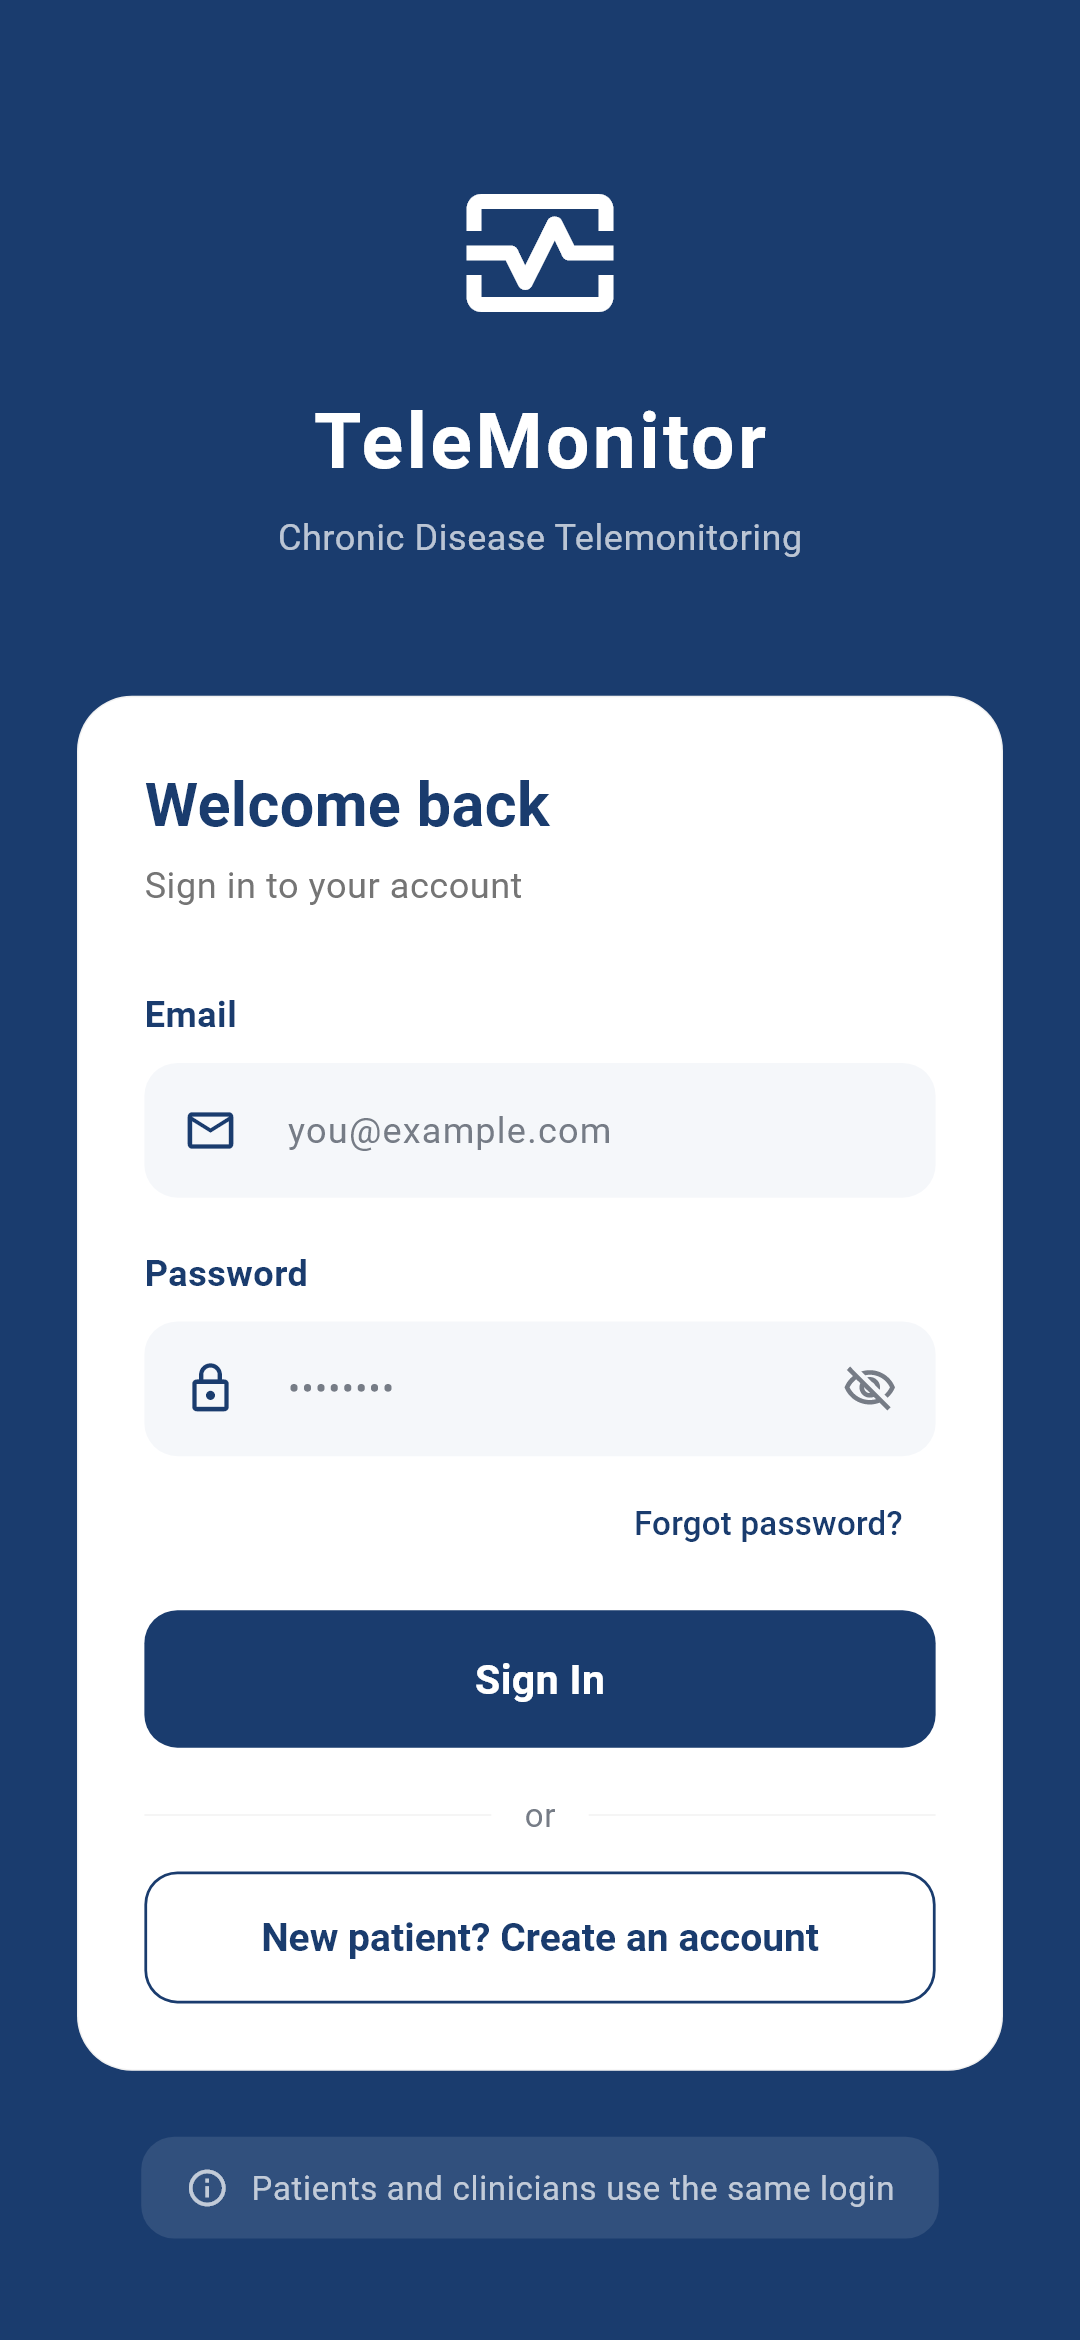
\includegraphics[width=\linewidth]{figures/screens/login_light.png}
  \caption{Sign-in}
\end{subfigure}\hfill
\begin{subfigure}[t]{0.17\textwidth}\centering
  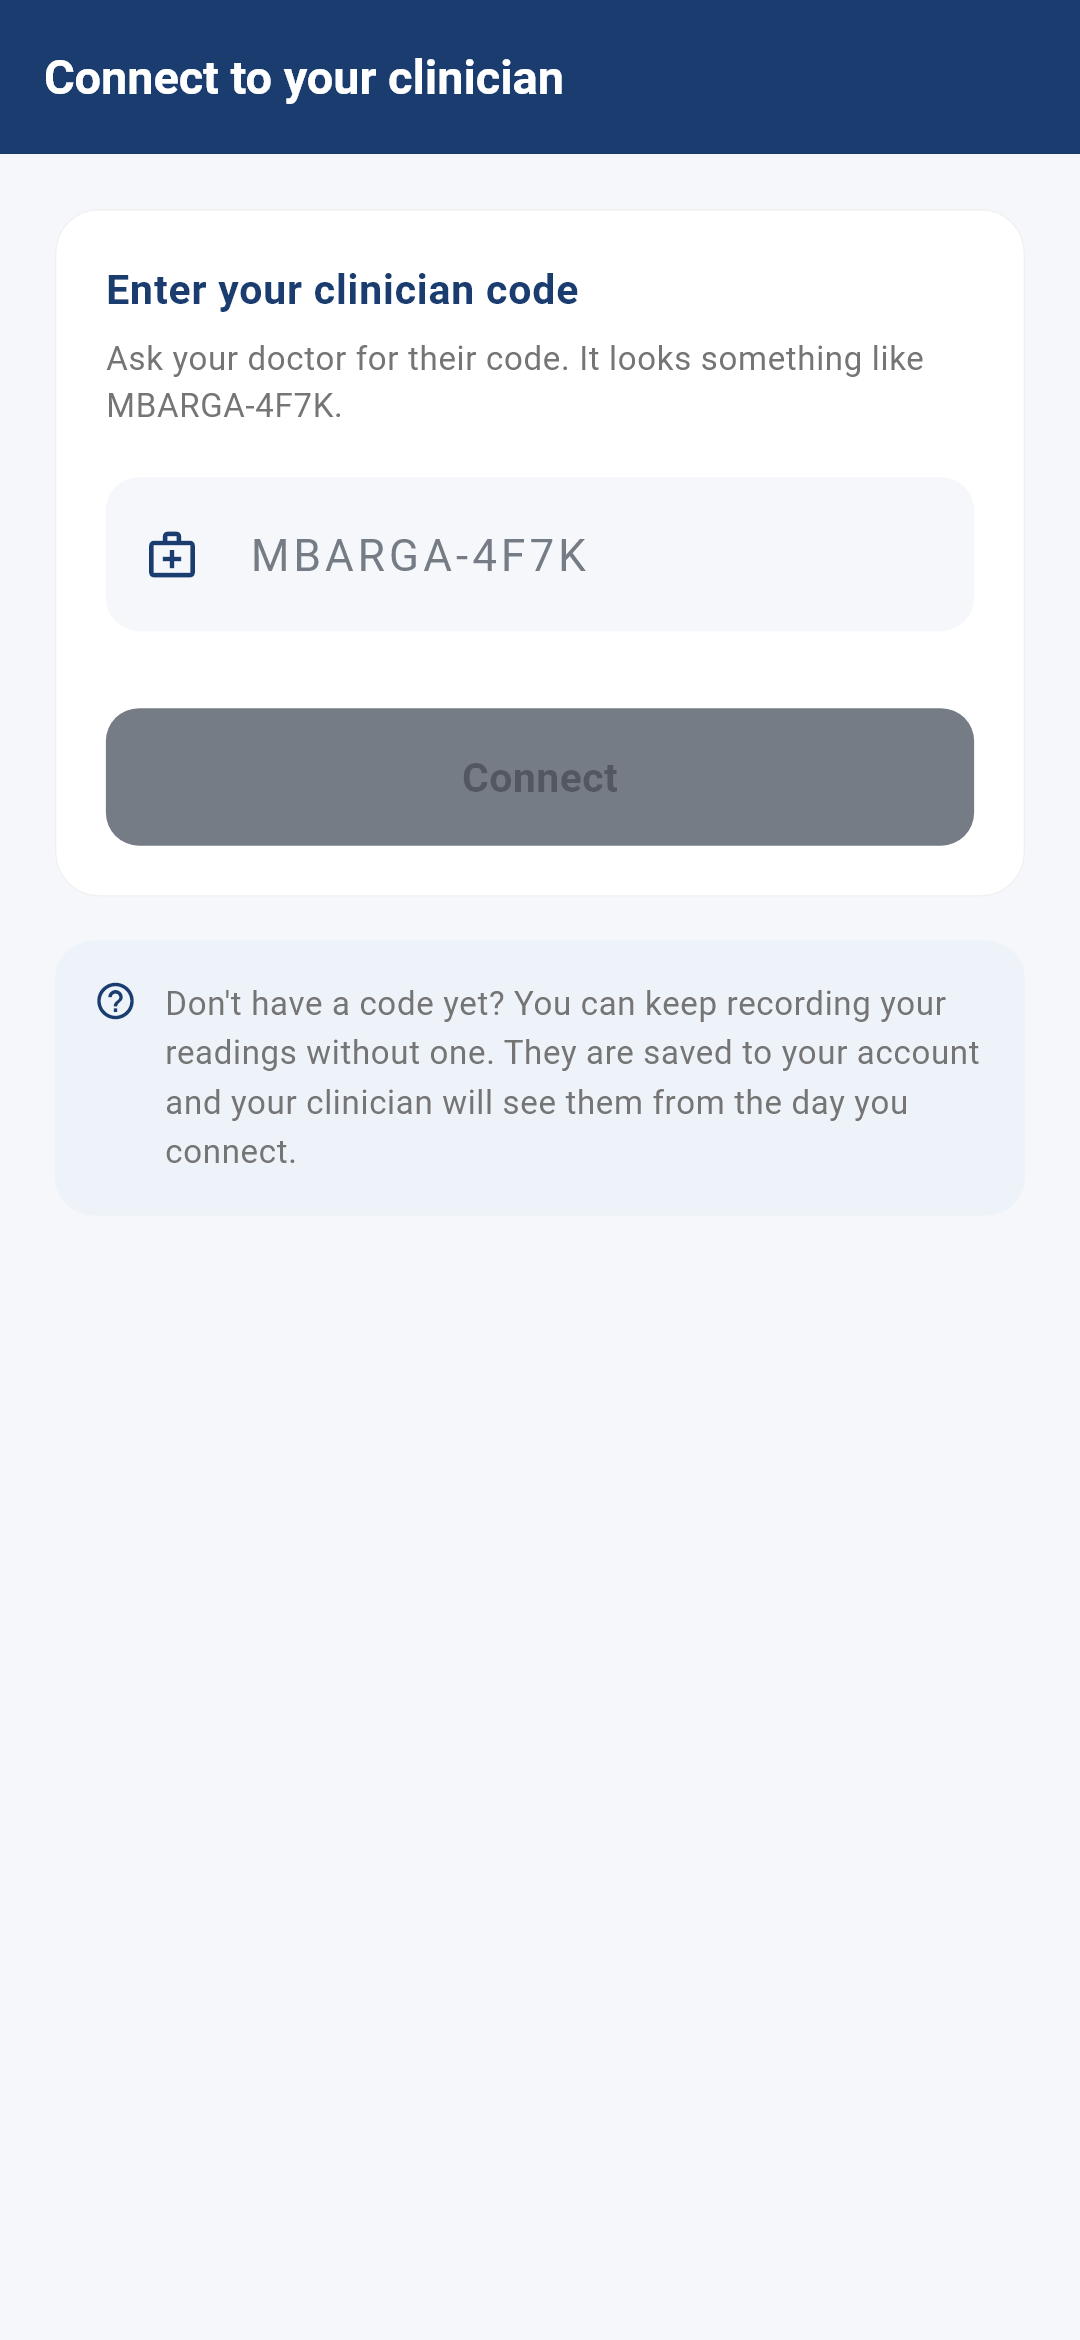
\includegraphics[width=\linewidth]{figures/screens/connect_clinician_light.png}
  \caption{Enrolment}
\end{subfigure}\hfill
\begin{subfigure}[t]{0.17\textwidth}\centering
  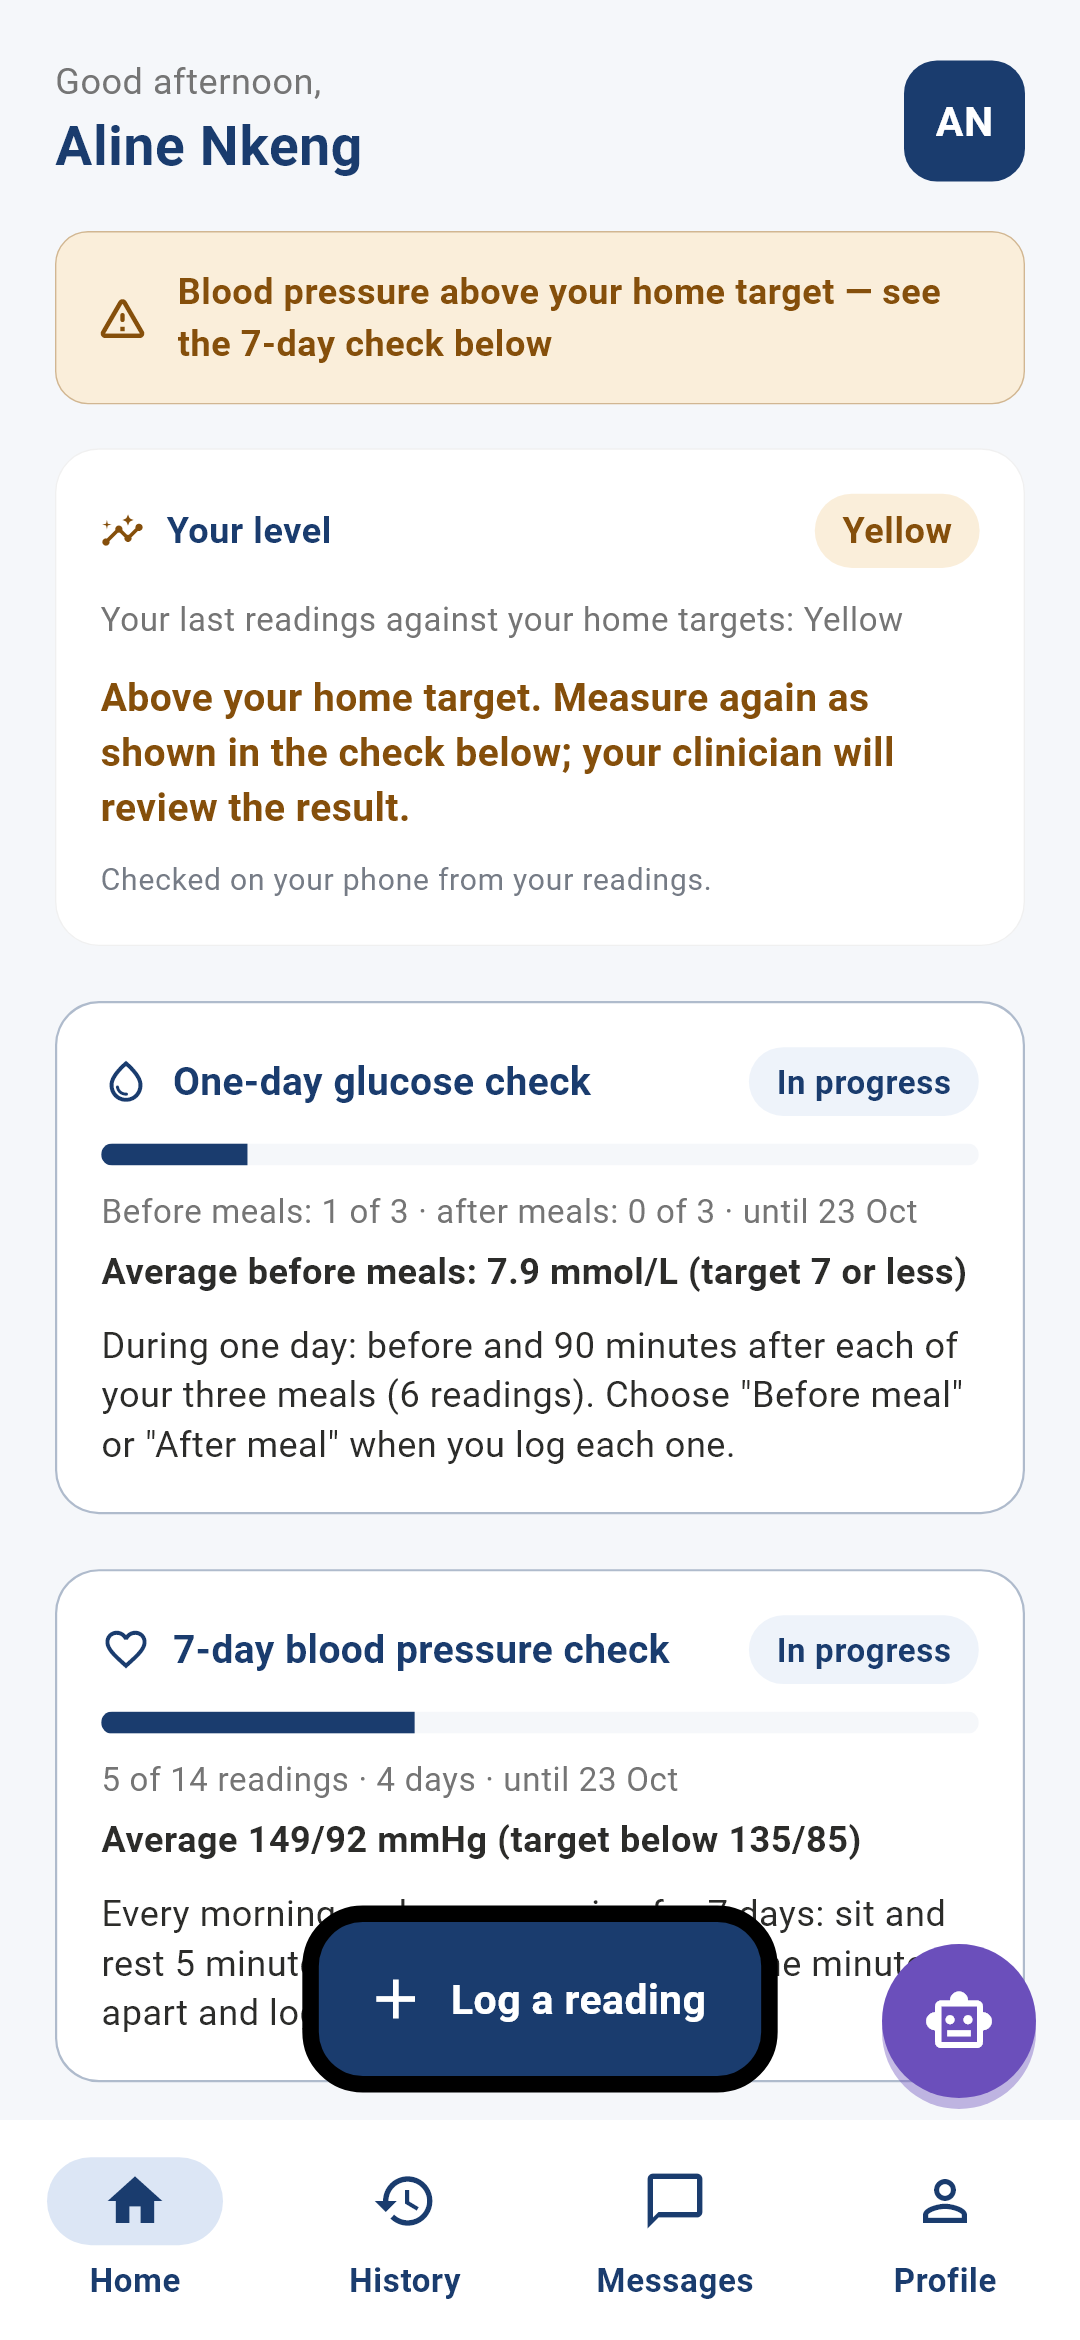
\includegraphics[width=\linewidth]{figures/screens/home_light.png}
  \caption{Patient home}
\end{subfigure}\hfill
\begin{subfigure}[t]{0.17\textwidth}\centering
  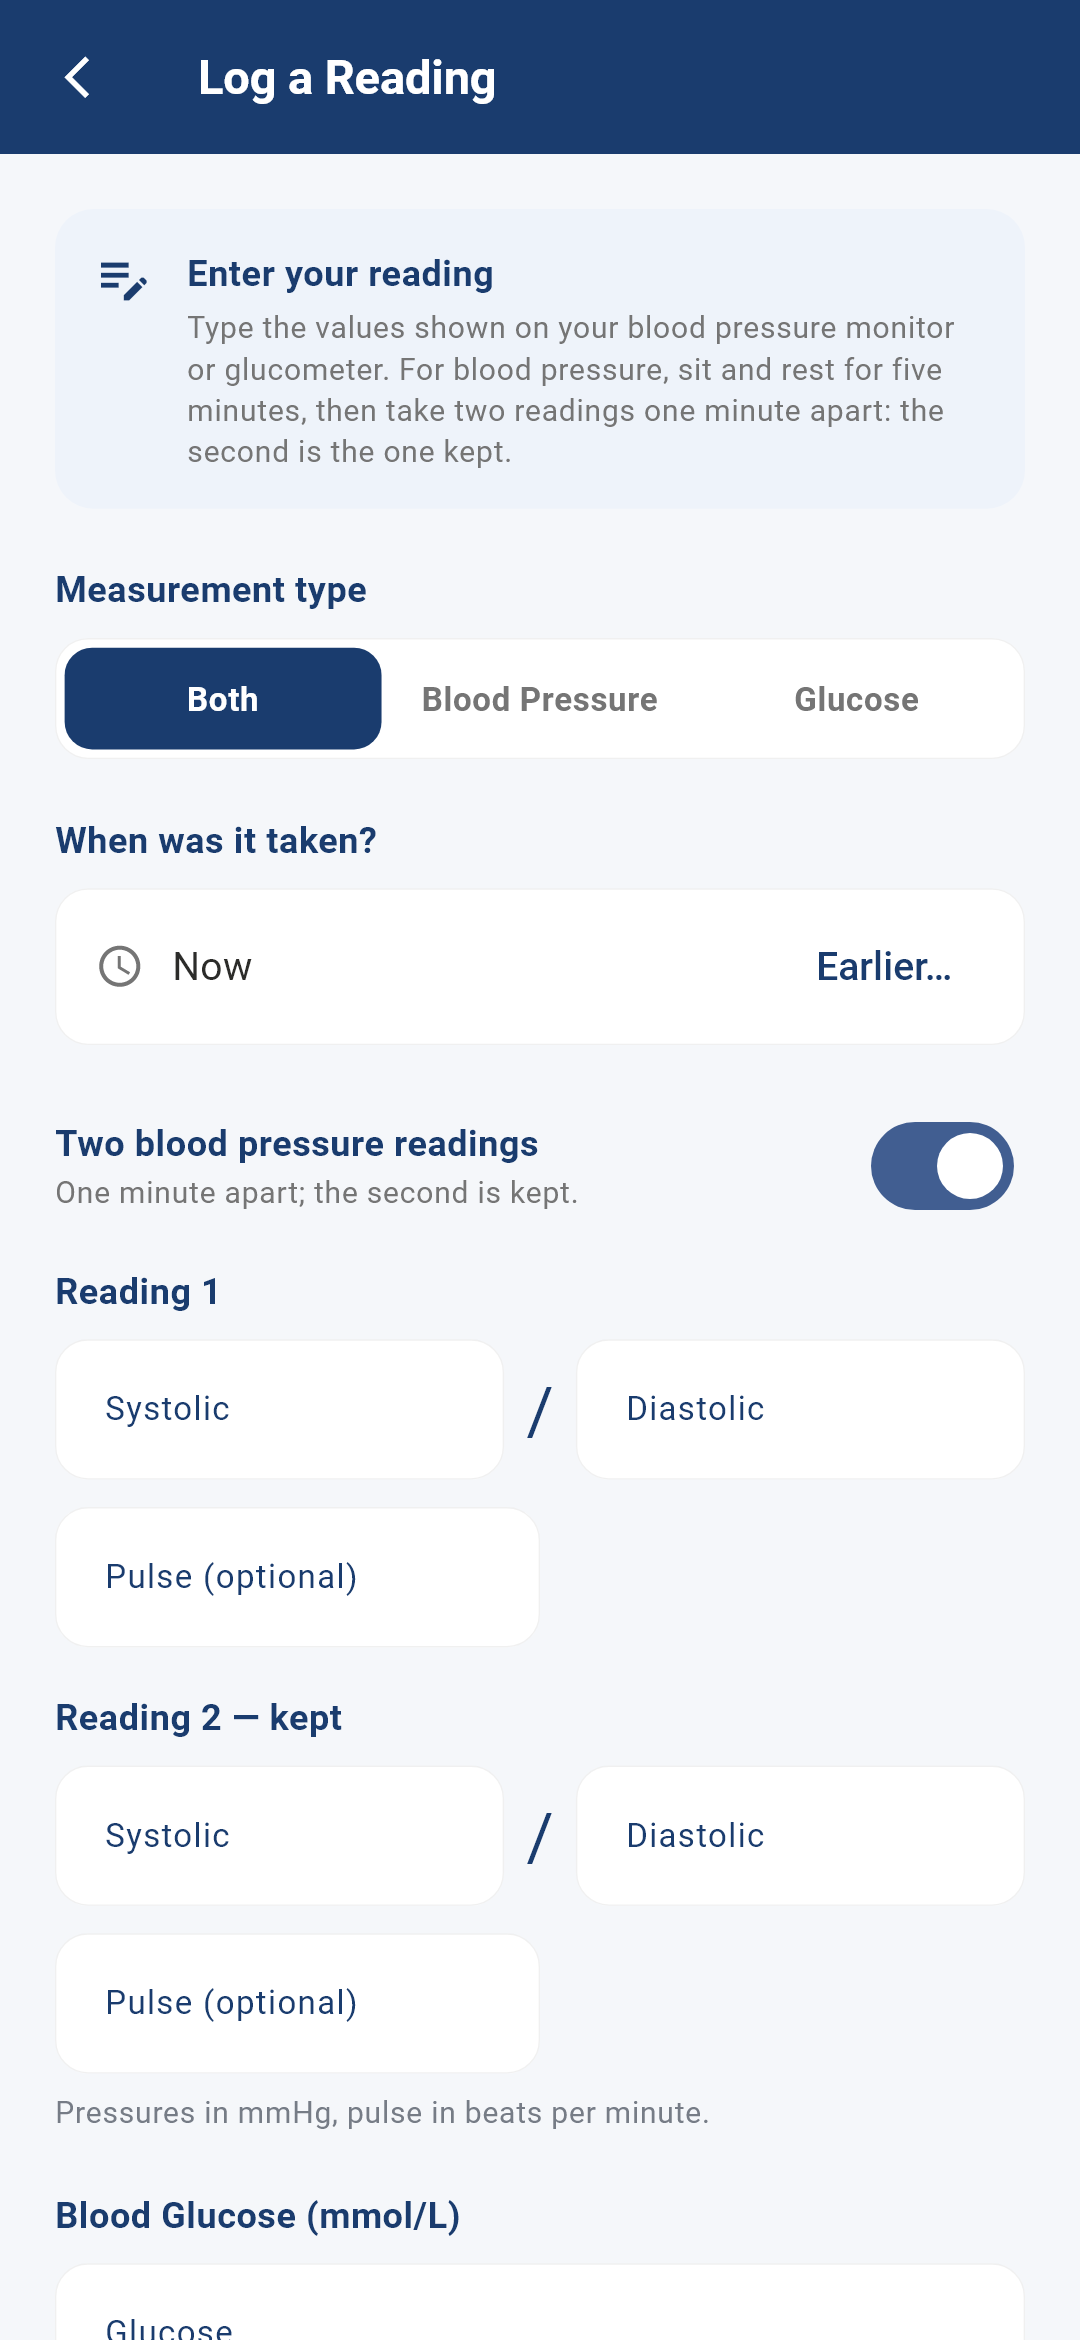
\includegraphics[width=\linewidth]{figures/screens/log_reading_light.png}
  \caption{New reading}
\end{subfigure}

\vspace{0.35cm}
\begin{subfigure}[t]{0.17\textwidth}\centering
  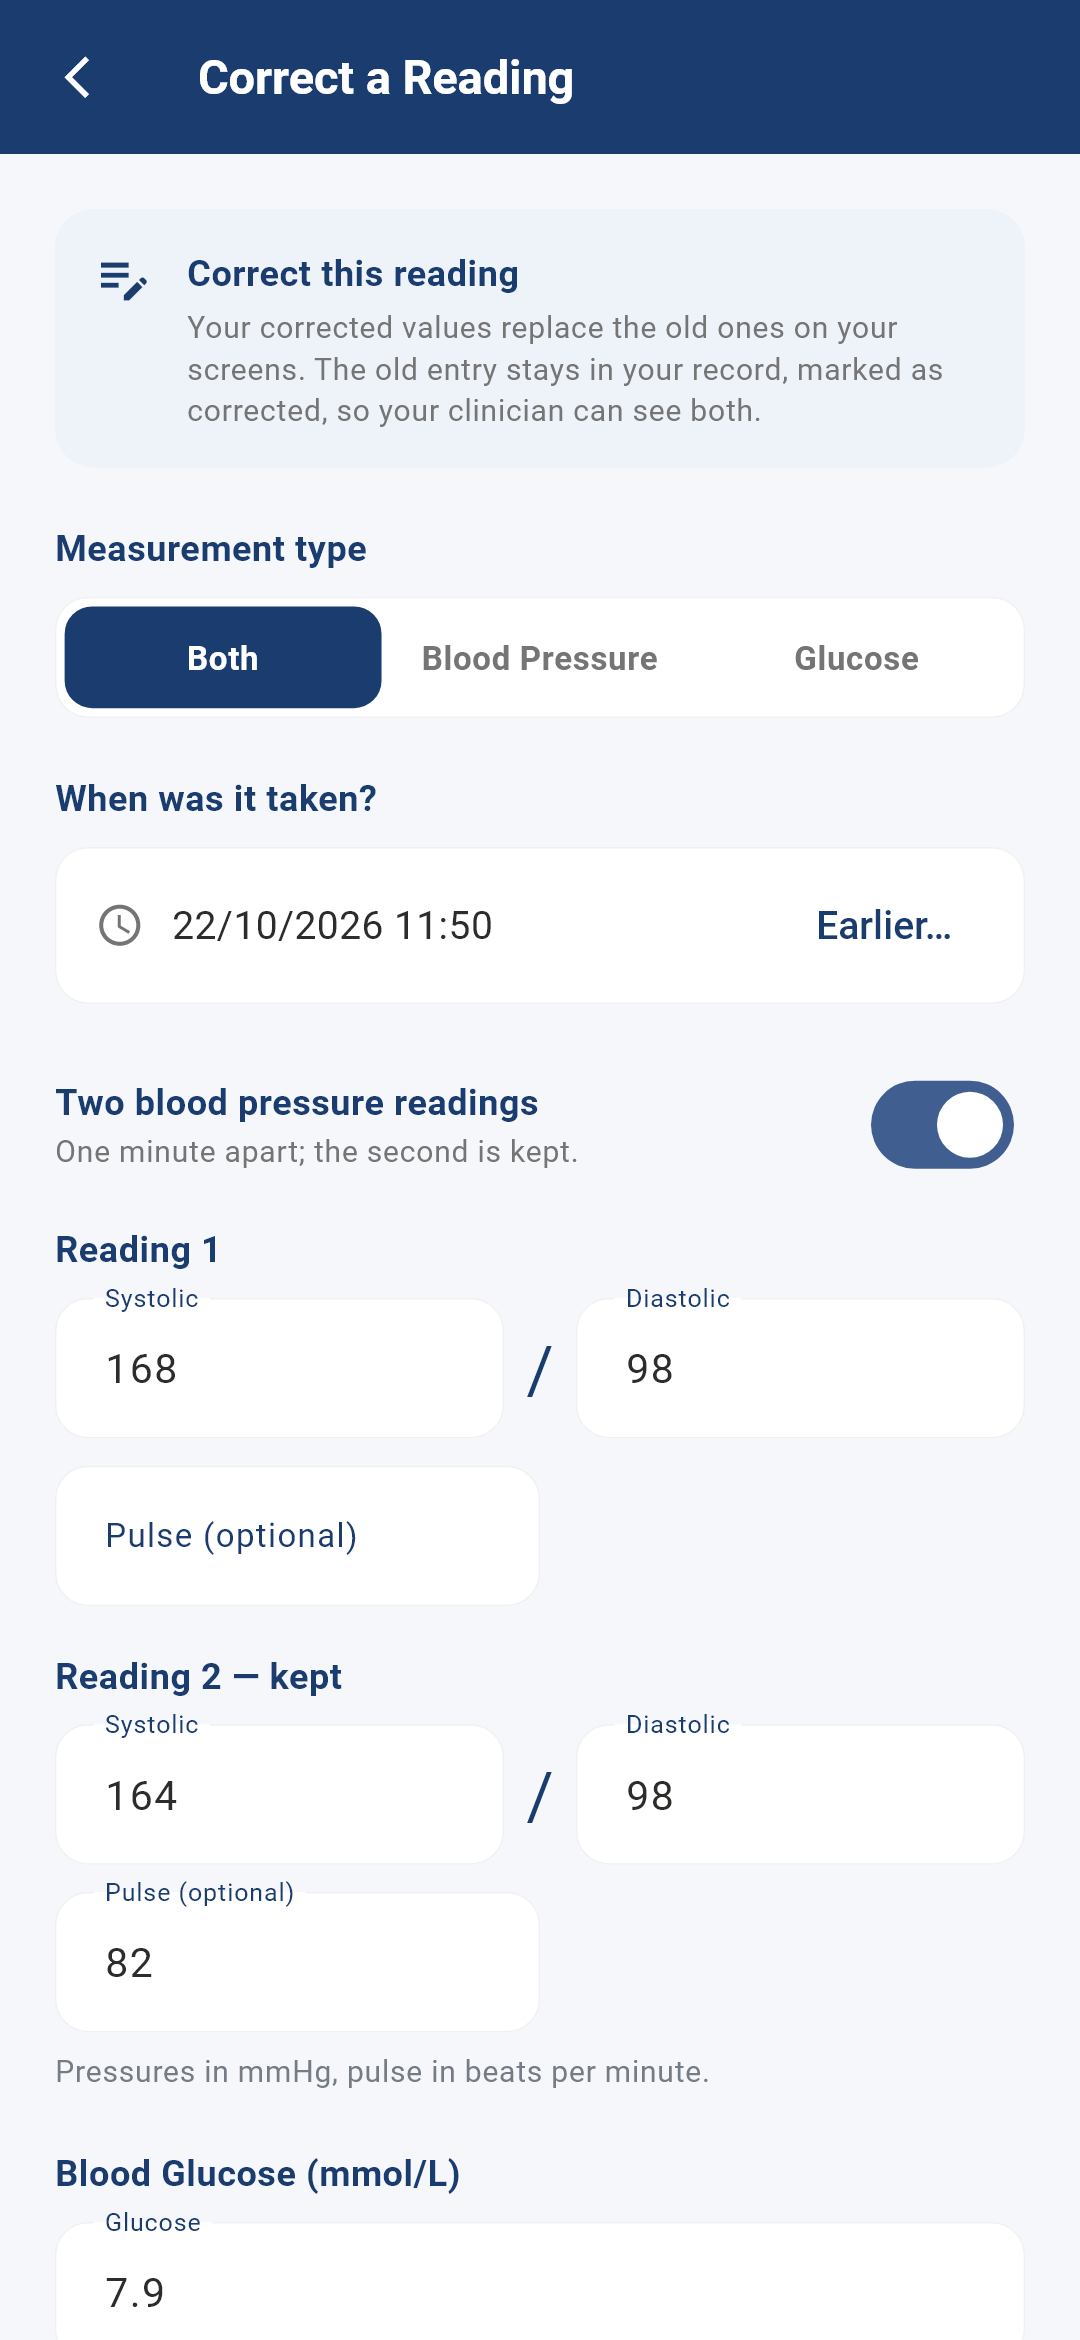
\includegraphics[width=\linewidth]{figures/screens/correct_reading_light.png}
  \caption{Correction}
\end{subfigure}\hfill
\begin{subfigure}[t]{0.17\textwidth}\centering
  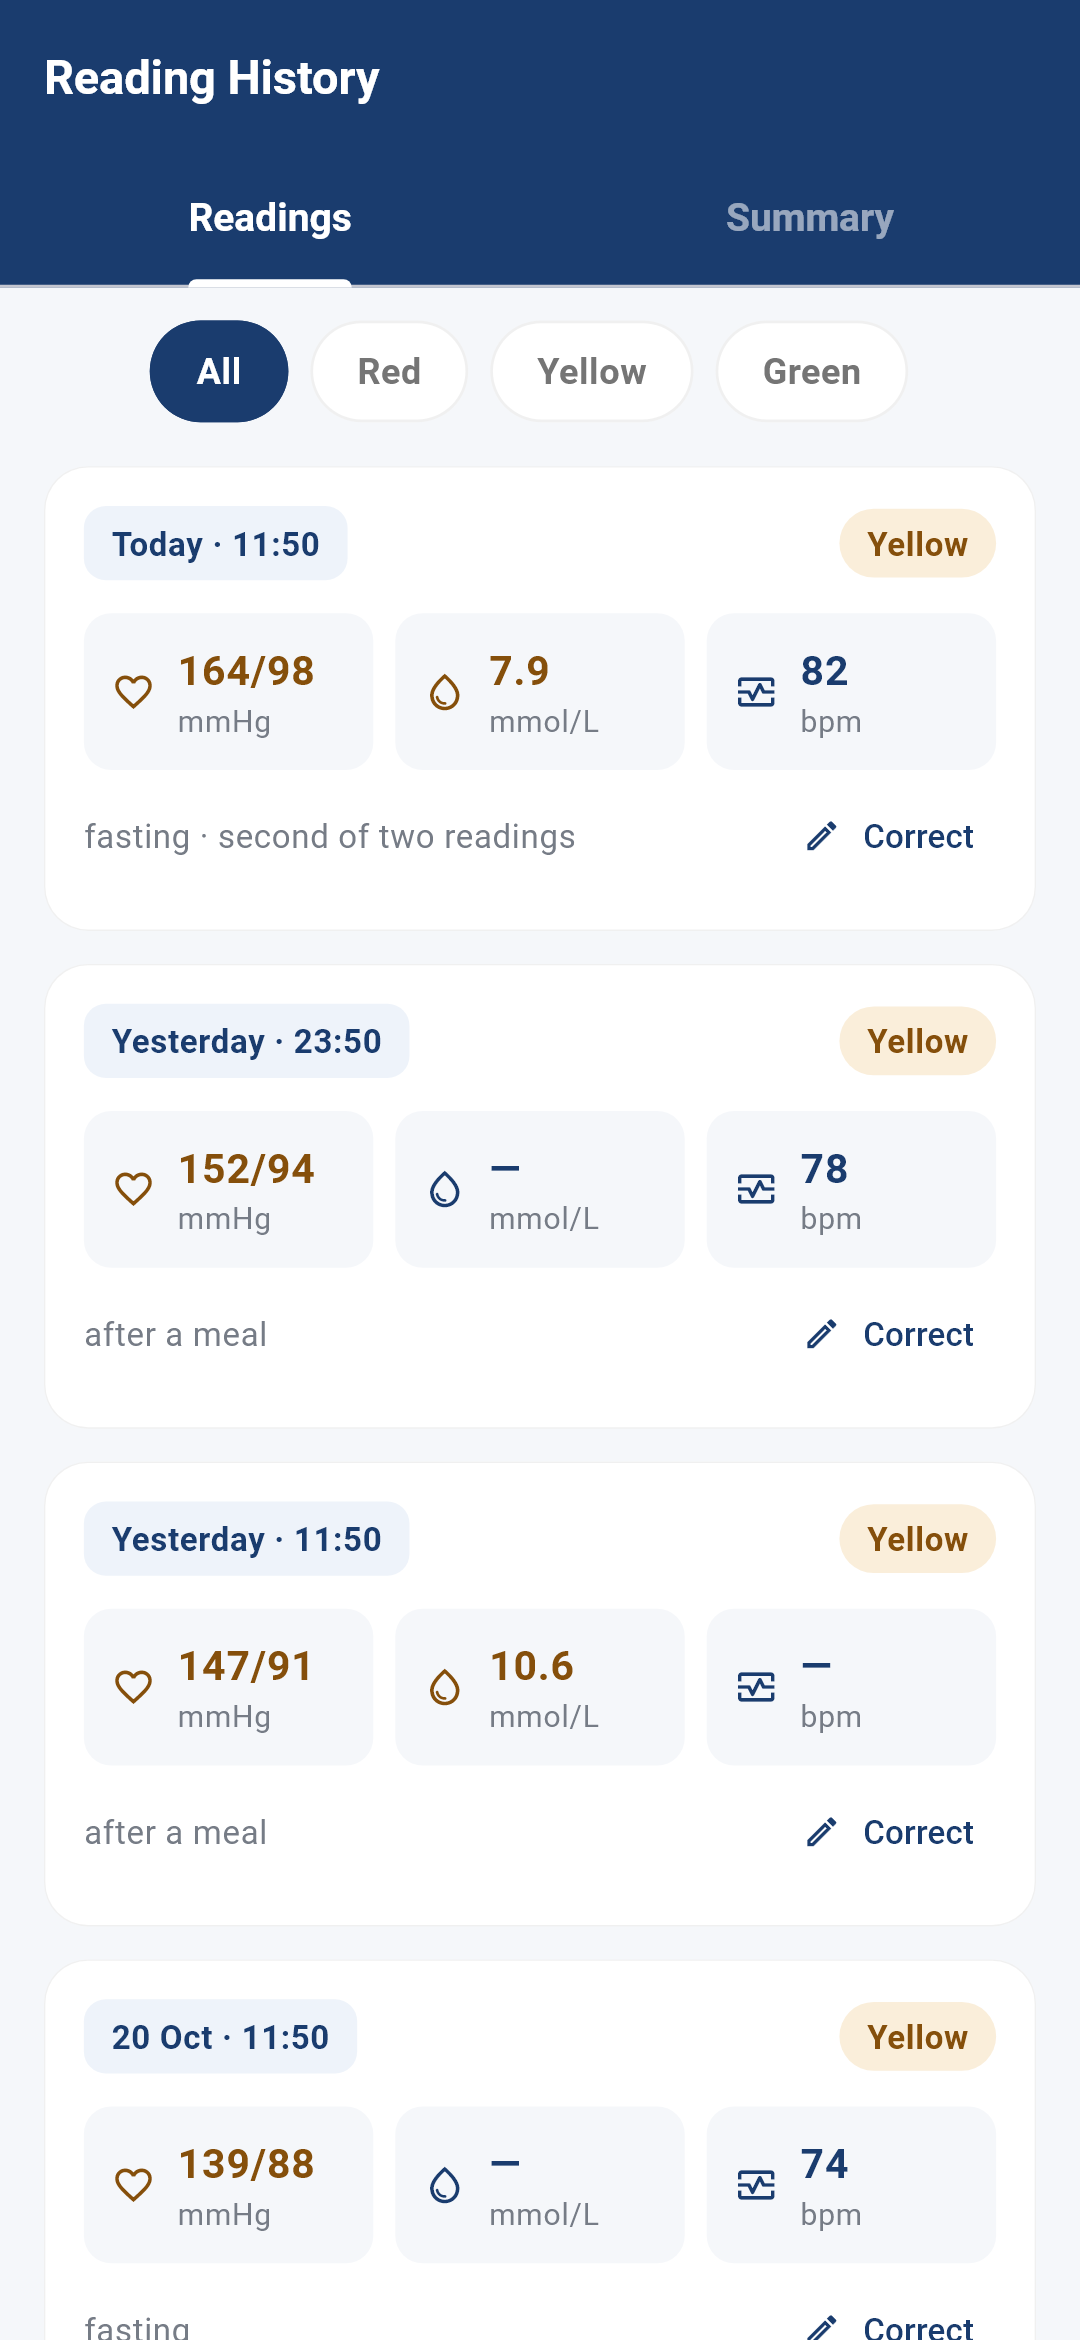
\includegraphics[width=\linewidth]{figures/screens/history_light.png}
  \caption{History}
\end{subfigure}\hfill
\begin{subfigure}[t]{0.17\textwidth}\centering
  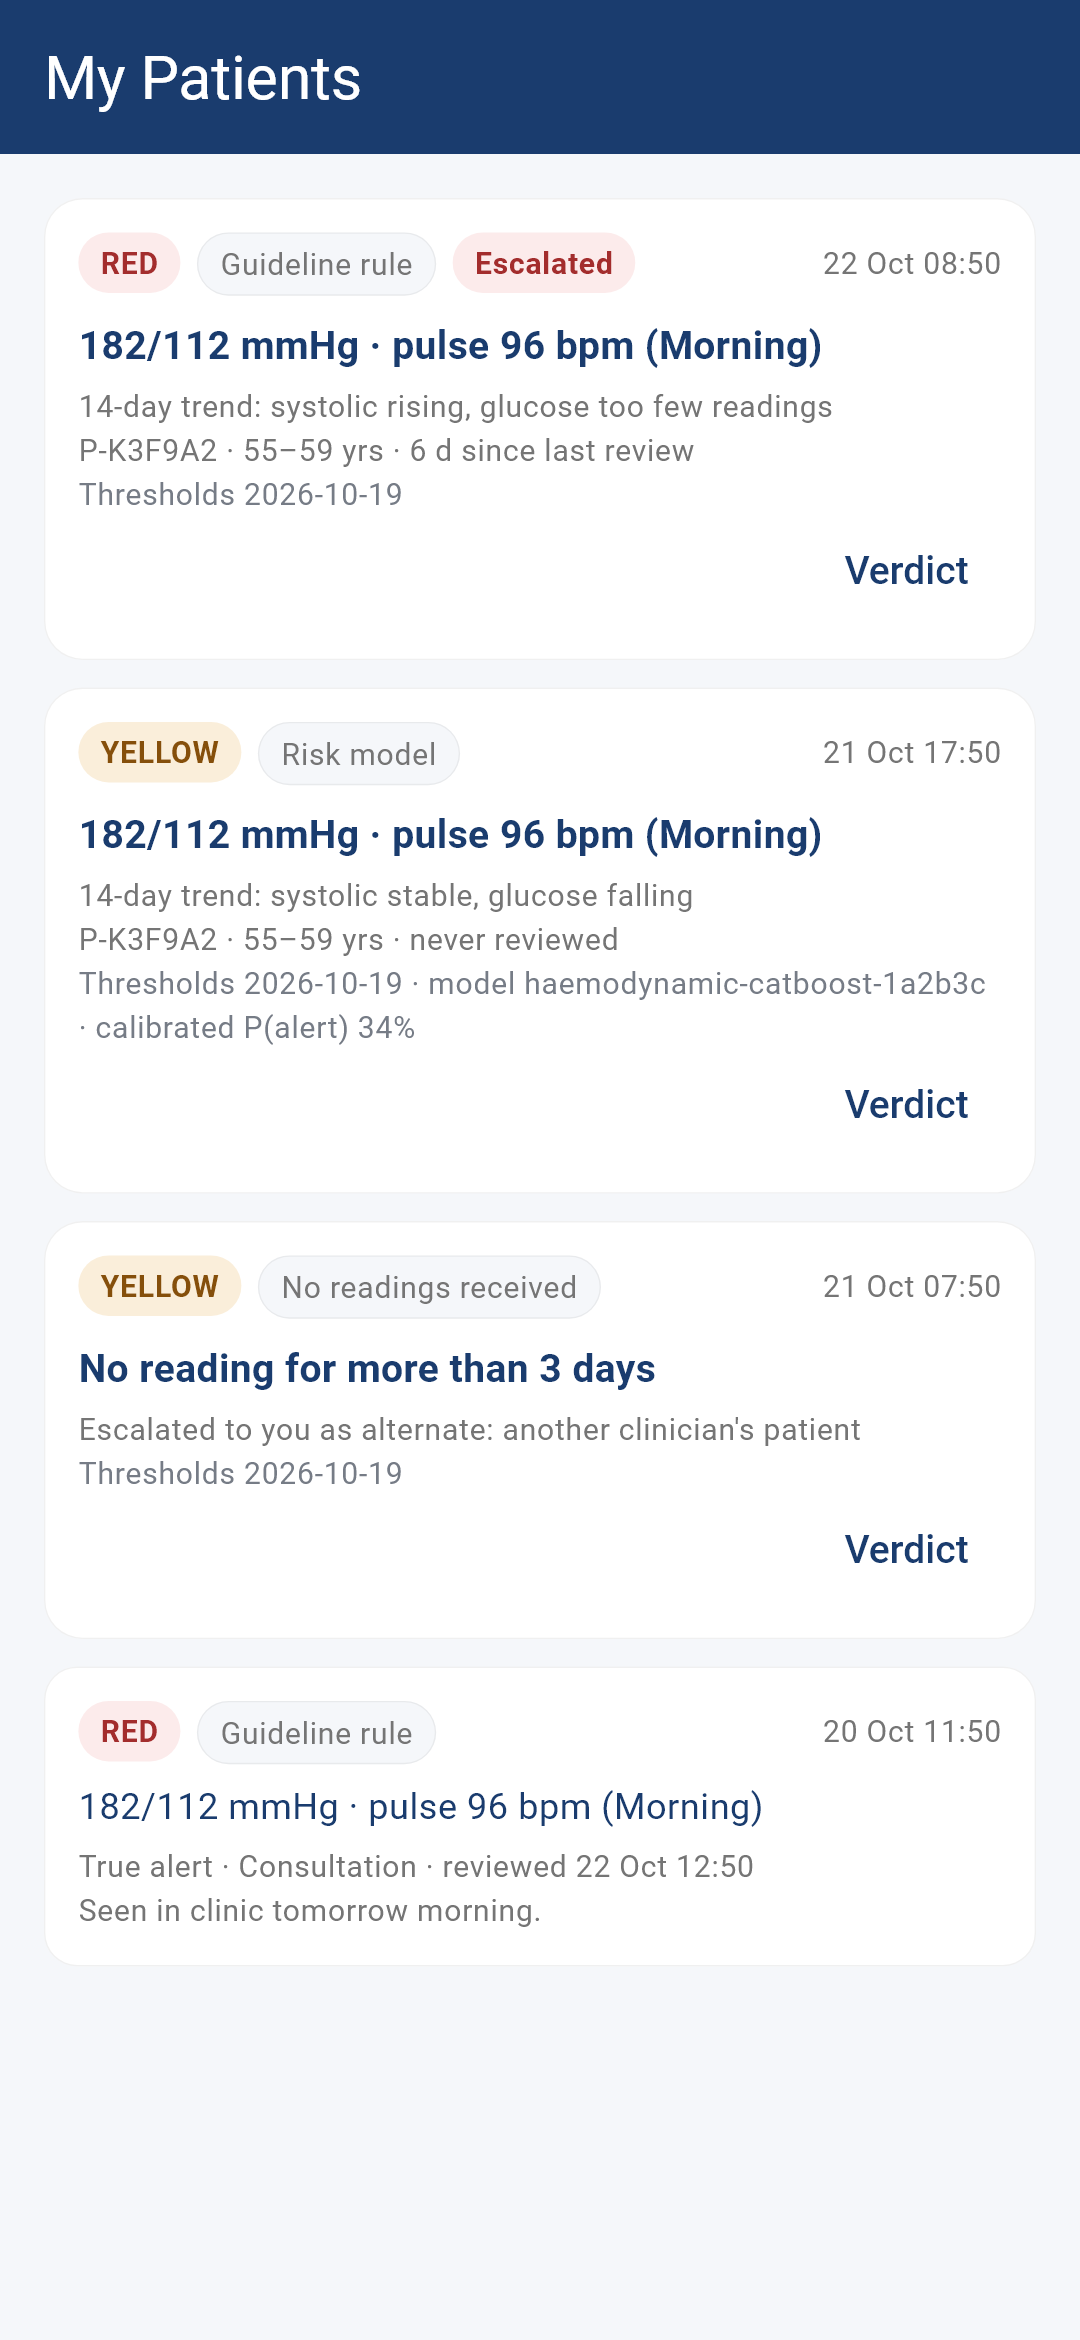
\includegraphics[width=\linewidth]{figures/screens/queue_light.png}
  \caption{Clinician queue}
\end{subfigure}\hfill
\begin{subfigure}[t]{0.17\textwidth}\centering
  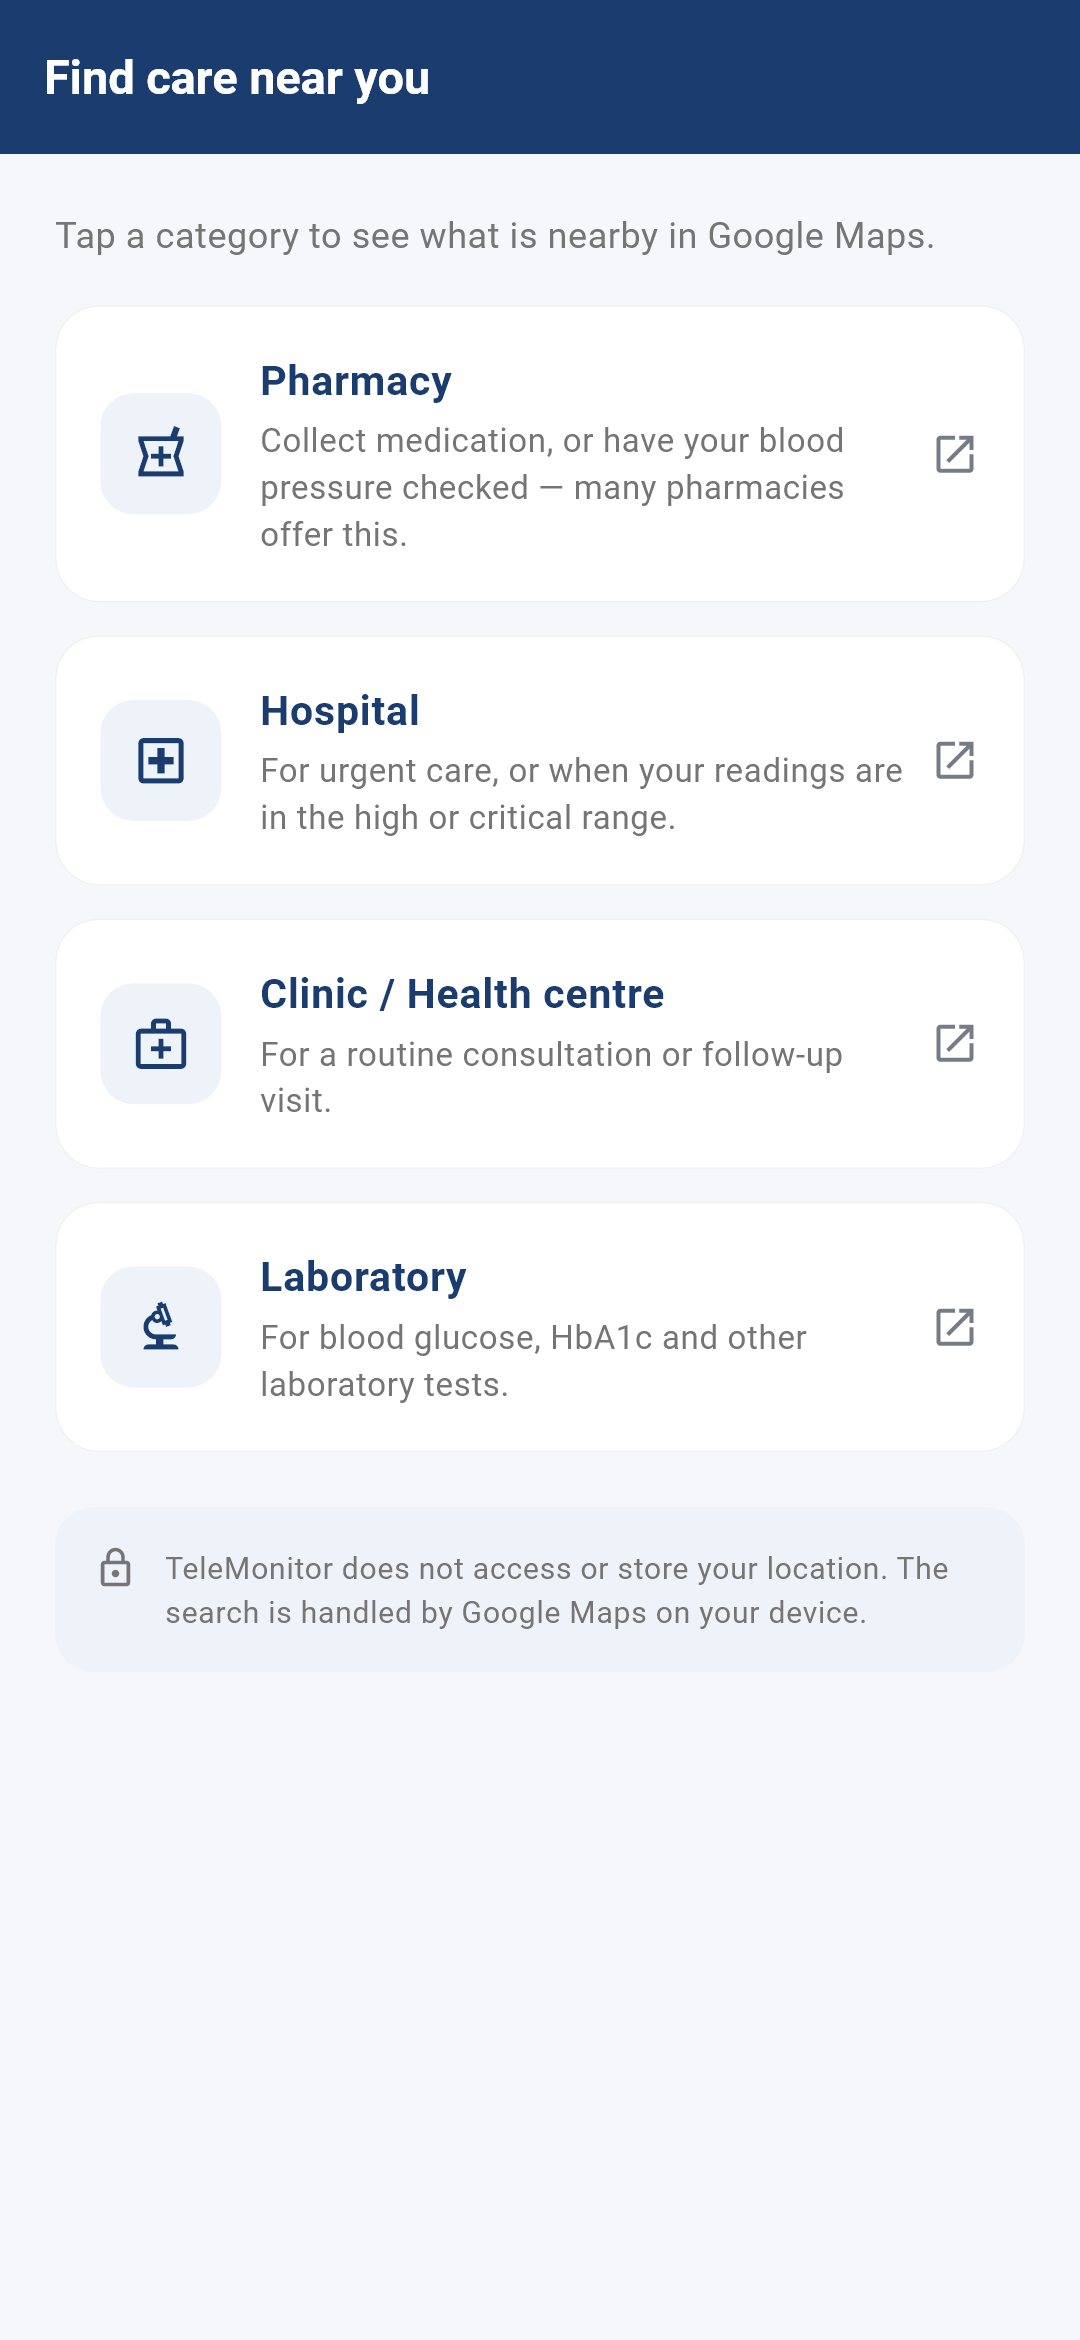
\includegraphics[width=\linewidth]{figures/screens/care_finder_light.png}
  \caption{Nearby care}
\end{subfigure}
\caption{Screens of the application: (a) sign-in, shared by patients and clinicians; (b) enrolment with the clinician's code; (c) patient home with the level, the instruction and the verification profiles; (d) entry of the two readings of the protocol; (e) correction, a new reading that supersedes the old one; (f) history with level and corrections; (g) clinician queue, red before yellow; (h) nearby care, opened in the phone's maps. Rendered by the widget tests with fictitious patients; model names and probabilities are test values.}\label{fig:screens}
\end{minipage}

\chapter{TRIPOD+AI Checklist}\label{app:tripod}

The modelling study is reported according to TRIPOD+AI \parencite{collins2024}; its risk of bias can be assessed with PROBAST+AI \parencite{moons2025}.

{\footnotesize
\begin{longtable}{@{}>{\raggedright\arraybackslash}p{1.1cm} >{\raggedright\arraybackslash}p{4.3cm} >{\raggedright\arraybackslash}p{8.6cm}@{}}
\caption{TRIPOD+AI items and where they are addressed.}\label{tab:tripod}\\
\toprule
\textbf{Item} & \textbf{Topic} & \textbf{Where} \\
\midrule
\endfirsthead
\toprule
\textbf{Item} & \textbf{Topic} & \textbf{Where} \\
\midrule
\endhead
1 & Title & title page \\
3a--c & Background, intended use, inequalities & Introduction; \cref{sec:lit-gaps} (Central Africa absent from the evidence) \\
4 & Objectives & Introduction (objectives, research questions, hypotheses) \\
5a--b & Data sources, dates & \cref{sec:data-collection}: Douala 2026; eICU 2014--2015; \cref{app:data} \\
6a--b & Setting, eligibility & \cref{sec:data-collection,sec:harmonisation}; \cref{app:data} \\
6c & Treatments & not recorded in either dataset \\
7 & Data preparation & \cref{sec:preprocessing} \\
8a--c & Outcome, assessment, blinding & \cref{sec:labelling}; blinded relabelling by the partner physician \\
9a--c & Predictors & \cref{sec:features}; instruments in \cref{sec:instruments-obtained} \\
10 & Sample size & \cref{sec:sampling,sec:results-sample-size} \\
11 & Missing data & \cref{sec:missingness} \\
12a--g & Partitioning, handling, model type, clusters, measures, updating, computation & \cref{sec:evaluation,sec:metrics,sec:ml,sec:tools}; outer folds by hospital; intercept update; \cref{app:config} \\
13 & Class imbalance & class weights and their correction (\cref{sec:evaluation}) \\
14 & Fairness & results by sex and age band (\cref{sec:metrics}) \\
15 & Output, thresholds & \cref{sec:tiers} \\
16 & Development against evaluation data & \cref{sec:results-data} \\
17 & Ethical approval & \cref{sec:ethics-considerations} \\
18c--f & Protocol, registration, sharing & protocol fixed before results; not registered; \cref{sec:tools} \\
19 & Patient and public involvement & none \\
20--27 & Results, discussion & \cref{ch:results} \\
\bottomrule
\end{longtable}
}


\end{document}
